\documentclass[a4paper]{article}

%% Language and font encodings
\usepackage[english]{babel}
\usepackage[utf8x]{inputenc}
\usepackage[T1]{fontenc}
\usepackage{acronym}
\usepackage{dcolumn}

%% Sets page size and margins
\usepackage[a4paper,top=3cm,bottom=2.5cm,left=3cm,right=3cm,marginparwidth=2.5cm]{geometry}

%% Useful packages
\usepackage{amsmath,amssymb}
\usepackage{graphicx}
\usepackage[colorinlistoftodos]{todonotes}
\usepackage[colorlinks=true, allcolors=blue]{hyperref}
\usepackage{xcolor}
\usepackage{listings}
\usepackage{color}
\usepackage{eurosym}
\usepackage{dirtree}
\usepackage{subcaption}


%% Colors
\definecolor{breeze}{RGB}{245,245,245}
\definecolor{mauve}{rgb}{0.58,0,0.82}

\definecolor{codegreen}{rgb}{0,0.6,0}
\definecolor{codegray}{rgb}{0.5,0.5,0.5}
\definecolor{codepurple}{rgb}{0.58,0,0.82}
\definecolor{backcolour}{rgb}{0.95,0.95,0.92}
 
\lstset{
    language=R,
    basicstyle=\small\ttfamily,
    stringstyle=\color{codegreen},
    otherkeywords={0,1,2,3,4,5,6,7,8,9},
    morekeywords={TRUE,FALSE},
    deletekeywords={data,frame,length,as,character},
    keywordstyle=\color{blue},
    commentstyle=\color{codegreen},
    backgroundcolor=\color{breeze},
    numbers=none
}
%%% Define Bibliography %%%
\usepackage{natbib}


\begin{document}

\makeatletter         
\def\@maketitle{
\begin{center}
{\huge \@title }\\[4ex] 
{\Large  \@author}\\[4ex] 
\@date\\[8ex]

\includegraphics[width = 40mm]{image_humboldt.png}
\end{center}}
\makeatother

\begin{titlepage}
\title{EMPLOYMENT EFFECTS \\ OF THE NEW \\ GERMAN MINIMUM WAGE \\ (SOEP DATA)}
\author{\textbf{Authors:} \\ Meret Borchmann, 573149 \\ Jupp Kerschek, 569920 \\ Albert Thieme, 565451 \\ Timm Walz, 576239 }

\date{March 2018}

\date{\parbox{\linewidth}{\centering%
  \today\endgraf\bigskip
  Humboldt-University of Berlin \endgraf
  School of Business and Economics \endgraf\bigskip
  \textbf{Subject:} \endgraf
  \bigskipamount =12pt
  Statistical Programming Languages\endgraf\bigskip
  Winter Term 2017/2018}}

\clearpage\maketitle
\thispagestyle{empty}
\end{titlepage}
\newpage 

\tableofcontents 
\setcounter{page}{1}

\newpage
 
\listoffigures
 
\listoftables

\section*{List of Abbreviations}
\begin{acronym}[Bash]
 \acro{CDU}{Christian-Democratic Union}
  \acro{CSU}{Christian-Social Union}
 \acro{CSV}{Comma Separated Values}
 \acro{CTA}{Common Trend Assumption}
 \acro{Dif-in-Dif}{Difference in Differences}
 \acro{DIW}{Deutsches Institut für Wirtschaft}
 \acro{DTA}{Stata Data File Format}
 \acro{PNG}{Portable Network Graphic}
 \acro{SOEP}{Sozioökonomisches Panel}
  \acro{SPD}{Social Democratic Party}
 \acro{STUVA}{stable treatment value assumption}
 \acro{URL}{Uniform Resource Locator}
 \acro{GADM}{Database of Global Administrative Areas}

\end{acronym}

\pagebreak
\section{Introduction}
\subsection{Motivation and Research question}
The \textit{great coalition} of Christian Democratic Union (CDU)/Christian-Social Union (CSU) and Social Democratic Party (SPD) introduced on the first January 2015 in Germany a region wide, statutory minimum wage of 8.50{\euro} per hour, after long term negotiations (\cite{bundestag}). The so achieved compromise is almost completely binding with only very few exceptions. Thus, the minimum wage introduction led to a German wide wage shock in regional labor markets. The introduction was accompanied by a huge debate questioning the effect on labor demand in particular.

This is because labor economic theory provides different employment outcomes depending on the labor market structure. In a neoclassic framework, the labor market is characterized by a competitive price market setting.  As a result, wage rises prior to the minimum wage introduction will lead to negative employment effects. Contrary assuming a monopsonic labor demand, the effect of the minimum wage is ambiguous and depends on the minimum wage level. It can be possible that labor demand rises if employees are paid below the marginal product of labor.
This leads to our motivation for this report, which is to identify the potential outcome of the introduction of the minimum wage in Germany on employment empirically. In order to identify the effect on employment, we use the \textit{Sozioökonomische Panel} (SOEP). According to the \textit{Deutsches Institut für Wirtschaft} (DIW), the SOEP is a wide-ranging representative longitudinal study of private households in Germany, thus it should be a suited dataset for us to use. 
Related to our motivation we developed the following research question for our report: „Employment effects of the new German minimum wage (SOEP dataset)“, hence we analyze the employment effect in a difference-in-difference (DiD) framework, similar to \cite{schmitz2017effects} and \cite{caliendo2017short}. 
\cite{schmitz2017effects} evaluates the introduction of the minimum wage in Germany on employment using country-level administration data in a DiD framework. In particular, using regional variation of the Kaitz Index as a measure to estimate the 'bite' in  the regional wage level due to the minimum wage introduction. In theory, if the bite in a certain region is stronger than in another, this region should be more affected by the minimum wage introduction. Consequently, if the employment effect differs across regions with different bites, this effect can be identified as the impact of the minimum wage introduction, ceteris paribus.
\cite{caliendo2017short} share the same identification strategy as \cite{schmitz2017effects}, however they use a different dataset. Specifically, they combine the SOEP and the Structure of Earnings Survey (SES) data and use the Kaitz as well as the Fraction Index for 141 regional labor markets in Germany. \\
We will analyze the regional effects on federal state level. While this means that we cannot estimate the effects in such great regional detail as in the mentioned research papers, it allows us to have a sufficient sample size. \\
The remainder of this report proceeds as follows. Section 2 introduces the data acquisition and preparation. In Section 3, the data is analyzed descriptively for a specific year, while Section 4 is about a simulation of the minimum wage effect with data prior to the minimum wage introduction. Subsequently, Section 5 displays descriptive results about the necessary employment variables and Section 6 identifies the affected regions. In Section 7, the analysis of the minimum wage effect is graphically visualized. Section 8 presents the main analysis of employment effects, while Section 9 displays several statistical tests to find out whether the model is correctly specified. Finally, Section 10 concludes.
Note that, given there is a corresponding statistical and econometric theory, these will be explained in each section accordingly.


\subsection{Repository Access}
The corresponding GitHub-repository for this project can be found following this uniform resource locator (URL):\\ \url{https://github.com/torsion214/spl-pirates}.\\
It contains the whole source code separated in eight quantlets, the associated SOEP input data, a README-file (for the project and for each quantlet) as well as this research report and the presentation conducted in January 2018. Each quantlet has an own directory, which is named based on the following notation: \\ \textit{SOEPQ[number of quantlet, 1-8]\_[Name of Quantlet]}\\  The source code was built to be executable at any system running RStudio with the packages documented in chapter \ref{rpackages}.

\subsection{Preparation of the Working Directory} 
Basically, it does not matter where the working directory is stored on the system, as the source code uses relative paths. It is just important to set the working directory, where the \textit{InstallPackages.R}-file is located, which is the home directory of the repository \textit{spl-pirates}.  
This is really important to execute the quantlets correctly, as the execution is always initiated by the root directory. \\ 
\textbf{Examples: }\\
Right => setwd(\textit{"/Your/Local/Structure/spl-pirates"}) \\  
Wrong => setwd(\textit{"/Your/Local/Structure/spl-pirates/SOEPQ1\_ImportPrepareData"}) \\

The quantlets are ordered by numbers (Q1-Q8) and it is strongly recommend to execute them number-by-number, as the quantlets partly refer to previously created objects and variables. In the \textit{metadata.txt} as well as in the \textit{README.md} of each quantlet, the exact quantlet-dependencies are listed. Q1 and Q6 require input data. For Q1, they need to be stored in a subfolder \textit{input-data}, which contains further subfolders for each year. They have to be named with respective year.
This notation has to be kept strictly, as the name of directory identifies the year of the data stored in the underlying folder. If it is considered to add further waves (e.g. the dataset for 2017 being published next year), another directory has to be created in the \textit{input-data} directory with the respective year (then called 2017). The desired input data has to be stored inside this folder.
Within the \textit{variable-selection}-folder in Q1, the \textit{comma-separated values} (csv)-file with the labels and variable selection is located. The plots and graphs created with the source code will be saved in the \textit{plots}-folder of each quantlet, if the source code generates any. This is the case for Q2-Q6. Each quantlet folder also contains each generated plot as \textit{Portable Document File} (pdf). Within the quantlet folder of Q6, there is also a subdirectory \textit{geodata} containing the data for the map of Germany.
The directory tree is illustrated in figure \ref{figure:tree}.

\begin{figure}
  	\caption{Directory tree of the project} 
  	\label{figure:tree} 
\dirtree{%
.1 spl-pirates.
.2 SOEPQ1\_ImportPrepareData.
.3 input-data.
.4 2010, 2011, 2012, 2013, 2014, 2015, 2016.
.3 variable-selection.
.2 SOEPQ2\_DescriptiveAnalysis.
.3 plots.
.2 SOEPQ3\_SimulationMinimumWageEffect.
.3 plots.
.2 SOEPQ4\_EmploymentAnalysis.
.3 plots.
.2 SOEPQ5\_IdentificationAffectedRegions.
.3 plots.
.2 SOEPQ6\_GraphicalAnalysisMinWage.
.3 geodata.
.3 plots.
.2 SOEPQ7\_DiffDiffEstimation.
.2 SOEPQ8\_StatisticalTests.
}
\end{figure}


%%%%%%%%
%%Next Section%%
%%%%%%%

\section{Data Acquisition and Preparation}
\subsection{Introduction}
Basically, the SOEP datasets are free of charge. Nevertheless, a registration at the SOEP platform had to be completed for the data acquisition. The access to the platform was successfully granted. As the data is stored in a protected area and requires a license key, the data cannot be downloaded directly into the repository using a download script in R. Hence, they have to be downloaded and manually put into the destination folder.

The data can be ordered at the website of SOEP following this URL:\\
\url{https://www.diw.de/de/diw_01.c.345693.de/soep_bestellformular.html}\\
The data is available for the years 1984 - 2016. For the single years, they are called \textit{waves} (original German translation: \textit{Wellen}). This analysis covers the waves of 2010 - 2016 (identifiers a - g). The most recent dataset is called v33 (Wave BG) and includes the entire data over the years.

Back then, the presentation of this research topic only dealt with the datasets from 2010 - 2015, as the survey data of 2016 was not published yet. At this point, the dataset of 2015 was the first and only one tracking the impact of the minimum wage amendment, as this law has been introduced beginning of 2015. As the data for 2016 could finally be acquired in February 2018, it has been added to the research focus. Therefore, it is part of the analysis in this paper as well. This enables more in-depth and representative insights into the effects of the minimum wage introduction in Germany as well as the opportunity to compare two distinct years. The SOEP provides multiple \textit{pdf}'s as a dataset description. Here, the subsets as well as the respective variables are described more in detail.

\subsection{Theory}
The survey data collected by SOEP is split into multiple subsets, as the subsets are specialized for certain topics. Again, these subsets contain multiple variables. The variables have a cryptic identifier, which makes it difficult to deal with the data without having additional information. Over the years, the meaning of the variables may be the same, yet the identifiers differ. Therefore, it is not recommendable to deal with the data in R without having a proper label, as it would be hardly reproducible. Each survey participant has a unique identifier \textit{persnr}, which is available in every year and the same throughout. However, the group of participants differs over the years. The data of a participant occur in multiple chunks.  \newline \newline
The subsets are provided as \textit{Stata Data File Format} (.dta) each. This format is the default data type of the software \textit{Stata}, a concurring product of R within the market for statistical software. The advantage of this format compared to conventional files like \textit{.csv} are the embedded labels, which makes it more comprehensive to deal with the data (e.g. variable identifier in 2016: \textit{bgp99h01}, label: \textit{Unemployment Benefit}). Nevertheless, they are not available and importable in R, as the software cannot deal with this kind of additional meta information from \textit{Stata}. Therefore, they have to be acquired by either importing them into \textit{Stata} or from the website of SOEP by searching for the variable identifiers. Within this project, the first one of the mentioned approaches has been applied.

The second letter, exemplary marked as "[\textit{x}]" above, is the identifier for the certain year. Every year, this value is substituted by an ascending letter. The rest is similar over the years. 
As an example, the identifier of the year 2015 is \textit{f}, so the codes for the respective datasets are \textit{bfp, bfpgen and bfpkal}.
As described before, the data is split in multiple subsets. However, it is sensible for an analysis to merge the data for enabling a wide-ranging overview.

Following data chunks from the SOEP waves mentioned above (2010 - 2016)  were selected for the analysis:
\begin{itemize}
\item{b[\textit{x}]p}
\item{b[\textit{x}]pgen}
\item{b[\textit{x}]pkal}
\item{b[\textit{x}]pequiv}
\end{itemize}

Based on the research question and the insights the research team wanted to gain, the variables were selected from the dataset. \newline
Altogether, the SOEP dataset comprises several gigabytes. Therefore, it would be too resource-consuming to proceed the whole data in one repository. For gaining insights about the predefined goal of this paper, only a subset of the entire SOEP data collection is required. Therefore, it is sensible to select the necessary variables beforehand, extract these from the whole dataset and only keep this selection in the analysis process. 
It turned out that the data selection process is time consuming and requires accuracy. The questionnaires vary over the years as the intended purposes are different and they get aligned depending on the current socio-economic demand. Partly, the variable names differ over the years, wherefore they have to be selected separately. To enable a comprehensible variable selection process, a .csv-file was created as a tracking sheet. This .csv-file contains the label of the variables in the first column, which are the same over the years, and a column for each year which is included in the analysis. This file is easily extendible with tools like Microsoft Excel or any Open Source Software for spreadsheets to include further years in the analysis. Using Excel etc. for editing the file is just a recommendation, as .csv-files can be opened with any conventional text-editor, which are included in operating systems by default. \newline 
One of the most important quality criteria for the source code was to offer the possibility of being able to proceed the SOEP datasets from any years with the software. Therefore, it was crucial to create a dynamic program code. The code does not have to be changed in case another year. It is only needed to add a column for the certain year and the related variable identifiers, which match to the label in the certain row. Those variables which do not occur in a certain year and therefore do not match to a label mentioned in the first column are marked as missing values \textit{"NA"} (abbreviation for \textit{not available}).

The following table \ref{table:variablelist} deals as an overview for the selected years, datasets and the amount of variables for the analysis.

\begin{table}[htbp]
\centering
\caption{List of used waves and number of variables} 
\label{table:variablelist} 
\begin{tabular}{|r|l|l|r|}
\hline
\multicolumn{1}{|l|}{\textbf{Year}} & \textbf{Identifier} & \textbf{Selected Datasets} & \multicolumn{1}{l|}{\textbf{Amount Selected Variables}} \\ \hline
\textbf{2010} & a & bap, bapgen, bapkal, bapequiv & 90 \\ \hline
\textbf{2011} & b & bbp, bbpgen, bbpkal, bbpequiv & 82 \\ \hline
\textbf{2012} & c & bcp, bcpgen, bcpkal, bcpequiv & 86 \\ \hline
\textbf{2013} & d & bdp, bdpgen, bdpkal, bdpequiv & 82 \\ \hline
\textbf{2014} & e & bep, bepgen, bepkal, bepequiv & 90 \\ \hline
\textbf{2015} & f & bfp, bfpgen, bfpkal, bfpequiv & 111 \\ \hline
\textbf{2016} & g & bgp, bgpgen, bgpkal, bgpequiv & 101 \\ \hline
\end{tabular}
\label{}
\end{table}

The selected data chunks mentioned in column \textit{Selected Datasets} above are stored in the respective Github-repository of this paper.
The dataset of 2015 and 2016 tend to contain more variables than the years before as the minimum wage has been introduced in Germany. These additional variables describe the impacts of this new amendment for the most part.

\subsection{Implementation in R}
\subsubsection{Used R-Packages}
\label{rpackages}
For solving the research problem, further R-packages were used beside the basic equipment of the framework. All of them are available for free and can be downloaded with the packet manager using \textbf{install.packages(‘[name of the package]‘)}-command. To make sure every package is installed before executing the source code, it is recommended to execute the \textbf{InstallPackages.R}-file, which is located in the home directory of the repository. The code creates a list of all necessary packages and performs the installation via \textbf{lapply}.

\begin{lstlisting}[firstnumber=1]
# Vector with names of all packages
list_packages = c("foreign", "stringr", "data.table", "stargazer", "dplyr", 
	"sp", "plm", "lmtest")
# lapply on the package vector
lapply(list_packages, install.packages)
# Delete the package vector again
rm(list_packages)
\end{lstlisting}

In table \ref{table:packagelist}, the included packages are listed and briefly described.

\begin{table}[htbp]
	\centering
  	\caption{Additional packages used within quantlets} 
  	\label{table:packagelist} 
    \begin{tabular}{|c|p{10cm}|p{1,5cm}|}
    \hline
    \textbf{Package name} & \textbf{Functionality} & \textbf{Used in} \\ \hline
    \textbf{data.table}   & Merge and manipulate large datasets, requires less time and computing power than standard packages             & Q1                 \\ \hline
    \textbf{dplyr}        & Alternative package for data manipulation, clearly arranged filtering of program code and easy generation of new columns        & Q2, Q3, Q4, Q5, Q6, Q8                 \\ \hline
    \textbf{foreign}      & Tool for importing foreign file types such as \textit{.dta} (Stata data)             & Q1                 \\ 
    \hline \textbf{ggplot2} & Plot system for R with a wide range of functions and a high degree of detail & Q2, Q3, Q4, Q5, Q6  \\
\hline \textbf{plm} & Functions for estimating models and conducting robust checks & Q7  \\
\hline
    \textbf{lmtest}           & Test functions for diagnostic checking in linear regression models              & Q8                 \\ 
    \hline
    \textbf{sp}           & Package for processing spatial data such as geographical maps             & Q6                 \\ 
    \hline \textbf{stargazer} & Generation of \LaTeX{} code from the R output, such as regression tables & Q2, Q7  \\
    \hline
    \textbf{stringr}      & Tool for manipulating text strings, required for extracting the year numbers             & Q1, Q2                 \\ \hline
    \end{tabular}
\end{table}



Every R-script within this research has the \textbf{library([name of the package])} function with the respective package on top, to make sure that it is loaded within the current session.
The foreign package enables the import of Stata-data, as it cannot be imported to R with the default import functions.

\newpage

\subsubsection{Implementation of the Data Preprocessing and Import (Q1)}
Since data import and data preparation are very complex, it is necessary to create a separate quantlet here. In this subsection, the implementation in R of the data preprocessing and the import is going to be explained in detail and step-by-step. This process includes following sub-tasks.
\begin{itemize}
\item data import
\item data merge
\item data filtering
\item column labeling
\end{itemize}


First, all the data gets imported with the import script. To create a full dataset containing all the imported tables, the merge function can be used. After importing all data with the import script, the memory usage is temporary very high and may require a lot computing power. By deleting all non-necessary variables, the dataset becomes more lightweight and the data can be proceeded easier. \newline

For controlling the flow of a program code, it is helpful to take use of iterators. These are for the most part numeric integer values stored in a variable with a one-digit-name. In this case, the code uses the iterators \textbf{i} with the initial value 1 and \textbf{k} with the initial value 2. Iterator \textbf{i} is going to step through the list of the years stored in the input-data. As the first cell of a data frame in R has to be accessed with a 1 (e.g. in Python, the first cell would be 0), the initial value has to be like this. The iterator \textbf{k} will step through the columns in the variable list, which has been imported as .csv. The first column in this .csv-file is the label, which is going to be accessed later. Each column contains a year with the certain variable identifier. Basically, they get initiated at the beginning and will be counted up after a bunch of further commands. 
\begin{lstlisting}[firstnumber=14]
i = 1 # iterator to step through the list of years
k = 2 # iterator to step through the columns in variable list
\end{lstlisting}

Using the list.dirs-function with the \textbf{path}-parameter pointing at the subfolder \textit{input-data} described before, all directories will be stored as strings with the full path each to the variable \textbf{list\_dirs} (e.g. input-data/2010, input-data/2011 etc.).
The \textit{recursive}-parameter has to be set at FALSE, otherwise the folder \textit{input-data} itself would be added to the data frame \textbf{list\_dirs}.
\begin{lstlisting}[firstnumber=16]
list_dirs = list.dirs(path = "input-data", recursive = FALSE)
\end{lstlisting}

The paths are stored as strings. To extract the year of the respective input-data, the last four digits of these strings can be extracted using the \textbf{str\_sub}-function from the \textbf{stringr}-package. What remains after this step is a list of years with numeric values. They should be numeric to enable a calculation of the age later.
\begin{lstlisting}[firstnumber=18]
list_years = str_sub(list_dirs, -4)
\end{lstlisting}

In the next step, variable names for every year will be generated using the \textbf{paste}-function combined with the \textit{list\_years}-data frame. R does not allow to use variable names starting with a number. Therefore, the extracted years in the former step has to be changed. In this case, the word \textit{merged} is going to be added to each year. This is sensible as data will be merged in the further steps. The separator (\textit{"sep"}) is set to empty, as variable names must not contain blanks.
\begin{lstlisting}[firstnumber=20]
list_varnames = paste("merged", list_years, sep = "")
\end{lstlisting}

Now, the variable list created in Excel is going to be imported as \textbf{soep\_selection}. This can be done by just using the basic \textbf{read.table}-function. Different parameters have to be set, for example the path to the input-file. Files like .csv can have different separators (\textit{sep}), in this case "\textit{;}". The variable list is not stored in the input-data-folder, as it would be loaded and proceeded as a SOEP-input file.
\begin{lstlisting}[firstnumber=22]
soep_selection = read.table("variable-selection/soep-var-selection.csv", 
	header = TRUE, sep = ";", check.names = FALSE)
\end{lstlisting}

The labels for each variable over the years are stored in the first column of the just imported .csv-file. This column is going to be extracted now by accessing the variable soep\_selection with the column number 1.
\begin{lstlisting}[firstnumber=24]
labels = soep_selection[, 1]
\end{lstlisting}

In the following step, a vector gets created with the name \textbf{datalist}. This vector is supposed to store all object names of the processed data for every year. It will be explained more precisely at the bottom of the upcoming \textbf{for}-loop.
\begin{lstlisting}[firstnumber=26]
datalist = c()
\end{lstlisting}
Now, all requirements are fulfilled to import the data.
As it should not be determined in advance, how many years are going to be proceeded with the program, the source code has to be flexible. Hence, a \textbf{for}-loop is going to be used. It loops through all the years, imports the data, merges, cleans and labels them dynamically. 

The for loop has the initial value 1 and is going to be repeated until the number of elements in \textbf{list\_years} is reached. Afterwards, the program will continue with the code below the for-loop. The length of \textbf{list\_years} depends on the amount of years counted by the former steps in this quantlet.
\begin{lstlisting}[firstnumber=30]
for (years in list_years) {
\end{lstlisting}

In this step, the code takes use of the iterator \textbf{i} again. Depending on the current value of \textbf{i}, the subfolder of the respective year will be checked for any data. These file information will be collected using the \textbf{list.files}-function. The parameter \textit{full-names} adds the path to the variable, as the data could not be accessed correctly during the import later on.
\begin{lstlisting}[firstnumber=21]
    list_files = list.files(path = list_dirs[i], pattern = "", 
    	full.names = TRUE)
\end{lstlisting}

Now, based on the datalist \textbf{list\_files} created before, the data gets imported to the R-session using the combination of \textbf{lapply} and \textbf{read.dta}. The \textbf{foreign}-package has to be loaded at the beginning to make \textbf{read.dta} executable. As \textbf{list\_files} is a list of files with the respective path, the \textbf{lapply} (abbreviation for \textit{list-apply}) gets applied on the file list using the \textbf{read.dta}-function. As all the data in the subfolder are stored as \textit{.dta}, they can be proceeded with this function. Altogether, this command creates a list of large import data, which are not ready to be proceeded yet.
\begin{lstlisting}[firstnumber=33]
    list_import = lapply(list_files, read.dta)
\end{lstlisting}

In the following step, the just imported data is going to be merged.
Some of the variables are contained in multiple of the dataset mentioned above. Basically, there are multiple approaches to merge data. In case a full merge was applied within the merge process, the columns would be included multiple times (called \textit{duplicates}). This is not sensible as they partly hold identical data and would therefore be redundant. To avoid this effect, a left join was applied for the merge command (declared by \textit{all.x = TRUE}). The \textbf{Reduce}-function combines elements of a vector and can therefore be used for merge purposes.
\begin{lstlisting}[firstnumber=36]
    data_merged = Reduce(function(x, y) merge(x, y, by = "persnr", 
    all.x = TRUE), list_import)
\end{lstlisting}

In case a redundant column appears beside of the primary key \textit{persnr}, only the left side of the merged will be kept in the data table. The merge-function may adds an "\textit{.x}"-extension to the respective column. This extension has to be removed afterwards, as the column could not be identified by the id in the variable selection-csv file and would therefore lead to a mismatch and labeling error. Using the \textit{gsub}-function, the extension can be removed by searching for the certain patterns "\textit{.x}" as well as "\textit{.y}" and substituting it with a blank value.
\begin{lstlisting}[firstnumber=38]
    colnames(data_merged) = gsub("\\.x|\\.y", "", colnames(data_merged))
\end{lstlisting}

Now, the list of variables of the current year is going to be extracted from the formerly imported .csv-file, stored in \textbf{soep\_selection}. Here, the second iterator \textbf{k} is going to be used to access the column of the current year. The vector will be sorted alphabetically by the variable name, before assigning it to the \textbf{current\_list} vector.
\begin{lstlisting}[firstnumber=40]
    current_list = sort(soep_selection[, k])
\end{lstlisting}

As the imported and merged data contain way more variables than actually needed for the research, they should be removed to save resources and computing power, enhance the processing speed as well as to make it more clearly arranged. The columns of the data\_merged gets filtered using the \textbf{which()}-function. Only these columns will remain, whose column name can be found in the vector \textbf{current\_list}.
\begin{lstlisting}[firstnumber=42]
    cleaned = data_merged[, which(names(data_merged) %in% 
    	current_list == TRUE)]
\end{lstlisting}

Now, a subset-criteria is going to be created. The label column of the .csv-file gets selected as well as the column containing the variables for the respective year of the current for-loop cycle.
\begin{lstlisting}[firstnumber=44]
    soep_subcrit = c(1, k)
\end{lstlisting}

The .csv-file stored in the object soep\_selection should be subsetted, so that only the label column and the variable column for the current year remains. The vector created in the step before is used for this.
\begin{lstlisting}[firstnumber=46]
    soep_selection_sub = soep_selection[soep_subcrit]
\end{lstlisting}

The \textit{names} function on the preprocessed data would label it as it is. Therefore, the sorting would be wrong and lead to an incorrect variable indication. This effect can be avoided by sorting both data frames alphabetically. Afterwards, every row gets compared for similarity to ensure that both data frames contain the identical variable-ID.

As the amount and contents of the variables differ over the years, it leads to missing values (\textit{NA}) in several columns inevitably. They have to be deleted as they cannot be applied within a labeling process and would lead to errors, as the length of the vectors are different. Thus, the \textbf{na.omit()}-function can be used, which detects and deletes all \textit{NA}'s. The formerly created \textbf{soep\_selection\_sub}-object just gets overwritten by the new version.
\begin{lstlisting}[firstnumber=48]
    soep_selection_sub = na.omit(soep_selection_sub)
\end{lstlisting}


The \textbf{soep\_selection\_sub} data frame is clean of \textit{NA}'s and there are only variables which occur in the certain year. The following step creates another subset of the  \textbf{soep\_selection\_sub} data frame to make sure that the column names of the dataset and and the label data frame are identical. Therefore, they have to be sorted alphabetically each in the parameters of the \textbf{subset} function. This step just checks for similarity as a validation, the final label preprocessing will be finished in the step after the next.
\begin{lstlisting}[firstnumber=50]
    clean_labels = subset(soep_selection_sub, 
    	sort(soep_selection_sub[, 2]) == sort(names(cleaned)))
\end{lstlisting}

The labels as well as the dataset have to be arranged alphabetically in advance, as the conventional \textbf{names}-function does not check for match criteria at the labeling process, only for the length of the data frame. If the sorting between the labels and the dataset varies, the labels would be set on the wrong variables. R would not throw an error, as the length of the vectors are similar.

Now, the actual data source gets ordered alphabetically to prepare it for the labeling. In this data frame, every column is a variable and every row is an observation. Therefore, the columns have to be resorted. This can be done by just setting an \textbf{order by names()}-criteria in the column-field of the data frame.
\begin{lstlisting}[firstnumber=53]
    clean_sorted = cleaned[, order(names(cleaned))]
\end{lstlisting}

In contrast to the data source, the \textbf{clean\_labels} have to be ordered by the rows. The criteria for the \textbf{order}-command is the second column (the column, where the variable \textit{ID}s are stored for the respective year) of formerly created vector \textbf{clean\_labels}.
\begin{lstlisting}[firstnumber=55]
    ordered_colnames = clean_labels[order(clean_labels[2]), ]
\end{lstlisting}

Now, the labels as well as the data source are preprocessed for the proper labeling. The ordered\_colnames get applied to the \textbf{clean\_sorted} data using the \textbf{colnames}-function. Afterwards, each cryptical identifier is substituted by a self-explaining, more easy-to-use column label. The variables will be accessible and processable with these column-names. Further, they are the same over the years, which makes it comparable.
\begin{lstlisting}[firstnumber=57]
    # Label the columns properly
    colnames(clean_sorted) = ordered_colnames[, 1]
\end{lstlisting}

As the current data is still stored in the variable \textbf{clean\_sorted}, it has to be assigned to a new variable. Otherwise, it would be overwritten in the next cycle of the for-loop. The new variable should be self-explaining and representative for the current year of the for-loop-cycle. A proper solution is the \textbf{assign}-function.  A dataset which is already stored in the R-session can be assigned to a new variable. As the variable names have to be different over the years, a new one has to be generated each. Therefore, the script uses the combination of \textit{merged} and the current year (e.g. merged2015), which is stored in the data frame \textbf{list\_varnames}. The label for the current year get chosen by the iterator \textbf{i}. After this step, the recently processed data is available as a new variable. Thus, the intermediate variables can be overwritten in the next round without data loss.
\begin{lstlisting}[firstnumber=59]
    assign(list_varnames[i], clean_sorted)
\end{lstlisting}

The variable name of the current cycle (e.g. merged[year] -> merged2015) gets stored in the data frame created before entering the for-loop. Therefore, the data frame grows with 1 value in each round. This is important to track all the names of the processed datasets for every year. The purpose of this data frame is going to be explained later on.
\begin{lstlisting}[firstnumber=61]
    datalist = c(datalist, list_varnames[i])
\end{lstlisting}

At the end of the \textbf{for}-loop, both iterators \textbf{i} and \textbf{k} have to be counted up with 1 to access the next column in the next round. In case the iterators do not match any more with the criteria of the for-loop, no further cycle will be passed.
\begin{lstlisting}[firstnumber=63]
    i = i + 1
    k = k + 1
    } # END OF THE FOR-LOOP
\end{lstlisting}

In addition to the individual packages for each wave, a single data frame is to be created. This contains all imported and processed data. This enables us to observe how individual variables develop over the years. In order to identify the respective wave, an additional column is introduced, which contains the respective year. Since the number of variables differs over the years, there are many columns with missing values. These cannot be taken into account in the later analysis.

Therefore a new data frame has to be created as a matrix. At the beginning, the data frame is empty (nrow = 0) and the amount of columns depends on the number of variables in the imported CSV file. The latter can be determined by the nrow function as well, using the object name \textbf{soep\_selection}. The column names are extracted from the CSV file and applied to the newly created data frame. As already mentioned before, another column is necessary, which contains the respective year. This is added as an empty numeric column, since no data records are yet to be created. Before the merge process can be started, the iterator \textbf{z} is created with a value of 1 to control the program through the individual years as before.
\begin{lstlisting}[firstnumber=69]
merged_all = data.frame(matrix(ncol = nrow(soep_selection), nrow = 0))
# Name the dataframe using the first column of the csv
colnames(merged_all) <- soep_selection[,1]
# Add "Wave" column to the dataframe
merged_all$Wave = numeric(nrow(merged_all))
# Iterator to step through the years
z = 1
\end{lstlisting}

The following \textbf{for}-loop adds the data of the respective years to the data frame, considering that some variables are completely missing in some waves. The loop gets initiated with a counter (initial value = 1) and runs until the number of years mentioned in \textbf{datalist} is reached.
\begin{lstlisting}[firstnumber=77]
  for (years in c(datalist)) {
\end{lstlisting}
Again, the current year number as well as the dataset of the current year is going to be determined.
\begin{lstlisting}[firstnumber=79]
    current_year = list_years[z]
    current_data = get(datalist[z])
\end{lstlisting}

The \textbf{rep}-function is used to repeat the current year according to the number of rows in the dataset for the current year. The list is assigned to the object \textbf{Wave}, which corresponds to the column name in the data frame.
\begin{lstlisting}[firstnumber=83]
    Wave = rep(current_year,nrow(current_data))
\end{lstlisting}

Now this object is added to the dataset of the current year using the cbind function.
\begin{lstlisting}[firstnumber=85]
    # Add year-value to the "Wave" column
    current_data = cbind(Wave, current_data)
\end{lstlisting}

Using the \textbf{rbindlist}-function from the \textit{data.table}-package, the current dataset is added to the existing data frame, which is supposed to contain all years. The parameter \textit{fill = TRUE} is decisive. This inserts "\textit{NA}"values into the columns for which no record exists in the current year. If this parameter were \textit{FALSE}, an error would occur in case of a smaller number of variables.
\begin{lstlisting}[firstnumber=87]
    merged_all = rbindlist(list(merged_all, current_data), fill = TRUE)
\end{lstlisting}

The \textbf{for}-loop ends with a count-up of the iterator \textbf{z}. Depending on the current value, a further run is initiated or - if the highest possible value has already been reached - the process is completed.
\begin{lstlisting}[firstnumber=89]
    z = z + 1
  } # END OF FOR-LOOP
\end{lstlisting}

The column names containing blanks are basically compatible in R, yet it may lead to problems in further use, especially within the \textit{dplyr}-package. Therefore, the compability of the column names has to be increased using the \textbf{make.names}-function. This function substitutes any blank with a"\textit{.}". Afterwards, the new column names get applied to the \textbf{merged\_all} dataset.
\begin{lstlisting}[firstnumber=93]
valid_column_names = make.names(names=names(merged_all), unique=TRUE, 
	allow_ = TRUE)
names(merged_all) = valid_column_names
\end{lstlisting}

To enable a clear overview in the R workspace, all intermediate variables should be deleted. Further, unnecessary memory mapping gets avoided, which is especially sensible for systems with a small amount of random access memory (RAM). The \textbf{rm} function contains a list of intermediate variables created before and within the for-loop. Therefore, all variables are going to be deleted, which are mentioned in the vector. Only the finally processed, merged data will stay in the memory as well as a bunch of variables, which will be used in the further steps as well.

\begin{lstlisting}[firstnumber=98]
rm(list=datalist)
rm(list = [LIST OF VARIABLES TO BE DELETED, SEE APPENDIX]))
\end{lstlisting}

After this step, the preprocessing is finished and the next steps of the analysis can be executed.

%%%%% End of section2 %%%%%

\section{Descriptive Statistics}
\subsection{Introduction}
Beside a central tendency, the descriptive analysis shows a distribution about the different observed groups. In the special case its shows how the individuals are differ by full time, partial time and marginal employment. In regard to \cite{schmitz2017effects} analyzing the data of 2013 gives a good perspective of the situation before the implementation of the minimum wage. The year was choose to eliminate all anticipation effects of people, which might be already there in 2014, because of ruling in law and media awareness. 

\subsection{Implementation}
In the following part, this has been done by creating a new sub data set only with the year 2013 and the most important variables. The filter process is create a function named \textbf{data\_selector}. This function takes the input data \textbf{merged\_all} create in Q1 as well as a year. Therefore, this function can be applied for creating subsets for any year included in the dataset. The following source code is shorten to allow a concise presentation. For example, the column names used for filtering have been removed. The complete program code can be found in the appendix.
\begin{lstlisting}
data_selector = function(merged_all, wave) {
select(filter(merged_all, Wave == wave), 
	c([FULL VARIABLE LIST SEE APPENDIX]))
}
# Create for 2013 by inserting the 2013 wave
sub2013 = data_selector(merged_all, 2013)
\end{lstlisting}
In the second step, it is necessary to identify those individuals who are not in labor force. The function \textbf{set\_labor\_force} takes the input data created before and makes the \textit{Labor.Force.Status}-column numeric. Further, the function changes all values which cannot be covered by the analysis to \textit{NA}.
\begin{lstlisting}
set_labor_force = function(x, y, z) {
    x$LaborForce_num = NA
    x$LaborForce_num = as.numeric(x$Labor.Force.Status)
    summary(x$LaborForce_num)
    x$LaborForce_num[x$LaborForce_num <= y] = NA
    x$LaborForce_num[x$LaborForce_num == z] = NA
    return(x)
}
# Apply set_labor_force to the sub2013 Dataset
sub2013 = set_labor_force(sub2013, 6, 8)
\end{lstlisting}
The function \textbf{age\_calculator} creates a new column containing the age of the participants. In the survey, they could only submit their birth year. This function takes the data created before as input as well as the year of the respective wave. By subtracting the values of the column \textit{Year.of.Birth} from the input value \textit{year}, the age gets calculated. Invalid values are set to \textit{NA}.
\begin{lstlisting}
age_calculator = function(x, year) {
    x$Age = year - x$Year.of.Birth
    x$Age[x$Age >= year] = NA
    return(x)
}
# Apply the age_calculator function to the 2013 subset
sub2013 = age_calculator(sub2013, 2013)
\end{lstlisting}
The sex variable also contained answers other than male and female. Because of that, all other options are deleted and the variable is set as dummy, where 0 means men and 1 women. With the \textbf{gender\_correction}-function it is possible to choose the wave later on. Here, 2013 is picked. 
\begin{lstlisting}
gender_correction = function(x) {
    x$Sexnum = NA
    x$Sexnum = as.numeric(x$Sex) - 7
    # 0 = men, 1 = women, turn implausible values to NA
    x$Sexnum[x$Sexnum <= -1] = NA
    return(x)
}
# Apply gender_correction function on sub2013
sub2013 = gender_correction(sub2013)
\end{lstlisting}

For the employment status variable, all people who are not affected by the minimum wage get deleted by creating and applying the function \textbf{set\_na\_not\_affected}. Again, the subset of 2013 has been used. Afterwards, only those people remain, who are affected by the minimum wage.
\begin{lstlisting}
set_na_not_affected = function(x) {
    x$Employment.Status_num = NA
#    [MULTIPLE VARIABLES SET TO "NA", SEE APPENDIX FOR ENTIRE SOURCE CODE]
    return(x)
}
# Apply the set_na_not_affected function to the sub2013 subset
sub2013 = set_na_not_affected(sub2013)
\end{lstlisting}
For the qualification variable, three groups are created. \textit{High} if college degree (value 3), \textit{middle} if vocational degree (value 2), \textit{low} if school degree (value 1) and \textit{non} if no school degree (value 0). Now the variables $School.Leaving.Degree$, \textit{Vocational.Degree.Received} and \textit{No.Vocational.Degree} are adapted to these levels. The individuals are classified by their highest educational degree. The function \textbf{rearrange\_qualification} creates the variable \textit{qualification} and sets the values based on the variables mentioned before.
\begin{lstlisting}
# High = 3, Middle = 2, Low = 1, Non = 0 
rearrange_qualification = function(x) {
  x$qualification = NA
  # School degree
  x$qualification[as.numeric(x$School.Leaving.Degree) == 12] = 0 [...]
#  [CODE FOR OTHER DEGREES SEE APPENDIX]
  return(x)
}
# Apply the rearrange_qualification Function to sub 2013
sub2013 = rearrange_qualification(sub2013)

\end{lstlisting}
For the variable \textit{Current.Gross.Labor.Income.in.Euro}, the value of \textit{-2} is set to \textit{0}, because these people indicated that they do not have a monthly income. This is done by using the \textbf{set\_income} function.
\begin{lstlisting}
# Income Set Values of -2 to 0 -> People who have no Monthly Income
set_income = function(x) {
	x$Current.Gross.Labor.Income.in.Euro \\
		[(x$Current.Gross.Labor.Income.in.Euro) == -2] = 0
    	return(x)
}
# Apply the set_income function to the 2013 dataset
sub2013 = set_income(sub2013)
\end{lstlisting}
After checking the factor levels of \textit{Actual.Work.Time.Per.Week}, the function \textbf{set\_working\_time} is created to convert the levels to a binary value. The value \textit{-3} means that an implausible answer has been submitted. The function was applied to the wave of 2013. 
\begin{lstlisting}
set_working_time = function(x) {
    x$Actual.Work.Time.Per.Week[(x$Actual.Work.Time.Per.Week) == -3] = NA
    x$Actual.Work.Time.Per.Week[(x$Actual.Work.Time.Per.Week) == -2] = 0
    x$Actual.Work.Time.Per.Week[(x$Actual.Work.Time.Per.Week) == -1] = NA
    return(x)
}
# Apply the set_income function to the 2013 dataset
sub2013 = set_income(sub2013)
\end{lstlisting}
As a final step for the preparation part, the function \textbf{drop\_sub\_na} deletes all rows in the dataset, which have at least one column with an \textit{NA}-value. This step can be done by integrating the \textit{complete.cases}-function. Afterwards, only the datasets with complete rows remain in the table of the respective subset.
\begin{lstlisting}
drop_sub_na = function(x) {
	x[complete.cases(x), ]
}
# Apply the drop_sub_na function to a dataset
sub2013noNA = drop_sub_na(sub2013)
\end{lstlisting}
In the following, the goal is to give a summary statistics of important variables. For this purpose, the previously processed data record is filtered according to relevant columns. This is done with the help of function \textbf{filter\_complete\_cases} and the aesthetic filter option of the \textbf{dplyr} package. A subset is being created.
\begin{lstlisting}
filter_complete_cases = function(x) {
    x %>% select([FULL VARIABLE LIST SEE APPENDIX])
}
# Apply filter_complete_cases Function to the 2013 dataset (without NAs)
sumsub2013 = filter_complete_cases(sub2013noNA)
 \end{lstlisting}
Here, the relevant variable \textit{Hourly.earnings} is created by dividing the cross labor income in \euro{} by work time per week, which is multiplied with 4, based on the assumption 4 weeks = 1 month. 
\begin{lstlisting}
calc_hourly_earnings = function(x) {
    x$Hourly.earnings = NA
    x$Hourly.earnings[x$Actual.Work.Time.Per.Week > 0] = \\
    x$Current.Gross.Labor.Income.in.Euro\\
    	[x$Actual.Work.Time.Per.Week>0]/ \\
    		(4.3 * x$Actual.Work.Time.Per.Week \\
    			[sumsub2013$Actual.Work.Time.Per.Week > 0])
    return(x)
}

# Apply calc_hourly_earnings Function to the 2013 dataset
sumsub2013 = calc_hourly_earnings(sumsub2013)
 \end{lstlisting}
For identifying the treatment affected by the minimum wage, the dummy variable \textbf{Subject.to.-minwage} is created by using the \textbf{Hourly.earnings} to identify the individuals which have a lower hourly earning than 8.5 \euro{}, setting these to 1 and the others to 0.
\begin{lstlisting}
dummy_minimum_wage = function(x) {
    x$Subject.to.minwage = NA
    x$Subject.to.minwage[x$Hourly.earnings < 8.5] = 1
    x$Subject.to.minwage[is.na(x$Subject.to.minwage)] = 0
    return(x)
}

# Apply the dummy_minimum_wage function to sumsub2013
sumsub2013 = dummy_minimum_wage(sumsub2013)
\end{lstlisting}
For an overview over several variables, the application of the function \textbf{calc\_means} generates a new data frame. In this function, the combination of pipe operators and functions from the \textbf{dplyr}-package were used to generate the data frame \textbf{Means2013}. In this data frame, the variables \textbf{Age}, \textbf{Sexnum}, \textbf{qualification}, \textbf{Hourly.earnings}, \textbf{Current.Gross.Labor.Income.in.Euro}, \textbf{Subject.to.-minwage} are generated. These show the average values or the distribution of the values, if it is a dummy variable. 
\begin{lstlisting}
calc_means = function(x) {
    x %>% 
    group_by(Employment.Status) %>% 
    summarise(NumbOfObservations = n(), \\
    	avg_Age = mean(Age, na.rm = TRUE), \\
        avg_Sex = mean(Sexnum, na.rm = TRUE), \\ 
        avg_Qualification = mean(qualification, na.rm = TRUE), \\
        avg_Hourly.earnings = mean(Hourly.earnings), \\
        avg_monthly.earnings = mean(Current.Gross.Labor.Income.in.Euro, \\
        	na.rm = TRUE), \\ 
        avg_subject.minwage = mean(Subject.to.minwage))
}
Means2013 = calc_means(sumsub2013)
\end{lstlisting}
The following table \ref{table:tablestardistrikpti} shows the output of the summary statistics with the variables conducted above, for which it was necessary to generate the previous data frame. It is generated by the use of the \textbf{Stargazer} Package that can transform a data frame into an appropriate table.\linebreak \linebreak The data shows values in \textit{qualification}, \textit{hourly earnings}, \textit{monthly earnings} and share of individuals that are affected by minimum wage, which would be expected by general labor economic theories. The age in the groups \textit{full-time employed} and \textit{non-employed} are lower than in \textit{part-time} and \textit{marginal}, but the differences do not differ unusually. The distribution of the gender differ strong. Only 35\% women work full-time, over 87\% in part-time. Also in \textit{marginal} and \textit{non-employed} women are higher present than men. These clear variations are also evident in \textbf{Figure 2}. The number of observations indicates an similar proportion of \textit{non-employed} people. According to Eurostat(\cite{eurostat}) the German employment rate was around 22\% in 2015. Accordingly to the methods of International Labour Organization (ILO) the value for the underlying data is 26,31\%. 

%Table of Diskriptive Analysis - Overview 
\begin{table}[!htbp] \centering 
  \caption{Descriptive statistics} 
  \label{table:tablestardistrikpti} 
\begin{tabular}{@{\extracolsep{1pt}} ccccc} 
\\[-1.8ex]\hline 
\hline \\[-1.8ex] 
Employment.Status & [1] Full & [2] Part  & [4] Marginal & [9] Non- \\ 
& time & time &  & employed\\
\\
NumbOfObservations & 6809 & 2268 &  987 & 3594 \\ 
avg\_Age & 45.22235 & 46.63536 & 46.43566 & 45.74235 \\ 
avg\_Sex & 0.3540902 & 0.8778660 & 0.7071935 & 0.6129661 \\ 
avg\_Qualification & 2.229402 & 2.145062 & 1.875380 & 1.778242 \\ 
avg\_Hourly.earnings & 18.42673 & 14.56946 & 10.88939 &  \\ 
avg\_monthly.earnings & 3434.6826 & 1564.7562 &  473.4752 &    0.0000 \\ 
avg\_subject.minwage & 0.1130856 & 0.2275132 & 0.6058764 & 0.0000000 \\ 
\hline \\[-1.8ex] 
\end{tabular} 
\end{table}  
At page \pageref{q6m}, the figure \ref{q6m} shows the distribution of the data with the help of density plots to visualize the dispersion of the data. The figure is divided into four plots. The group of non-employed are not existent because the most variables about there work-related variables are zero. The \textbf{ggplot2} Package is used to visualize the data. The changes in style away from the standard look have been made to achieve a consistent look. \textbf{Plot A}, the density of the actual work time per week, shows a expected distribution of the groups. The peaks about the distribution can be explained by factors such as tax decisions or positions in the company. But the graphs are not very similar to a normal distribution. In \textbf{plot B}, the density of age, the distributions of the groups of full-time and half-time workers are similar. They rise, reach their peak near the age of 50 and fall steadily. There is a decline in the marginal increase in the group of half-time workers, which can be explained by the desire to have children and which has a stronger impact on women caused by social and biological influences. The distribution of the marginal employed shows a different density distribution. It has peaks at young age and older age people and between them a local low point. This may be caused by a higher interest of persons of certain groups who need an additional income for their main activity. Here students or retired persons. \textbf{Plot C} shows the Density of monthly earnings of the different groups. The marginal jobs have a high density with a value of 450 {\euro}, which is legally justified, by which a job is considered a marginal job as long as it does not exceed 450 {\euro}. The graphs of full-time and part-time workers shows a similar trend, with the peak of part-time workers, as expected, being lower than that of full-time workers. The graph of part-time workers also shows a stronger kurtosis than the graph of full-time workers. This suggests a higher variance in the income of part-time workers. The marginal earnings in \textbf{Plot D} shows the hourly earnings of these groups. It shows the common intuition, that the full time worker earn hourly the most and the marginal a peak near the 10 {\euro}, caused by the legally limitations of the earnings. 

%Figure: Plot of Gender 
\begin{figure}[h]
\caption{Gender Plot}
\label{figure:genderplot}
\centering
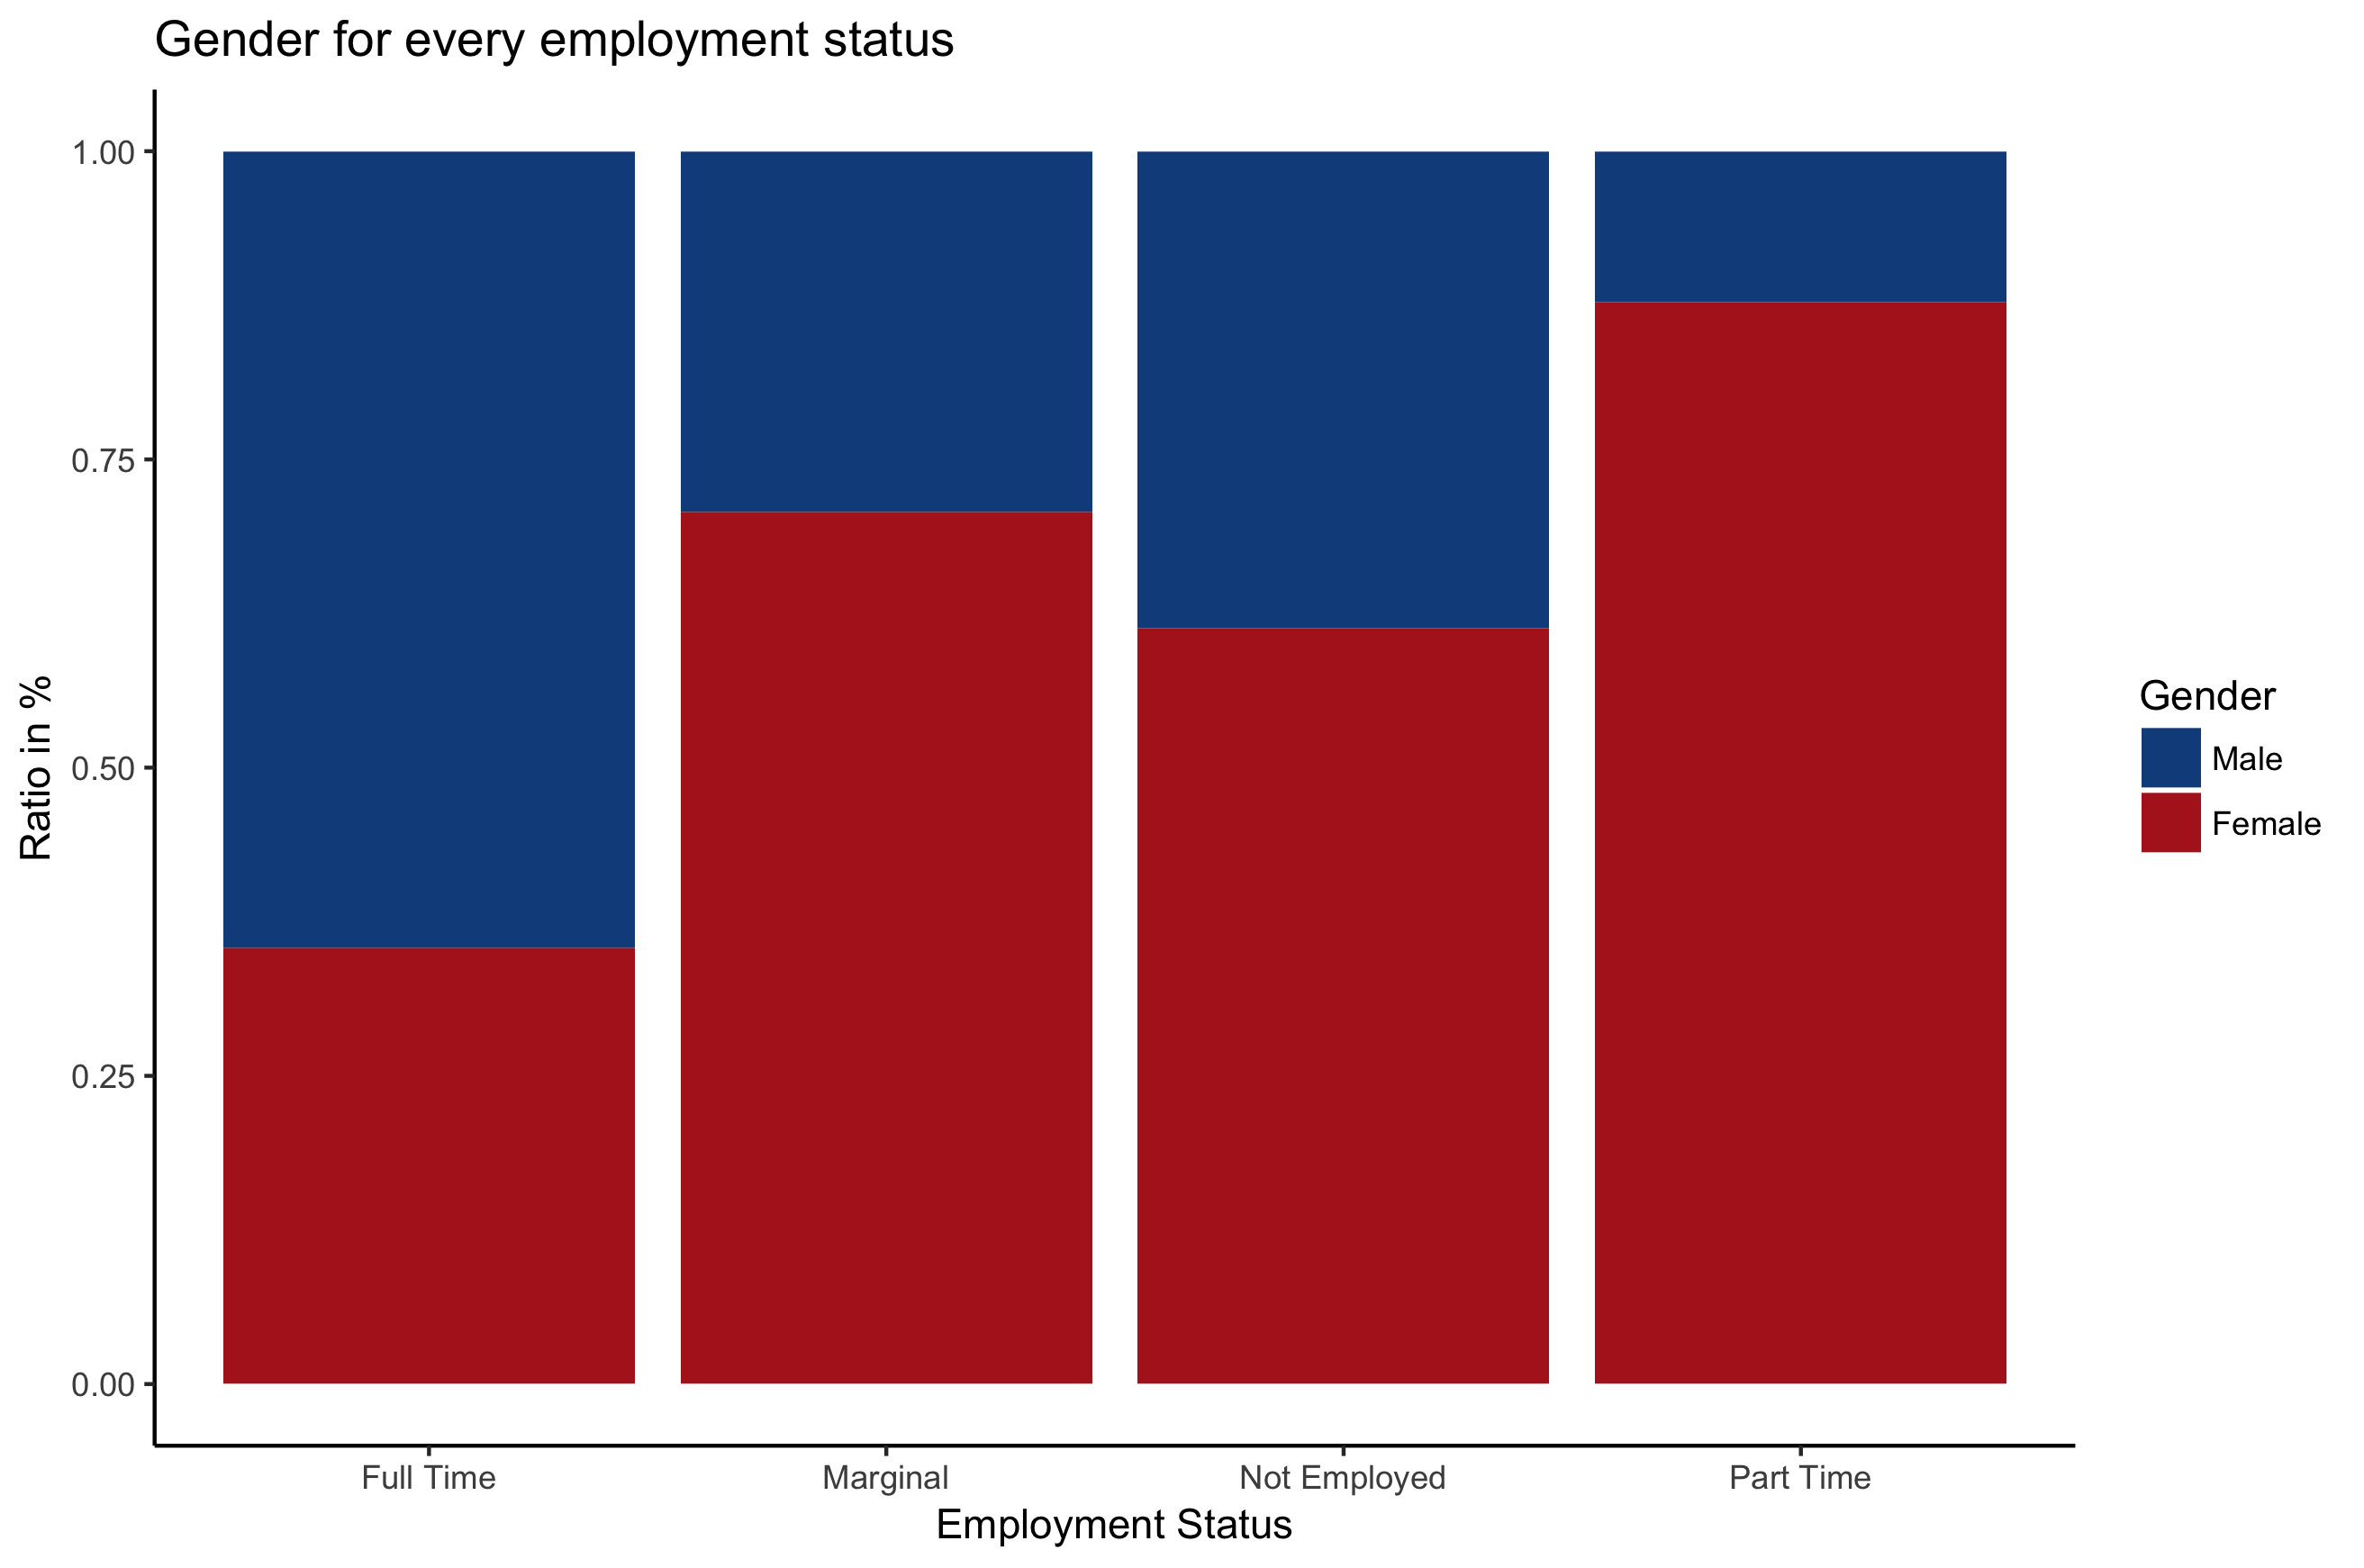
\includegraphics[width=\textwidth]{q2/plot_ouput_gender_employment.png}
\end{figure}

%Figure: 4 Density Plots
\begin{figure}
\caption{Density Plots}
\begin{subfigure}[h]{0.5\linewidth}
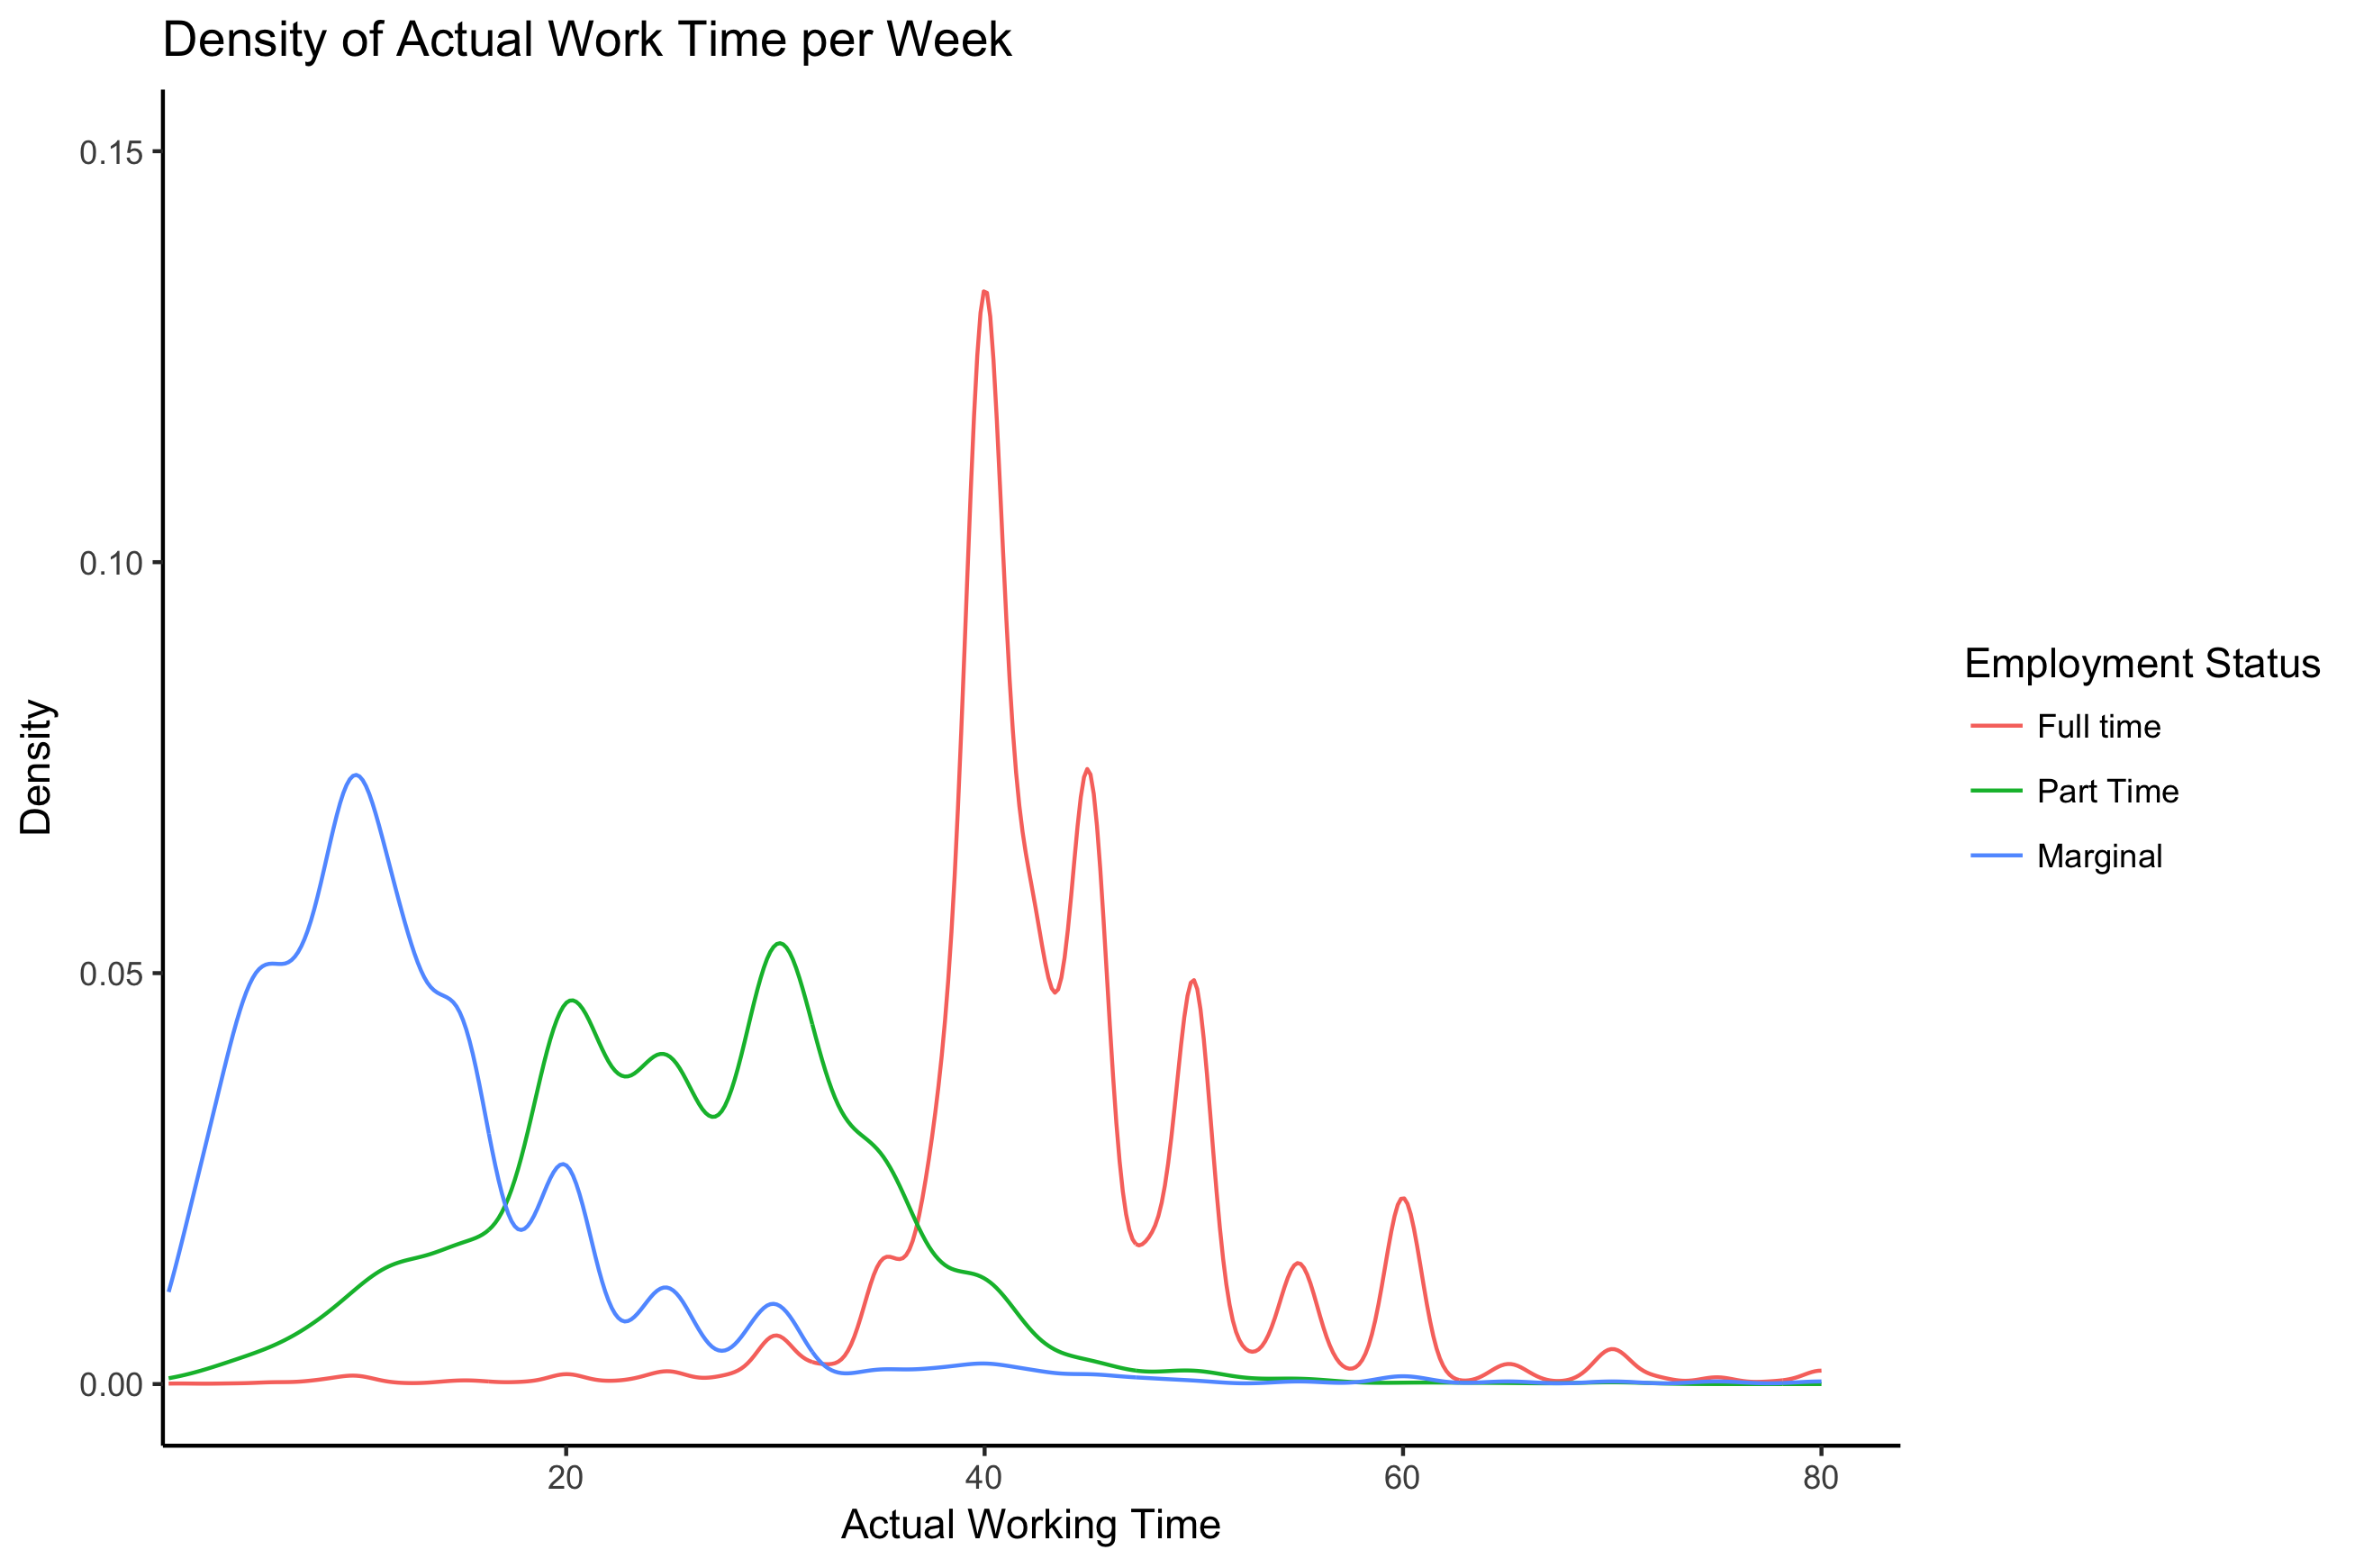
\includegraphics[width=\textwidth]{q2/plot_ouput_density_actual_work.png}
\caption{Density of actual work time per week}
\end{subfigure}
\hfill
\begin{subfigure}[h]{0.5\linewidth}
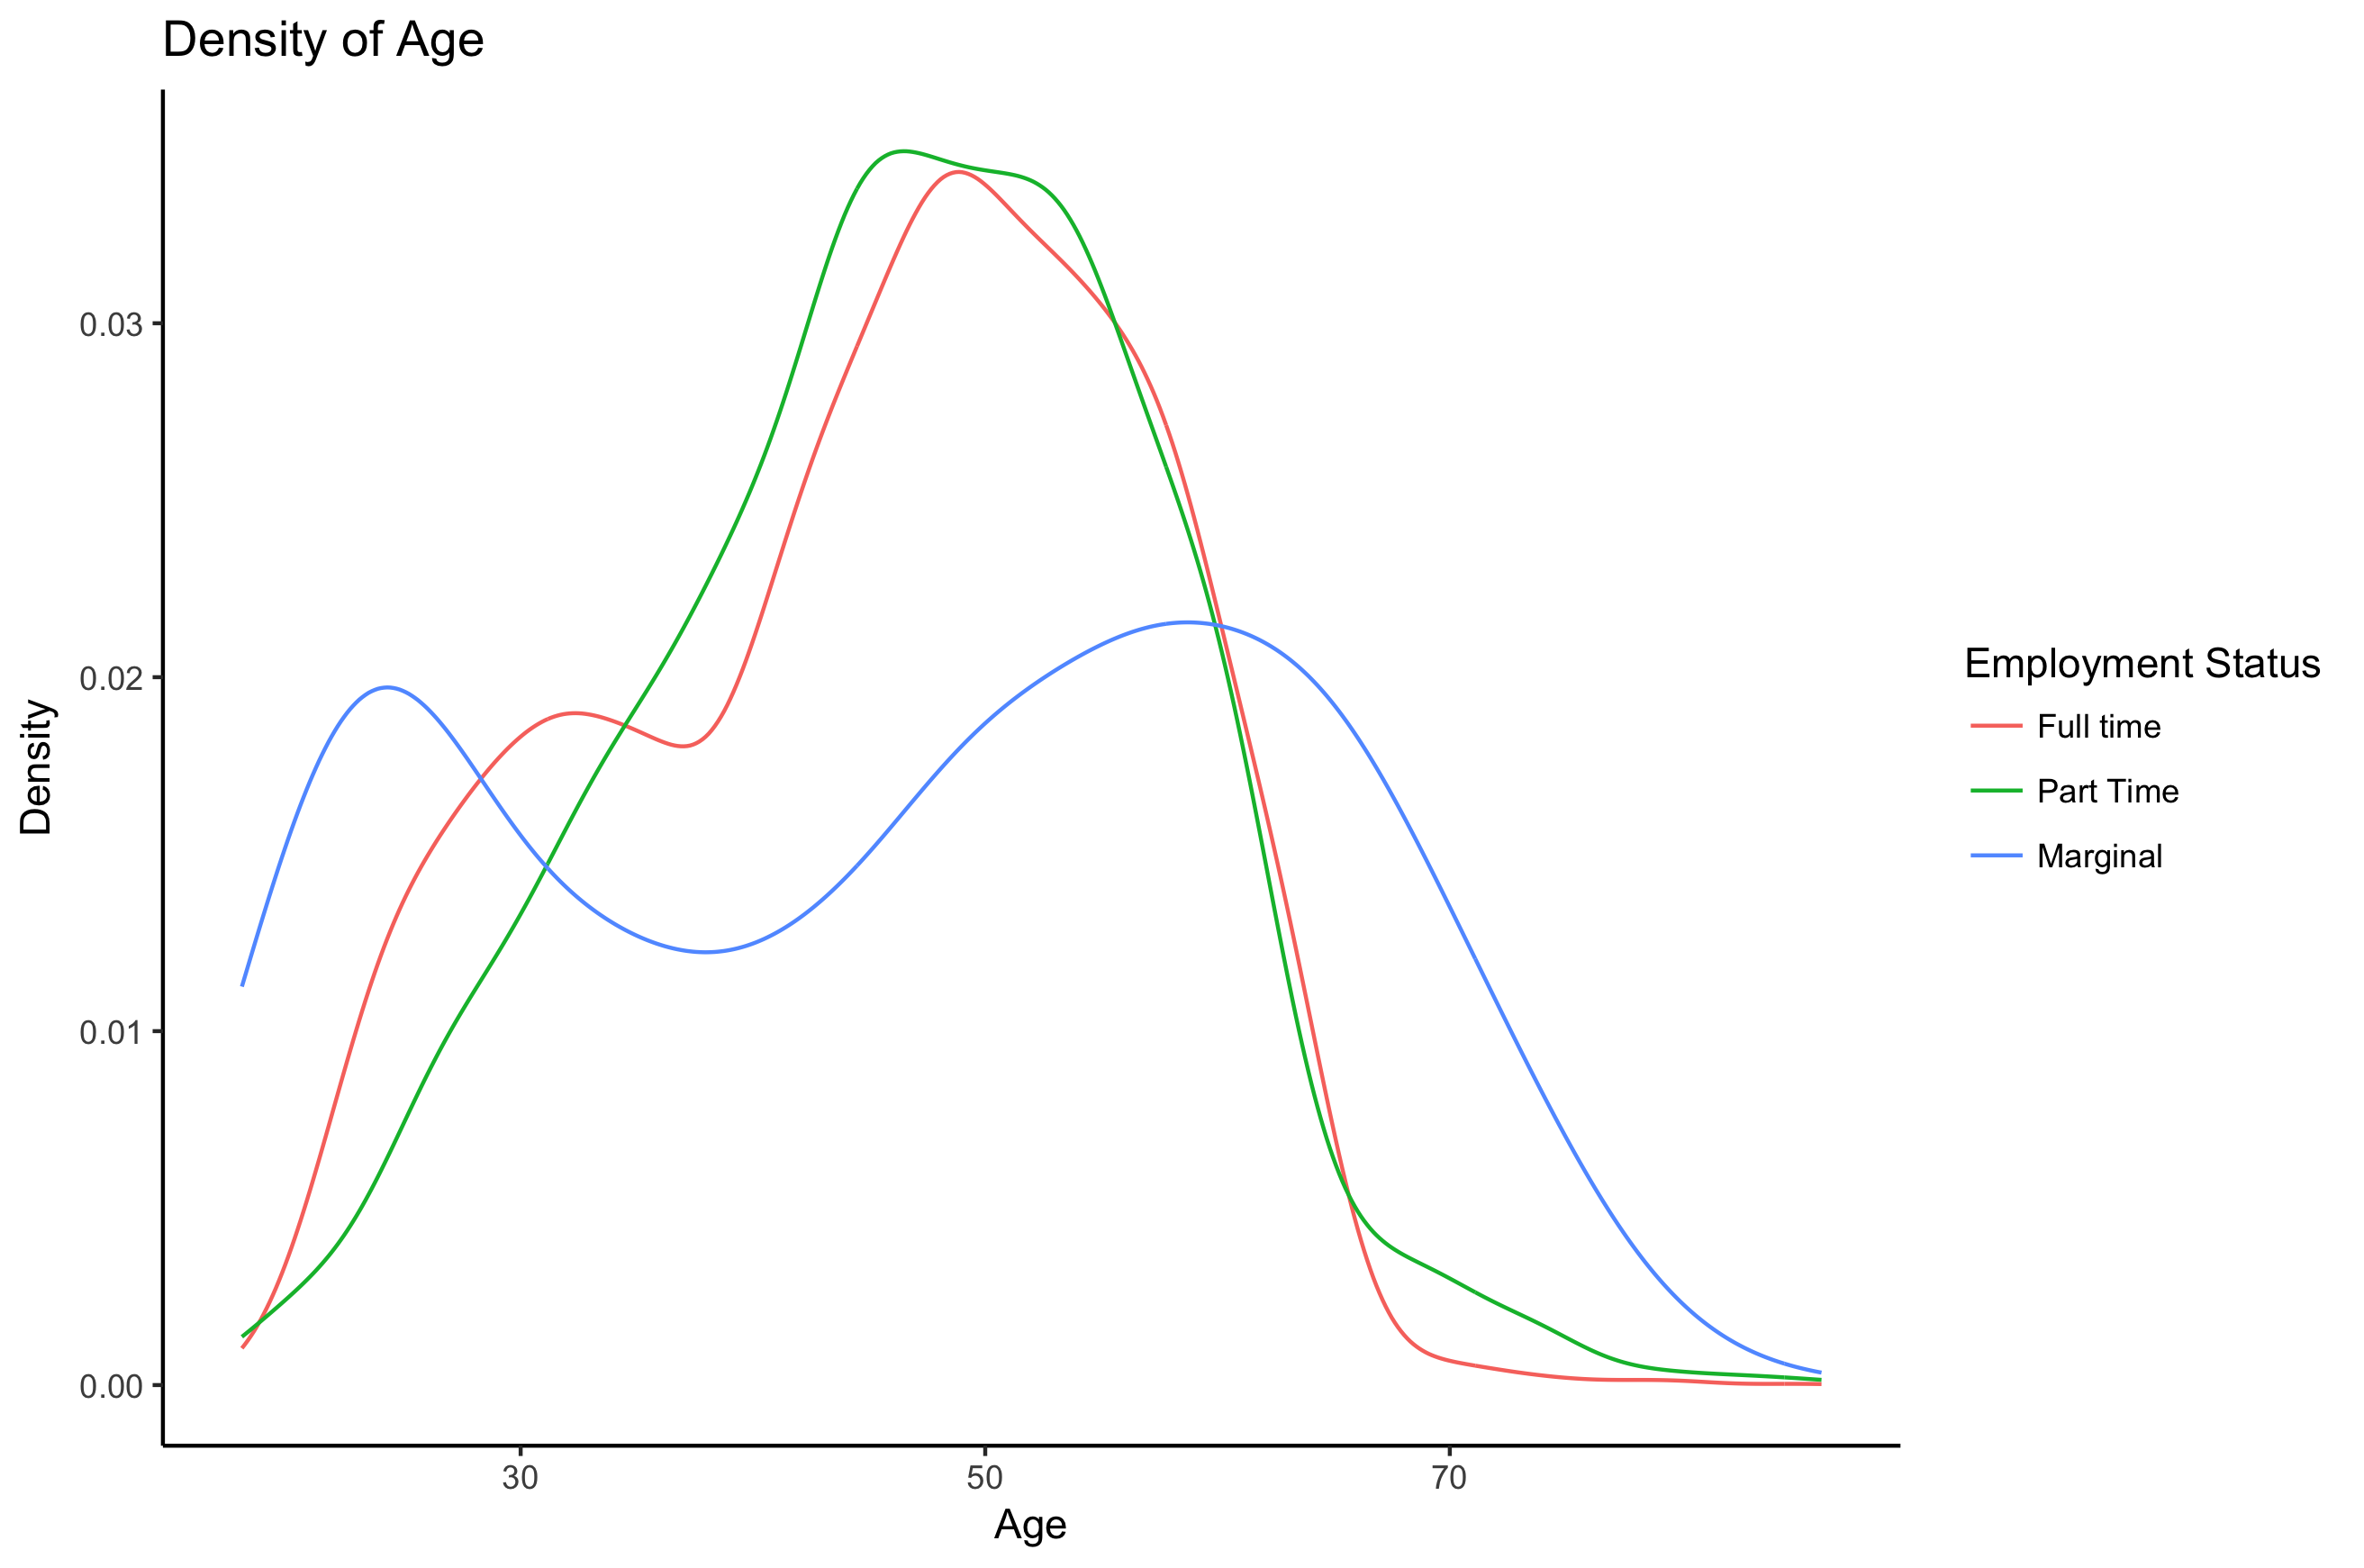
\includegraphics[width=\textwidth]{q2/plot_output_density_age.png}
\caption{Density of Age}
\end{subfigure}
\label{q6m}

\begin{subfigure}[h]{0.5\linewidth}
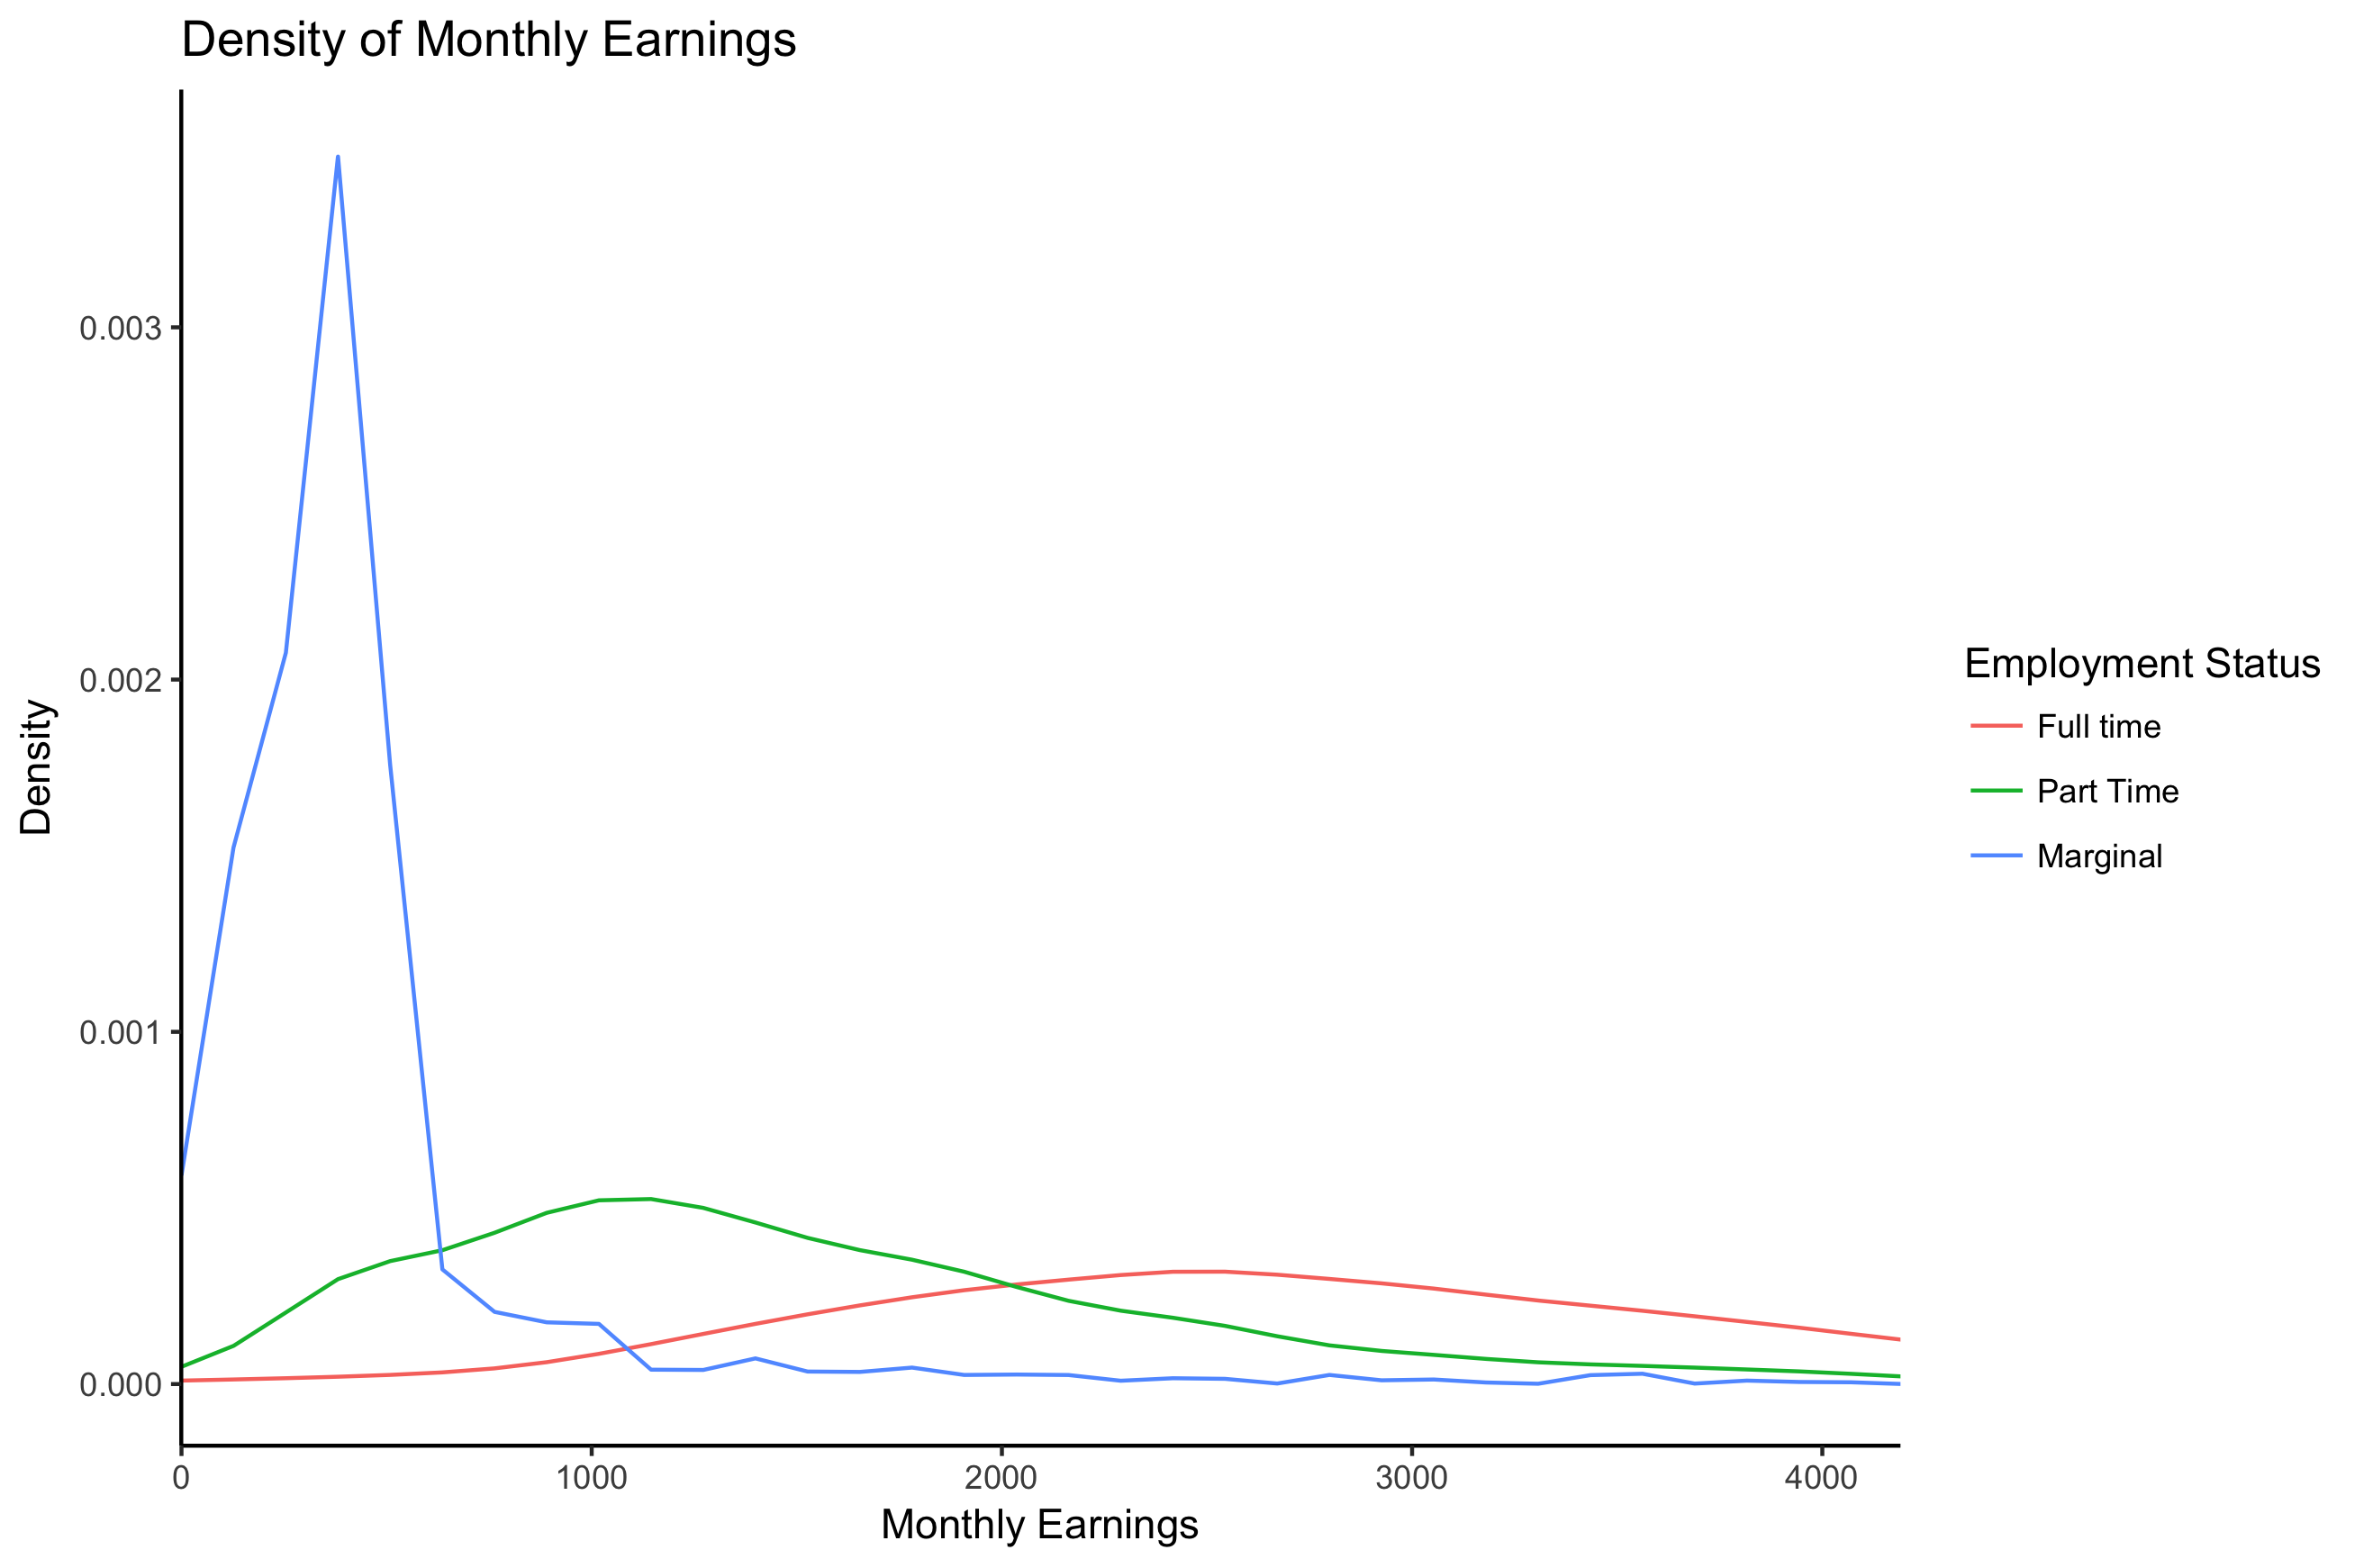
\includegraphics[width=\textwidth]{q2/plot_output_density_monthly_earnings.png}
\caption{Density of monthly earnings}
\end{subfigure}
\hfill
\begin{subfigure}[h]{0.5\linewidth}
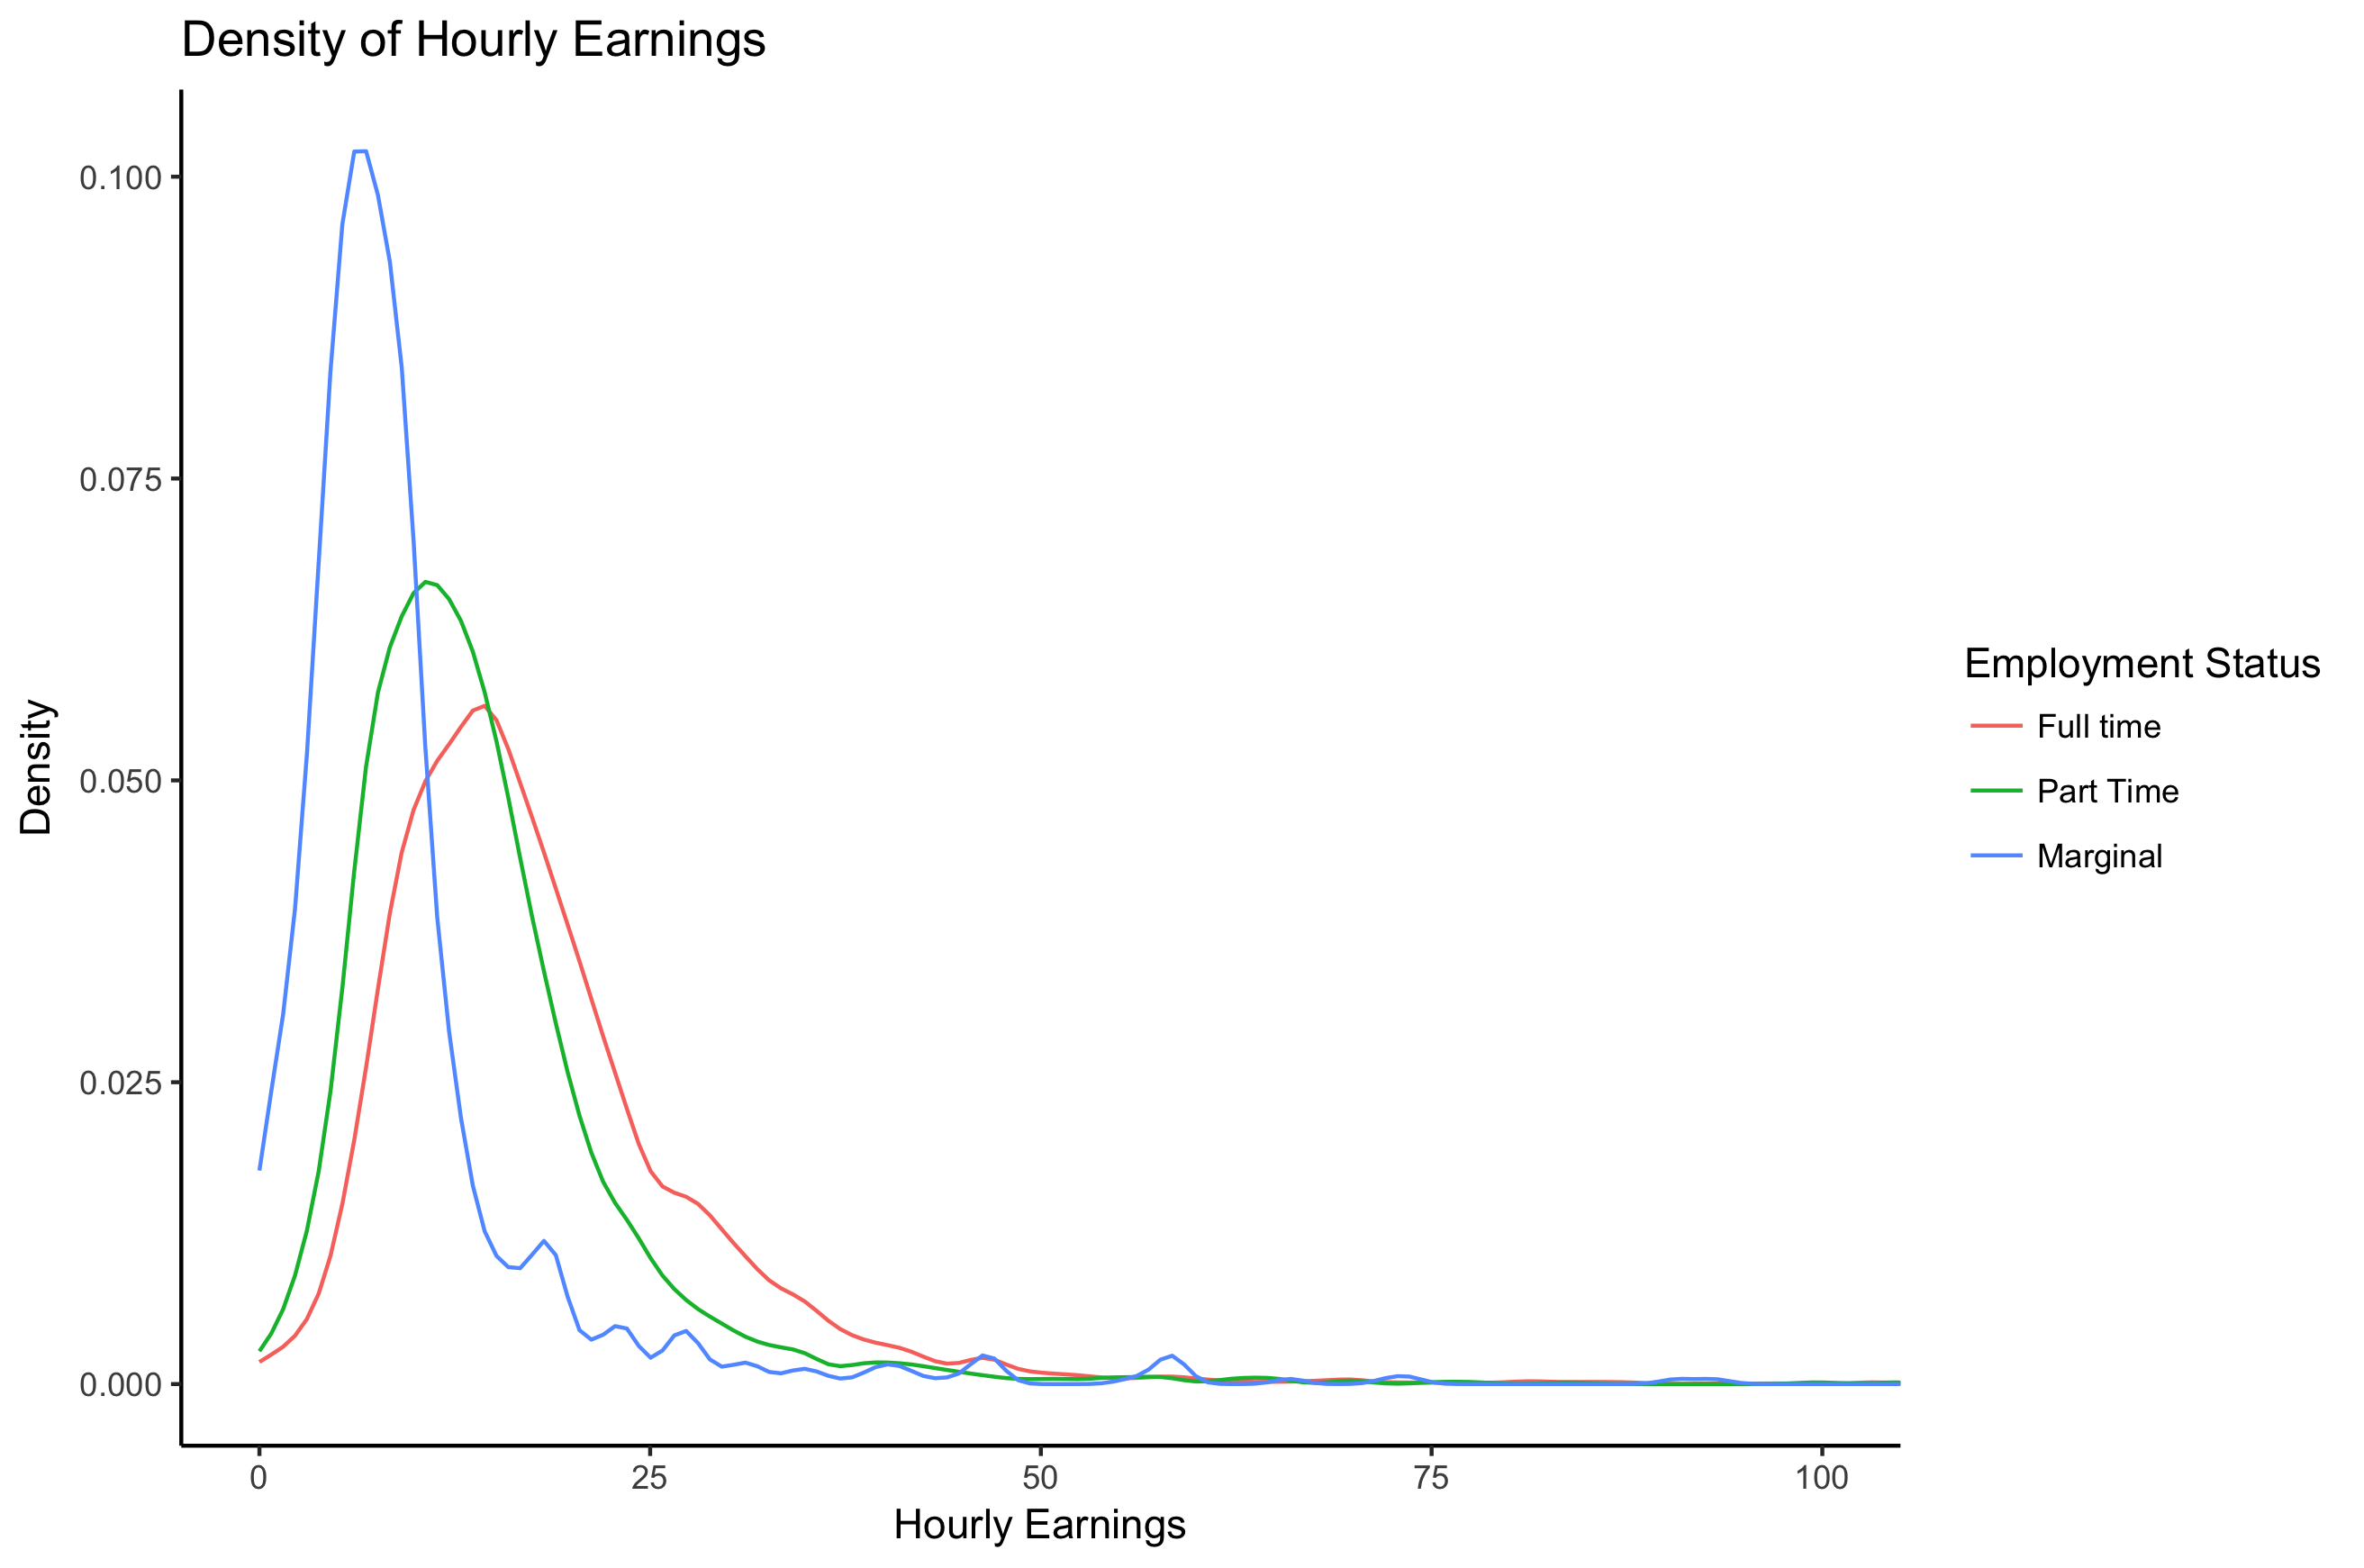
\includegraphics[width=\textwidth]{q2/plot_output_density_earnings.png}
\caption{Density of hourly earnings}
\end{subfigure}%
\label{q6m}
\end{figure}

%%%%% End of section3 %%%%%


\section{Simulation of Minimum Wage Effect}
\subsection{Introduction}
This section simulates the effect an increase in income would have on employment, based on \cite{boll2015potenzielle}. 
For this, it is important to look at two possible labor market models. The first follows the neoclassical approach and the theory of total competition, the second a monopsonic market with only one employer. Is the implemented minimum wage higher than the competition wage but in the range of the marginal productivity of labor there would be a positive effect resulting from the implementation of the minimum wage. Otherwise, there would also be a negative effect. 
Calculating these effects in a simulation can be done with the wage elasticities.   

\subsection{Theory}
Economic theories predict, that in the medium and long term, the low-wage workers would run the risk of being replaced by capital or more highly qualified people if their salaries were increased and thus losing their jobs. Due to simplicity, this model foregoes the possibility of substitution between types of employment and assumes homogeneous production factors. Furthermore, work productivity is constantly modeled, also because it is not possible to model it due to the data. 
In the neoclassical model, companies hire employees until the marginal product of labor equals wages. In contrast, the monopsonist sets a wage below that of the equilibrium, resulting in a loss of wealth, but at a lower cost for the firm. 
The change in employment is given in percent. With $w^{min}$ as the minimum wage, $m$ as the average gross hourly rate and $x$ as the labor demand elasticity.
%Neoclassic formula
\begin{align}
\label{neoclass}
1 - \left(\dfrac{w^{min}}{w}\right)^{-x}
\end{align}
In case there is a monopsonic labor market, the employment effect can be calculated with two alternative formulas, depending on the average wage "$w$" and the market power "$m$".

%monopsonic formula
If $w^{min} > w(1+0.5m)$ use:
\begin{align}
\label{monop}
1 - \left(\dfrac{w^{min}}{w(1+0.5m)}\right)^{-x}
\end{align}

If $w^{min} \leq w(1+0.5m)$ use:
\begin{align}
\label{monop2}
\dfrac{w^{min} - w}{0.5m * w}*1-\left(\dfrac{ 1+0.5m}{1+m}\right)^{-x}
\end{align}
These formulas were also taken from the paper \textit{Potential Effects of a Statutory Minimum Wage on the Gender Pay Gap - A Simulation-Based Study for Germany} written by Boll.
\subsection{Implementation}

Before the models can be used in R, a data frame must be created, that can be used for the models. Here we use the data frame \textbf{sumsub2013} to generate the new \textbf{Affect.by.minwage}.
The average wages for employees affected by minimum wage for each employment status as a new subset are created using the means of important variables. This is again done with the \textbf{dplyr} package and pipe operators.

\begin{lstlisting}
minwage_affect = function(x) {
    x %>% 
    group_by(Employment.Status, Subject.to.minwage) %>% 
#	[SEE ENTIRE SOURCE IN APPENDIX]
}
# Apply Function to create Affected.by.minwage using sumsub2013
Affected.by.minwage = minwage_affect(sumsub2013)
\end{lstlisting}
For the simulation, only the persons affected by the minimum wage are considered. For this, the function \textbf{select\_average\_earnings} filters the dataset  according to those persons, having the value \textit{1} in the variable \textbf{Subject.to.minwage}.
\begin{lstlisting}
select_average_earnings(Affected.by.minwage)
\end{lstlisting}
First of all, a vector is required containing different elasticities for which the values can be calculated from the models later on. This vector can be filled with different values and also independent of the quantity. The following vector includes the five values used in the corresponding paper. However, the vector could also contain more or less, as the source code is created flexibly.
\begin{lstlisting}
Labor.Demand.Elasticity = c(-0.2, -0.5, -0.75, -1, -1.2)
\end{lstlisting}
The neoclassical model (model: \ref{neoclass}) has been implemented in such a way that the number of observable groups can be adjusted. An input data frame and the elasticity vector are required as input. For the output the new values with new names for the columns, which can also be extended in the set of data, are then attached to the data frame of the input. The function \textbf{employ\_effect} calculates the values for \textbf{Neo.Employment.Effect} based on input data and the given elasticities. The column names are generated based on the length of the elasticity vector and the \textit{paste}-function (in this case, 1-5).
%model neoclassic
\begin{lstlisting}
employ_effect = function(x, y) {
    for (list in 1:length(x)) {
        curr_col = 1 - (8.5/y$avg_Hourly.earnings)^(-1 * x[list])
        y[, paste("Neo.Employment.Effect", list, sep = "")] = curr_col
    }
    return(y)
}

# Apply the employ_effect function for the dataset used before
Affected.by.minwage = \\
	employ_effect(Labor.Demand.Elasticity, Affected.by.minwage)
\end{lstlisting}
The following function \textbf{employ\_effect\_monopsonic} calculates the values for the monopsonistic model. It takes different input data: again, the labor demand elasticities and the preprocessed SOEP-data as well as a market power, which may vary over time. In the current case, it is assumed that the market power is set to 0.2. First, the function creates an empty data frame and new column names with the \textbf{paste}-function like in the step before. Again, the number of columns corresponds to the length of the elasticity vector. A new column \textbf{NewWage} is then calculated. These values are used as decision criteria for selecting the respective calculation method. Which of the two formulas explained above is used for the calculation is checked by if-condition, as the model changes when the minimum wage is less than the wage weighted by the monopsonist's market power. The function decides separately for each row of the data frame which formula is used and then calculates a value for each value in the elasticity vector, which is inserted in the corresponding columns. After each iteration, the current row gets appended to the formerly created data frame \textbf{effect\_matrix} with \textbf{rbind}. Like in the function for the neoclassic model, the new values with new names for the columns, which can also be extended in the set of data, are then attached to the data frame with \textbf{cbind}. That data frame is the same as in the function before and is extended by the new values created in this function. Everything is dynamic and can be extended with additional data. 
%model monopsonic
\begin{lstlisting}
employ_effect_monopsonic = function(x, y, m) {
    new_cols = paste("Mon.Employment.Effect", 1:length(x), sep = "")
    effect_matrix = as.data.frame(matrix(ncol = length(x)))
    effect_matrix = effect_matrix[FALSE, ]
    y$NewWage = y$avg_Hourly.earnings * (1 + 0.5 * m) 
    for (lines in 1:nrow(y)) {
        if (8.5 > y$NewWage[lines]) {
            curr_row = 1 - \\
            	(8.5/(y$avg_Hourly.earnings[lines] * (1 + m)))^(-x)
            effect_matrix = rbind(effect_matrix, curr_row)
        } else {
            curr_row = ((8.5 - y$avg_Hourly.earnings[lines])/ \\
            	(0.5 * m * y$avg_Hourly.earnings[lines])) * \\
                (1 - ((1 + 0.5 * m)/(1 + m))^(-x))
            effect_matrix = rbind(effect_matrix, curr_row)
        }
    }
    names(effect_matrix) = new_cols 
    paste("Mon.Employment.Effect", 1:length(x), sep = "")
    output_matrix = cbind(y, effect_matrix) 
    return(output_matrix)
}

# Apply the employ_effect_monopsonic function for the dataset \\
# used the function before with market power of 0.2
Affected.by.minwage = employ_effect_monopsonic \\
	(Labor.Demand.Elasticity, Affected.by.minwage, 0.2)
\end{lstlisting}
To illustrate the results properly, the data of the neoclassical model are visualized using the \textbf{ggplot2}-package. The function \textbf{plot\_graph\_effect\_minwage} is used for this purpose and takes the preprocessed SOEP-data as well as the elasticities as input data. First, the values of the neoclassical model were selected in a new data frame and the matrix is transposed afterwards. Then, the graphs are created for the corresponding groups with the increasing elasticity values shown on the X-axis and the negative values of the change in employment can be found on the Y-axis. This is used as negative values because it is more properly suited for illustrative purposes. The function gets applied with the input data mentioned above and creates the desired plot.
%plot simulation
\begin{lstlisting}
plot_graph_effect_minwage = function(input, elasticities) {
    dens1 = input %>% 
    select(Employment.Status, Neo.Employment.Effect1, \\
    Neo.Employment.Effect2, Neo.Employment.Effect3, \\
    Neo.Employment.Effect4, Neo.Employment.Effect5) 
    tdens1 = as.data.frame(t(dens1))
    colnames(tdens1) = c("fulltime", "parttime", "marginal")
    tdens1 = tdens1[-1, ]
    tdens1$elast = elasticities
    tdens1$fulltime = as.numeric(as.vector(tdens1$fulltime))
    tdens1$parttime = as.numeric(as.vector(tdens1$parttime))
    tdens1$marginal = as.numeric(as.vector(tdens1$marginal))
#    [GGPLOT-PART SEE APPENDIX]
\end{lstlisting}

\subsection{Output}
The data from the simulations always show a negative trend. Therefore, an increase in wages would always lead to a reduction in incomes of employees. This is due to the choice of individuals. Since at the beginning we only chose the individuals who are affected by the minimum wage. The graph (Figure \ref{simu}) shows that with increasing elasticity, the number of people falling into unemployment increases. Since the change in employment reacts more strongly to the change in wages with increasing elasticity values. The change among full-time employees is always the lowest. Part-time employees have slightly larger differences and the marginal ones have a much larger change in their employment, with rising wages. In the neoclassical model, the values are always given the same elasticity and employment group as in the monopsonistic model. Here, the first case (model \ref{monop2}) has always occurred in the monopsonistic model. Since the minimum wage is always higher than the average wage weighted by market power. The values are significantly lower than those in the comparative paper, but show a similar trend given the values. Values that better reflect reality should always lie between the values of the two models, since in reality none of these models can be assumed. But the behaviour of the monopsonist can also be seen as the behaviour of the worker, who for irrational reasons or heterogeneous preferences does not quit his job just because he has not received an adequate salary increase. Also like the neoclassical model, nobody would directly quit their job just only by the reason they now earn one cent less. But the model's competition applies to the market and makes it difficult for companies within the company to reduce wages in the long term. We cannot exclute the possibility that there may be no differences in productivity between the groups that could influence the results. But in general, the simulation shows a small but negative trend, which is on average higher for people who work fewer hours. 
%Graph simulation
\begin{figure}[h]
\caption{Simulation of Minimum Wage on Employment}
\label{simu}
\centering
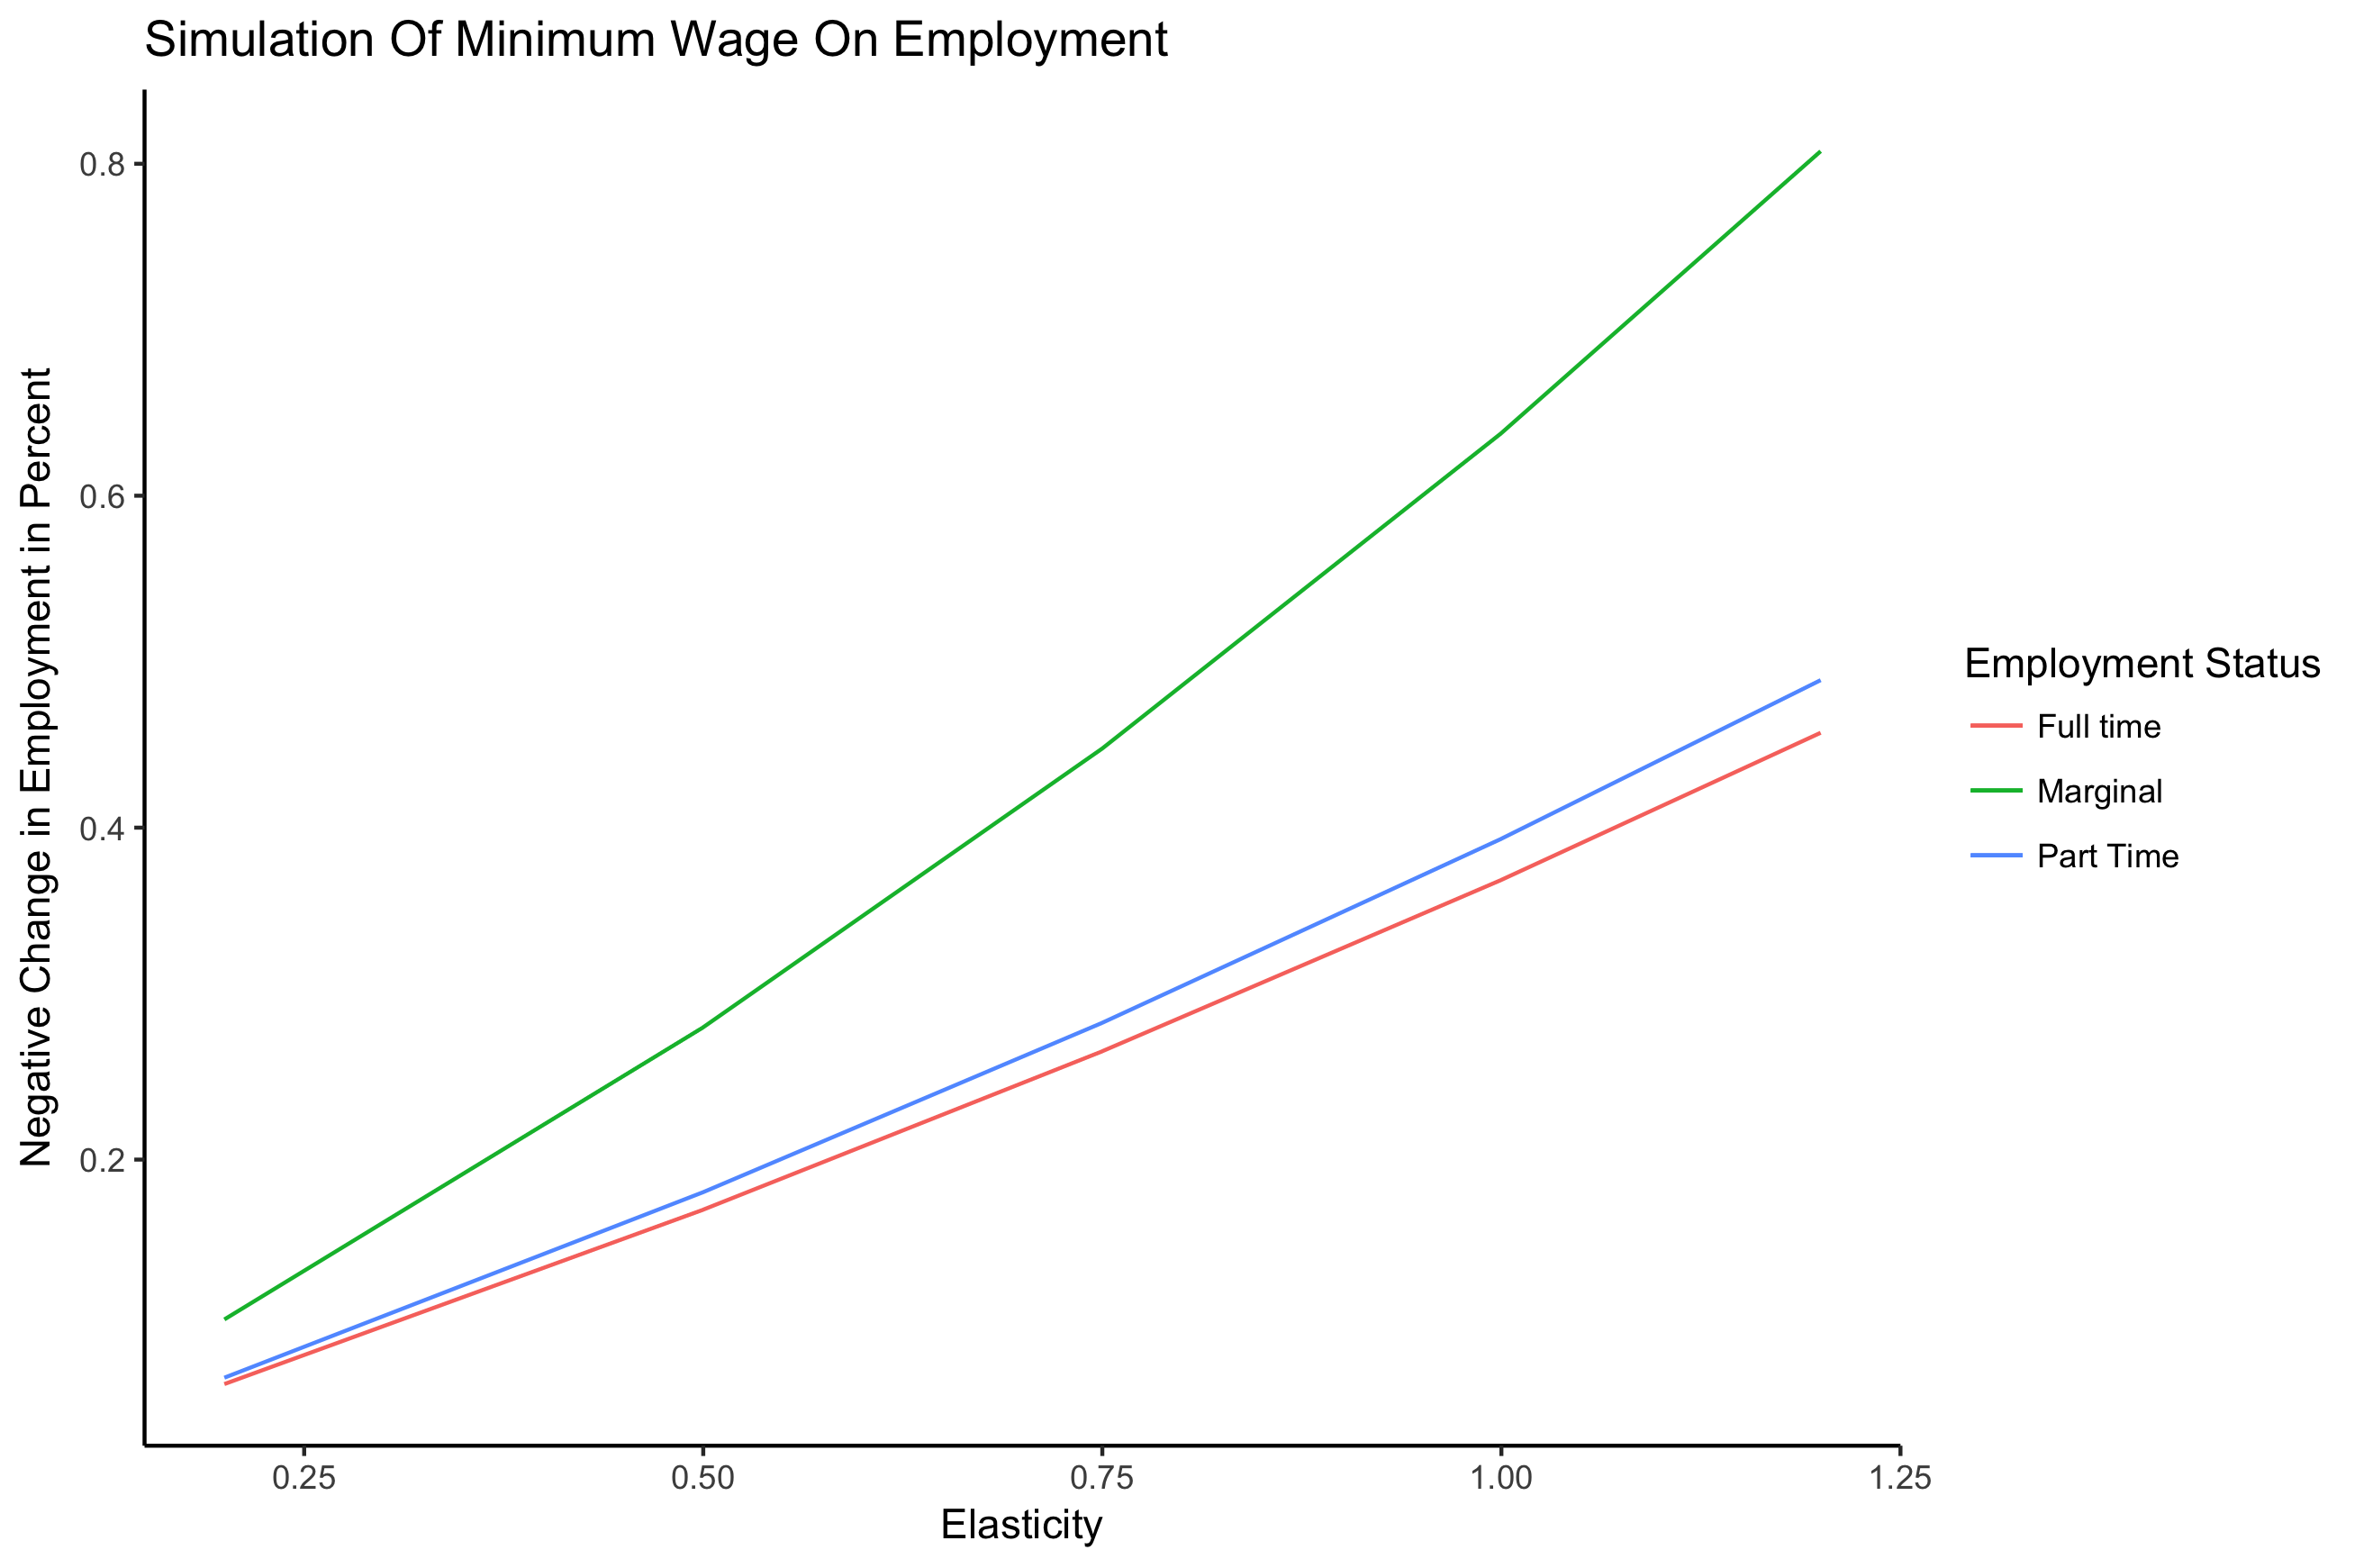
\includegraphics[width=0.75\textwidth]{q3/plot_graph_effect_minwage_output.png}
\end{figure}

%%%%% End of section4 %%%%%

\section{Emplyoment Analysis}
\subsection{Introduction}
In this section an overview of the change of different employment status, over time, is given. People in the SOEP-dataset provide information if they are either \textit{full time employed}, \textit{part time employed}, \textit{marginal employed} or \textit{not employed}. These information are used to see how the employment in Germany overall develops over time. 

\subsection{Theory}
To check for time differences in the full/part/marginal/not employment group different economic measures are used: 
\begin{align}
\ ln(Y_t)
\end{align}
This is the first formula, also worked with in the R where it is called \textbf{Log.Full.Employment.Rate} respectively full can be substituted with other employment status. 

\begin{align}
ln(\Delta Y_t)=ln(Y_t)-ln(Y{t-1})
\end{align}
The logarithmized percentage change of the employment is useful to compress the data and get the standard distribution. This makes the graph more vivid and meaningful. In the code this value is labeled as \textbf{Delta.Log.Full.Employment} and also used for the other employment status.  

\begin{align}
\dfrac{Y_t}{N_t}\equiv y_t
\end{align}
This formula gives the employment rate, named \textbf{Full.Employment.Rate} in the code, for every year. It can be adapted for all four groups of employment status, as well. 

\begin{align}
ln(\dfrac{Y_t}{N_t})= ln(y_t)
\end{align}
The logarithmized employment rate of full/part/marginal/not employment status is given by this formula and is referred to as \textbf{Log.Full.Employment.Rate}, adaptable for all employment status in the code. 

\subsection{Implementation}
Starting out with date pre-processing for the upcoming analysis a dataset only with variables of interest is created by applying the \textbf{data\_selector}-Function, which takes use of the \textbf{dplyr}-package. For the identification of the affected regions variables of interest consist information about employment, the state of residence (which will be assumed to be also most likely the state of working) and information about the income. The new dataset is called \textbf{Reduced\_merged}.
\begin{lstlisting}
data_selector = function(merged_all) {
    select(filter(merged_all), c(Wave, never.Changing.Person.ID, 
    State.of.Residence, Employment.Status, Labor.Force.Status, 
    Actual.Work.Time.Per.Week, Current.Gross.Labor.Income.in.Euro))
}
Reduced_merged = data_selector(merged_all)
\end{lstlisting}

To work with the newly created data frame more efficiently, some variables have to be adjusted. In the \textbf{Labor.Force.Status}-variable, people who do not work anymore are sorted out, likewise people who are too old and therefore do not work any more as well. The function \textbf{adj\_labor\_force} is then applied to the \textbf{Reduced\_merged} dataset.
With the same procedure, the variables \textbf{Work.Time} and \textbf{Gross.Labor.Income} are modified later on. 
\begin{lstlisting}
adj_labor_force = function(x) {
    x$LaborForce_num = NA
    x$LaborForce_num = as.numeric(x$Labor.Force.Status)
    x$LaborForce_num[x$LaborForce_num <= 6] = NA
    x$LaborForce_num[x$LaborForce_num == 8] = NA
    return(x)
}
Reduced_merged = adj_labor_force(Reduced_merged)
\end{lstlisting}

In the next step, all rows in the dataset having at least one \textit{NA}-value are dropped. Thus, a function is created and applied to the \textbf{Reduced\_merged} dataset. Only complete rows remain in the dataset \textbf{Reduced\_merged\_noNA}. 
\begin{lstlisting}
drop_sub_na = function(x) {
    x[complete.cases(x), ]
}
Reduced_merged_noNA = drop_sub_na(Reduced_merged)
\end{lstlisting}

To show all observations of each employment status for each year, the function \textbf{yearly\_-employment} below is created. 
The function gets applied to the \textbf{Reduced\_merged\_noNA} dataset. 
Similarly, the function \textbf{yearly\_employment\_state} is created. This function provides a view on the dataset grouped by state of residence and wave. Both can be found within the source code in the appendix.
\begin{lstlisting}
yearly_employment = function(x) {
x %>% group_by(Wave) %>% summarise(Observations = n(), 
Full.Employment=length(Employment.Status[as.numeric(Employment.Status)==7]), 
#	[OTHER EMPLOYMENT STATUSES SEE APPENDIX]
}
Employment.yearly = yearly_employment(Reduced_merged_noNA)
\end{lstlisting}

The following function \textbf{calc\_employment\_variables} generates the four different employment measures developed in the previous theory section. It consists of four parts, one for every employment status. It can be used for any employment status defined by SOEP, which are \textit{Full Time}, \textit{Part Time}, \textit{Marginal} and \textit{Not Employed}. For each employment status, the function has to be executed once by indicating the input data and the employment type. An if statement checks the respective employment status and executes the corresponding area. If an invalidity employment status is specified, the program throws an error. The following source code again represents only a part of the entire code, which can be found in the appendix.
\begin{lstlisting}
calc_employment_variables = function(input, type) {
  if (type == "Full") {
  input$v1 = log(input$Full.Employment)
  input$v2 = c(0, diff(input$v1))
  input$v3 = (input$Full.Employment/input$Observations) * 100
  input$v4 = log(input$v3)
  colnames(input)[colnames(input) == "v1"] = "Log.Full.Employment"
  colnames(input)[colnames(input) == "v2"] = "Delta.Log.Full.Employment"
  colnames(input)[colnames(input) == "v3"] = "Full.Employment.Rate"
  colnames(input)[colnames(input) == "v4"] = "Log.Full.Employment.Rate"
  # [REMAINING PART SEE APPENDIX]
  } else {
     print("Error! Input must either be Full, Part, Marginal or Not")
    }
    return(input)
}
\end{lstlisting}

The formerly created function \textbf{calc\_employment\_variables} gets applied to the datasets \textbf{Employment.yearly} and \textbf{Employment.state}. This is done for each employment status separately. The following code only shows the case of full employment using the \textbf{Employment.yearly}-dataset. The other parts can be found in the appendix.
\begin{lstlisting}
Employment.yearly = calc_employment_variables(Employment.yearly, "Full")
\end{lstlisting}

The SOEP data set conducts data over a period of one year. To make it clear, especially in the following graphs, that the data is panel data and observes a period of time, it is necessary to apply the newly created function \textbf{create\_period}. It generates periods for every year in \textbf{list\_years} by counting every year one up and pasting each of them together. The function is then applied to the objects used above by creating a new column in each dataset.
\begin{lstlisting}
create_periods = function(list_years) {
    list_years_up = as.numeric(list_years) + 1
    list = paste(list_years, list_years_up, sep = "/")
    return(list)
}
Employment.yearly$Period = create_periods(list_years)
Employment.yearly.state$Period = create_periods(list_years)
\end{lstlisting}
%
\subsection{Output}
To make use of the new variables graphically \textbf{ggplot2} is used. First, we visualize the different kind of employment measures for the separate employment statuses of time.
%
\begin{figure}
\caption{Employment measures}
\begin{subfigure}[h]{0.5\linewidth}
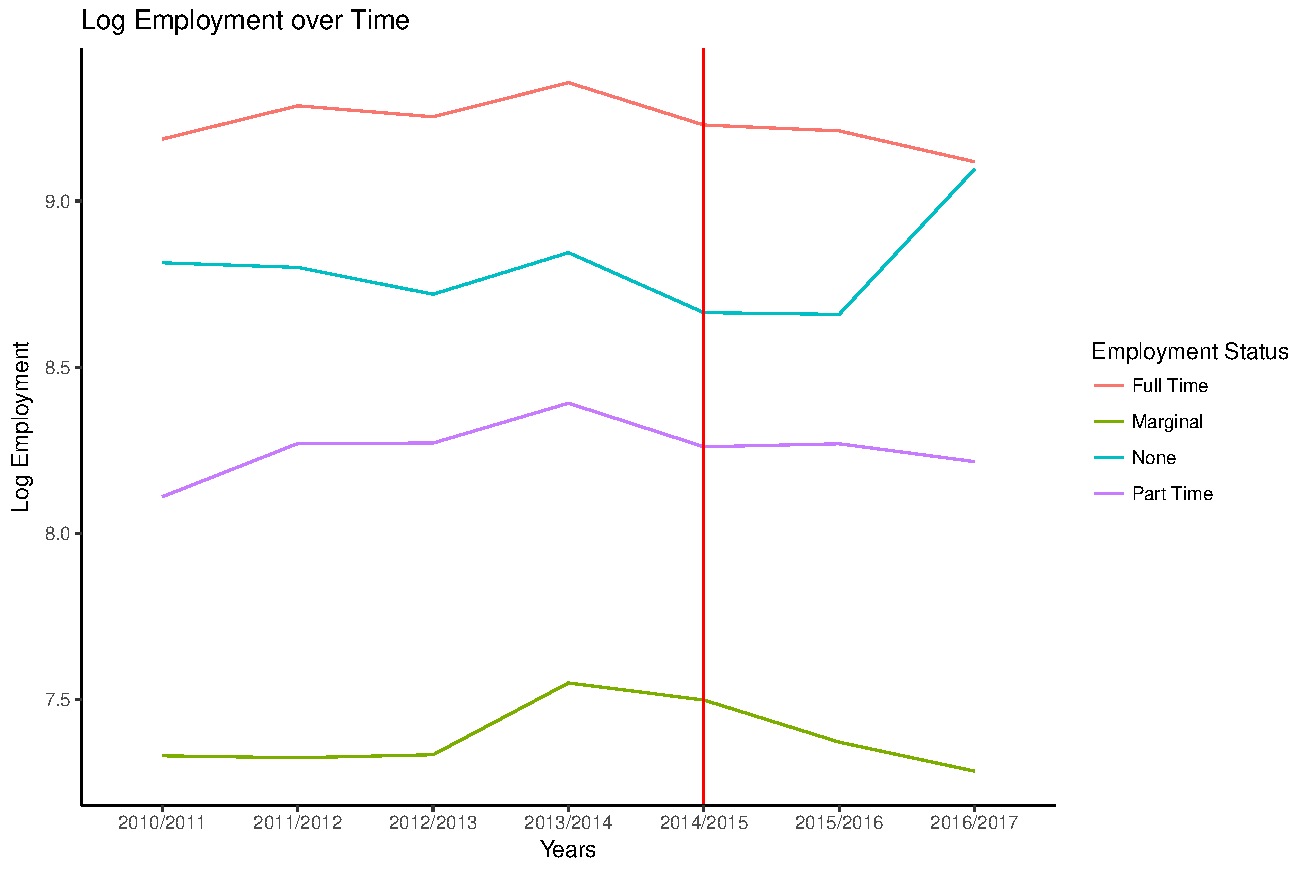
\includegraphics[width=\textwidth]{q4/yearlog.pdf}
\caption{Log Employment}
\end{subfigure}
\hfill
\begin{subfigure}[h]{0.5\linewidth}
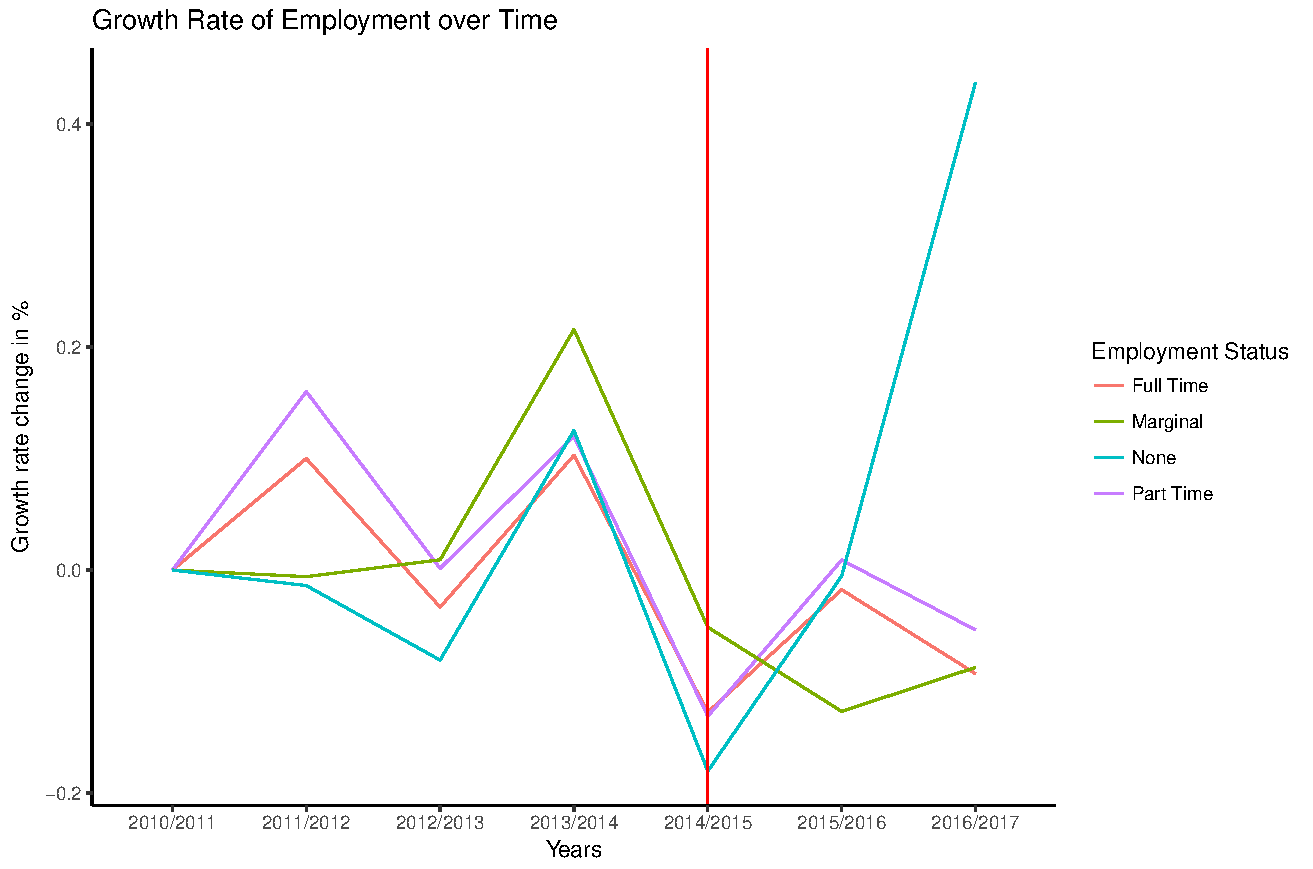
\includegraphics[width=\textwidth]{q4/yearchangelog.pdf}
\caption{Change of Log Employment}
\end{subfigure}

\begin{subfigure}[h]{0.5\linewidth}
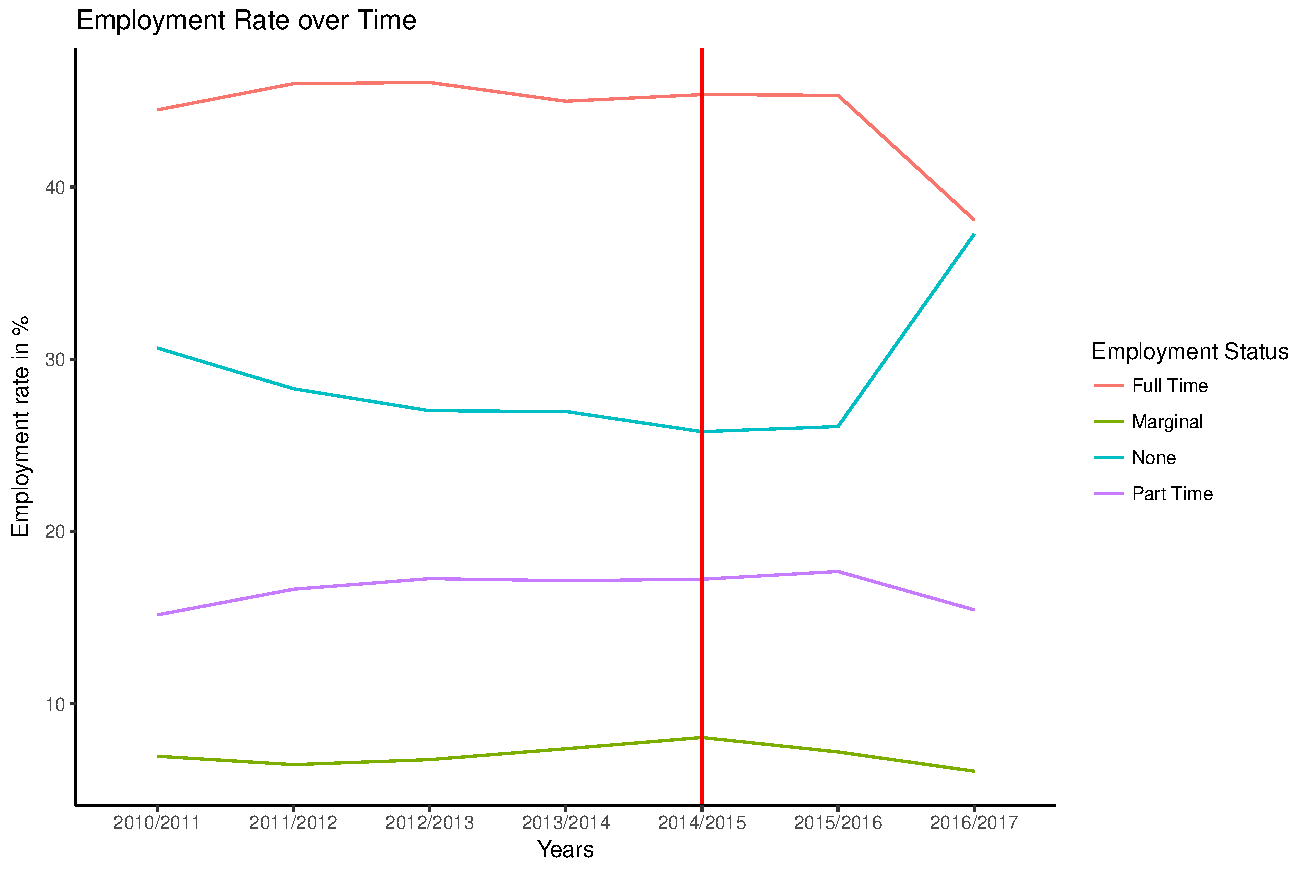
\includegraphics[width=\textwidth]{q4/yearemployrates.pdf}
\caption{Share of Employment}
\end{subfigure}
\hfill
\begin{subfigure}[h]{0.5\linewidth}
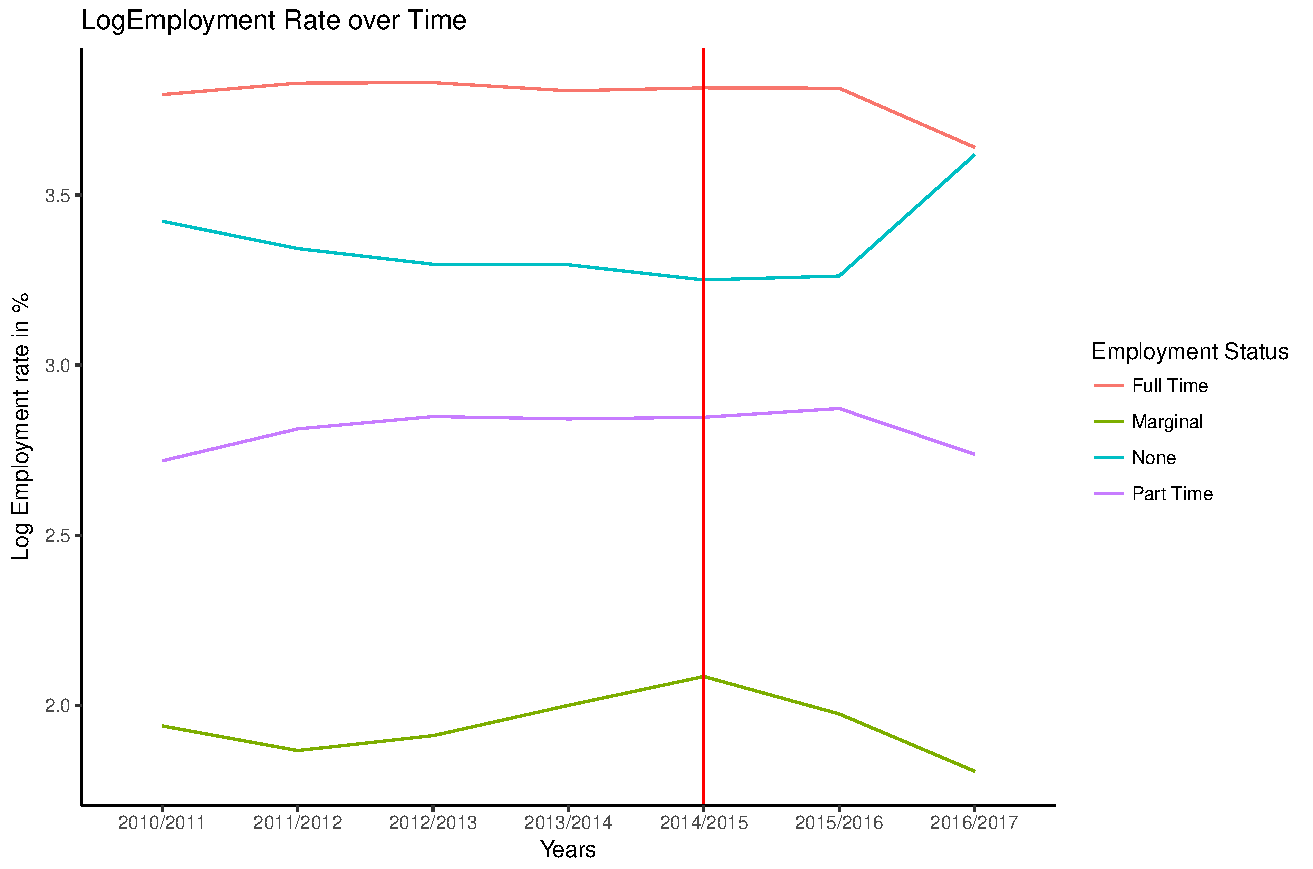
\includegraphics[width=\textwidth]{q4/yearlogemployrates.pdf}
\caption{Log Growth Rate Employment}
\end{subfigure}%
\label{q4graph1}
\end{figure}
%
%
Figure \ref{q4graph1} displays four different measures, the log employment (a), the change of the log employment (b), the share of employment (c) and the log share of employment(d). In all four graphs the trend is rather similar. After the introduction of the minimum wage, which is highlighted by the red marker, all employment groups shrink, except the non employment line, which rises naturally. Interestingly, there appears to be a drop in employment for all groups before the minimum wage introduction as figure \ref{q4graph1} (a) indicates. Figure \ref{q4graph1} (b) indicates the dynamics of the change of the log employment value. It appears, that before the minimum wage introduction the employment statuses move rather similar however there is a discrepancy afterwards, with the huge increase of the non-employment group. This, of course, depends on  the increase in (a). Figure \ref{q4graph1} (c) and (d) are very similar, which makes perfect sense as (d) is a logarithmic transformation of (c). All in all, this indicates a drop in employment, for all employment status in Germany subsequent to the minimum wage introduction.
%
% 
\begin{figure}
\caption{Share of employment for each state over time}
\begin{subfigure}[h]{0.5\linewidth}
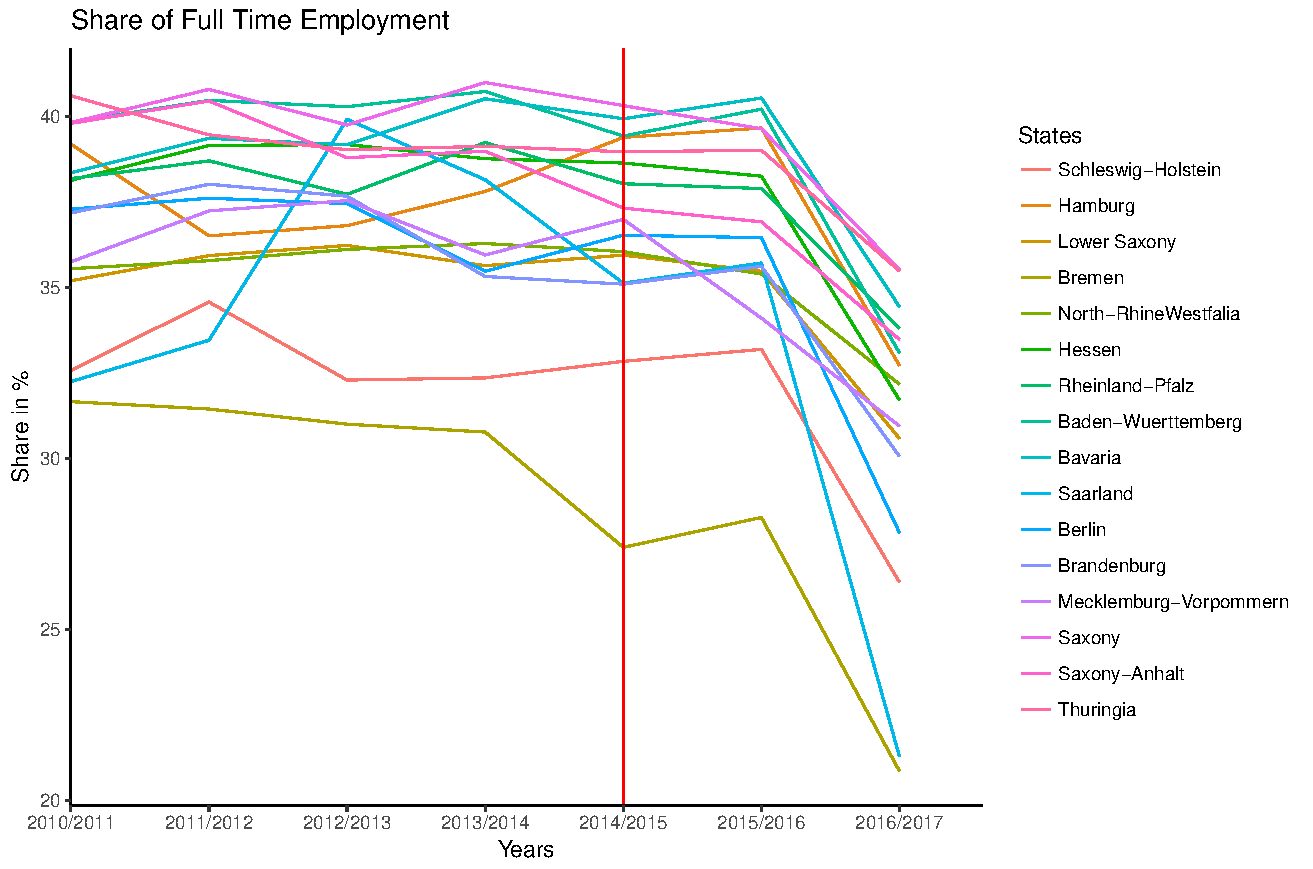
\includegraphics[width=\textwidth]{q4/growthfull.pdf}
\caption{Full time employment}
\end{subfigure}
\hfill
\begin{subfigure}[h]{0.5\linewidth}
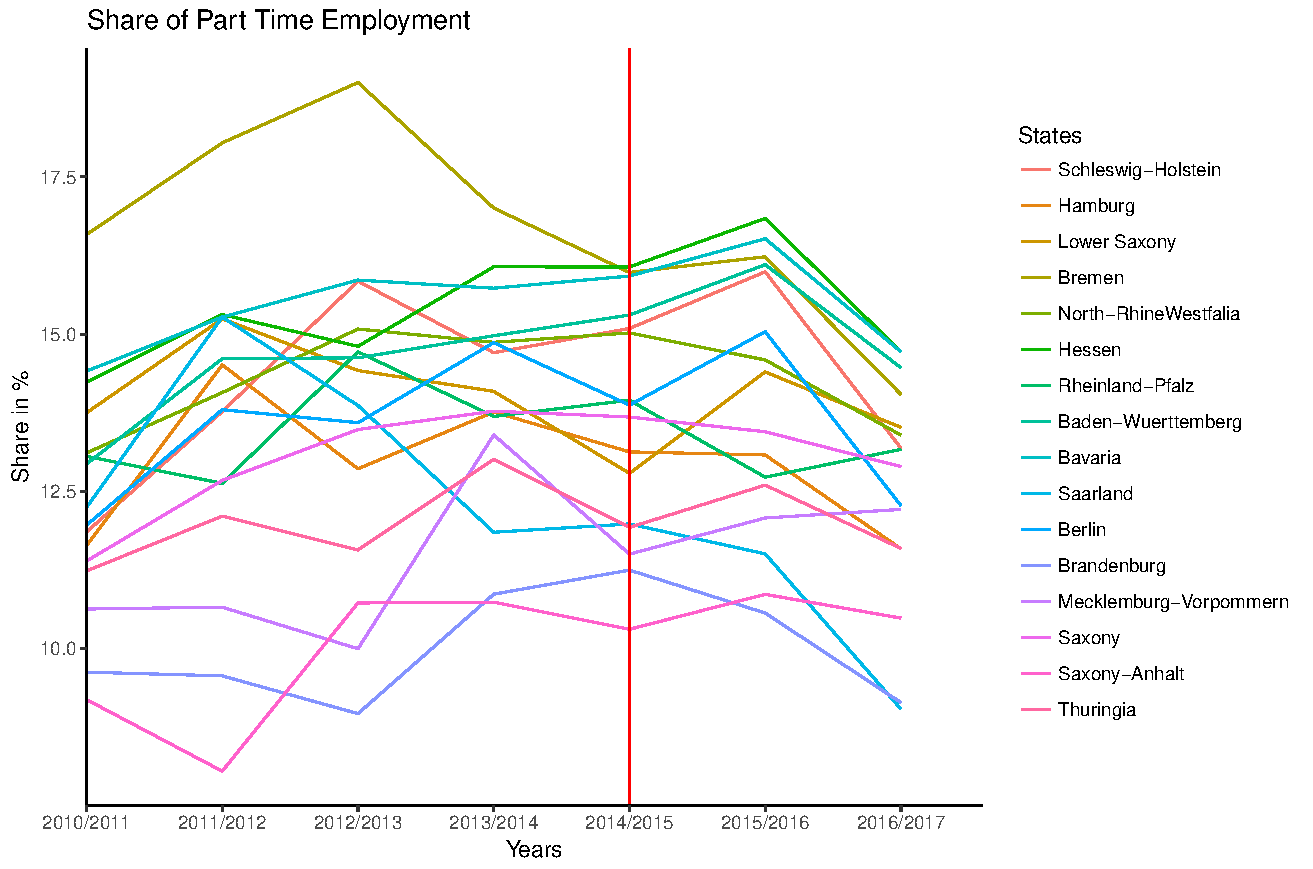
\includegraphics[width=\textwidth]{q4/growthpart.pdf}
\caption{Part time employment}
\end{subfigure}

\begin{subfigure}[h]{0.5\linewidth}
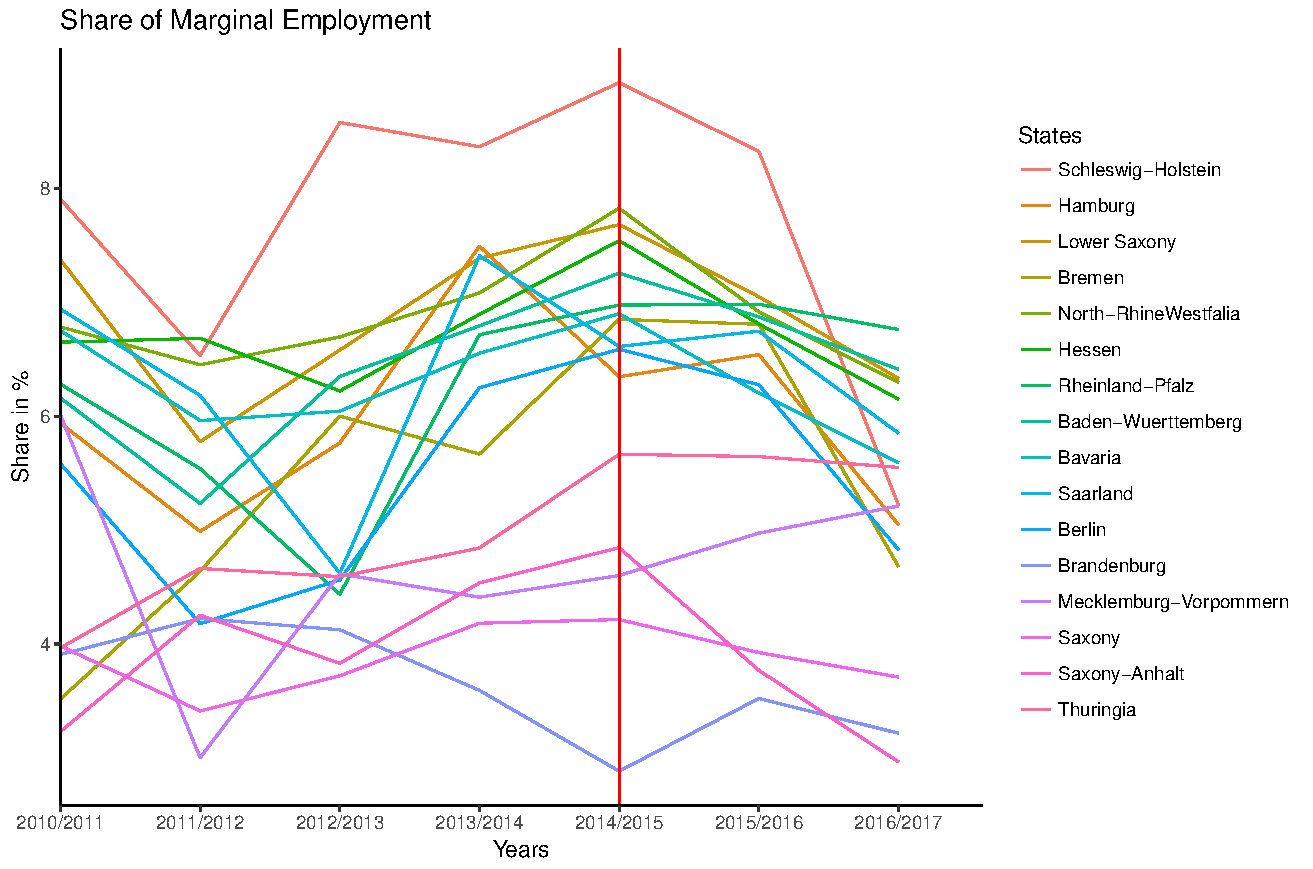
\includegraphics[width=\textwidth]{q4/growthmarginal.pdf}
\caption{Marginal time employment}
\end{subfigure}
\hfill
\begin{subfigure}[h]{0.5\linewidth}
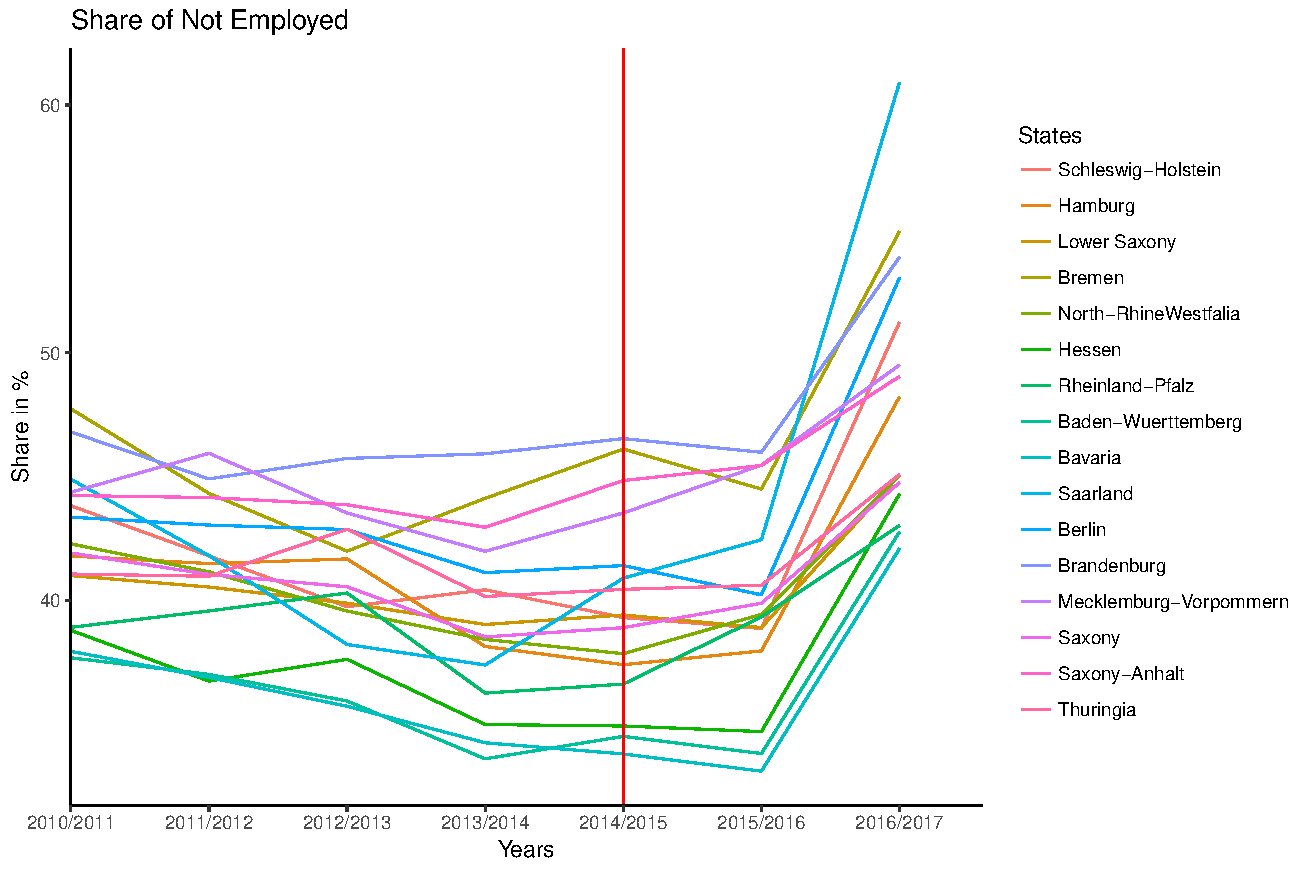
\includegraphics[width=\textwidth]{q4/growthnot.pdf}
\caption{No employment}
\end{subfigure}%
\label{q4graph2}
\end{figure}
%
\newline
Next, we look at the share of employees over time, for each federal state in Germany. As it can be see in figure \ref{q4graph2} we plotted the share of full-time, part-time, marginal and non-employment respectively. These graphs have a similar trend as Figure \ref{q4graph1}, however the trend differs in strength for some states. \newline
Before 2015, the share of full-time employment fluctuated within the states every year around two to five percent, but besides Hamburg and Bremen all other fourteen states had a high growth rate at around 35 to 40 percent.  After the implementation of the minimum wage an overall decrease of around five percentage in the growth rate of full-time employment can be seen. \newline
The share of part-time employment has a similar development and range of differences between the states in the beginning, but not as high. It also does not drop as much, after the implementation of the minimum wage, as the full-time employment. In some states the part-time employment experienced a little increase after the implementation of the minimum wage. Nevertheless the share of part-time employment decreases at around two to three percentage overall, after the implementation of the minimum wage. \newline
The time trend for the share of marginal employment differs. It can be seen, that there are stronger fluctuation before the minimum wage introduction for some states. After the introduction, one can see a decrease, however not for all states. Here, the dynamics do not seem to follow a trend as strong as for the full time or part-time employment. \newline
The share of non-employed people starts out at a high level of around 35 to 48 percentage per year. After the implementation of the minimum wage there is a clearly rise in the growth rate of non-employed of about ten percentage for each state. This is compared to the decreasing share of the different employment groups quit severe. To sum up, these graphs indicate a first trend how the minimum wage affected employment, which is here clearly negative on the employment in Germany. However, there seem to be differences how part-time and marginal employment was affected, as these graphs show the least common trend on state level.
%
%
%
\newpage
\section{Identification Affected Regions}
\subsection{Introduction}
The following section will be used to identify the effected regions by the minimum wage. We follow the strategy of \cite{schmitz2017effects} and \cite{caliendo2017short}, as both use similar approaches.


\subsection{Theory} 
As an indicator, to differentiate between regions affected stronger by the minimum wage and regions which were not affected, one typically has to classify how the minimum wage 'bites' into the regional wage level. Therefore, it is necessary to use two indexes, Kaitz and Fraction. \newline
The Kaitz Index measures the ratio between the nominal legal minimum wage and the average wage, hence it can be calculated by 
\begin{align}
Kaitz_{i,t} = \dfrac{w^{min}}{w_{i,t}^{average}}
\end{align}
for a specific region $i$ in period $t$, with $w^{min} = 8.50${\euro\newline
In contrast, the Fraction Index measures the share of workers affected by minimum wage, thus earn less than 8.50{\euro} per hour. It can be calculated by
\begin{align}
Fraction_{i,t} = \dfrac{E_{i,t}^{min}}{E_{i,t}^{all}}
\end{align}
with $E_{i,t}^{min}$ as the number of workers affected by minimum wage and $E_{i,t}^{all}$ as the number of all workers for a specific region $i$ in period $t$. Both indexes are able to measure the potential affectedness of a region.

\subsection{Implementation}
The basic preprocessing of the data for this quantlet is similar to quantlet 4 and can be seen in chapter 5.3 on page 21. Therefore, it is not going to be repeated in this part. Still, these preprocessing-functions are part of quantlet 5 as well and can be seen in the appendix. \linebreak\linebreak
The data needs to be filtered using the pre-defined \textbf{data\_selector}-function and the labor force has to be adjusted by using the function \textbf{adj\_labor\_force}.
%
As soon as the \textbf{Reduced\_merged}-dataset is available, the processing can begin. Only the people who work are kept in the data. In other words, people with an income above 0 and a working time above 0. Therefore, all other values are set to \textit{NA} by applying the function to the respective dataset.
\begin{lstlisting}
set_working_time_income = function(x) {
	x$Current.Gross.Labor.Income.in.Euro
	[x$Current.Gross.Labor.Income.in.Euro <= 0] = NA
    x$Actual.Work.Time.Per.Week[x$Actual.Work.Time.Per.Week <= 0] = NA
    return(x)
}
Reduced_merged = set_working_time_income(Reduced_merged)
\end{lstlisting}
Again, to drop all observations with missing values, the \textbf{drop\_sub\_na}-function is used, which drops each observation with at least one missing value (source code see chapter 5.3 and appendix). 
%
Next, the function \textbf{create\_hourly\_earnings} is used to compute a new variable \textbf{hourly.earnings}. It is generated using the variable \textbf{Current.Gross.Labor.Income.in.Euro}, which provides the monthly income of one observation, and divided by \textit{4.3} times the \textbf{Actual.Work.Time.Per.Week}. \textit{4.3} was taken, because a months consist approximate of 4.3 weeks and the working time is given in weeks. 
To get more robust and exact values to work with, observations from the first and last percentile of hourly earnings are dropped. Once again, the the new function is applied to the data set. 
\begin{lstlisting}
create_hourly_earnings = function(x) {
	x$Hourly.earnings = x$Current.Gross.Labor.Income.in.Euro/(4.3 * \\
	x$Actual.Work.Time.Per.Week)
	x$Hourly.earnings[x$Hourly.earnings> \\
    	quantile((x$Hourly.earnings),c(0.99))|
	x$Hourly.earnings < \\ 
    	quantile((x$Hourly.earnings), c(0.01))] = NA
	x = x[complete.cases(x$Hourly.earnings), ]
    return(x)
}
Reduced_merged_noNA = create_hourly_earnings(Reduced_merged_noNA)
\end{lstlisting}
%
Now, a dummy for observations affected by the minimum wage is generated. The variable has the value \textit{one} if the hourly earnings are smaller than 8.50 and \textit{zero} otherwise. To make it reusable another function is used, called \textbf{dummy\_minimum\_wage}. Afterwards, the function is applied to the data set \textbf{Reduced\_merged} and assigned the same variable.
\begin{lstlisting}
dummy_minimum_wage = function(x) {
    x$Subject.to.minwage = NA
    x$Subject.to.minwage[x$Hourly.earnings < 8.5] = 1
    x$Subject.to.minwage[is.na(x$Subject.to.minwage)] = 0
    return(x)
}
Reduced_merged_noNA = dummy_minimum_wage(Reduced_merged_noNA)
\end{lstlisting}
For the upcoming analysis it is important to see how certain variables develop over time and state. Thus a function to collapse the dataset is generated and applied to the data set as usually. In detail, the dataset is grouped by the variables \textbf{State.of.Residence} and \textbf{Wave}, which means that all observation for a specific state in a specific year are grouped together. The new dataset is called \textbf{dbys} (data by year and state).
\begin{lstlisting}
collapse_dataset = function(x) {
    x %>% group_by(State.of.Residence, Wave) %>% summarise(n(), 
    Hourly_earnings = mean(Hourly.earnings, na.rm = TRUE), 
    AvgInc = mean(Current.Gross.Labor.Income.in.Euro, na.rm = TRUE),
    Avg.Weekly.Working.Time = mean(Actual.Work.Time.Per.Week, 
        na.rm = TRUE), Fraction = mean(Subject.to.minwage))
}
dbys = collapse_dataset(Reduced_merged_noNA)
\end{lstlisting}

As a next step, the function \textbf{generate\_index} is used to generate both Kaitz and Fraction-Index. At the beginning, the change of Fraction-Index over time and state is created. The same was done for the Kaitz-Index afterwards. As a last step, the generated function is applied to the\textbf{dbys} data set. 
\begin{lstlisting}
generate_index = function(x) {
    x$Delta.Fraction = c(0, diff(x$Fraction))
    x$Kaitz = 8.5/x$Hourly_earnings
    x$Delta.Kaitz = c(0, diff(x$Kaitz))
    return(x)
}
dbys = generate_index(dbys)
\end{lstlisting}

The creation of a correlation variable of both Bites is needed for later  graphical analysis and generated as followed.  
\begin{lstlisting}
generate_correlation = function(x) {
    x %>% group_by(Wave) %>% 
    summarise(Correlation.Fraction.Kaitz = 
    cor(Fraction, Kaitz, use = "all.obs", 
    method = "pearson"))
}
Correlation.Bites.yearly = generate_correlation(dbys)
\end{lstlisting}

Again, the use of the function \textbf{create\_periods} is necessary. The source code of this function can be seen in chapter 5.3 as well as in the appendix.
\begin{lstlisting}
Correlation.Bites.yearly$Period = create_periods(list_years)
\end{lstlisting}

Here, a function to summarize the correlation between Fraction and Kaitz is created. This function is later on used to generate further graphs, showing the correlation of the bites over time and state. 
\begin{lstlisting}
summarize_corr_fk = function(x) {
    x %>% group_by(State.of.Residence) %>% 
    summarise(Correlation.Fraction.Kaitz = cor(Fraction, Kaitz, 
    use = "all.obs", method = "pearson"))
}
Correlation.Bites.State = summarize_corr_fk(dbys)
\end{lstlisting}

The Shapiro Test is conducted by a function, containing a loop and then applied to the dataset \textbf{dbys} using \textbf{shapiro\_test} and the \textbf{list of years} to test whether the two Bites are normally distributed over time and state. 

Except for 2010, these statistical significance tests confirm the normally distribution for the Kaitz Index at a significance level of five percent. For the Fraction Index it confirms the normally distribution for all years at a significance level of five percent. 
\begin{lstlisting}
shapiro_test = function(input, mode, list_years) {
    if (mode == "Fraction") {
        input$mode = input$Fraction
    } else if (mode == "Kaitz") {
        input$mode = input$Kaitz
    } else {
        print("Mode must be either Fraction or Kaitz!")
    }
    for (years in 1:length(list_years)) {
        test = shapiro.test(input$mode[input$Wave == list_years[years]])       			print(list_years[years])
        print(test)
    }
}
shapiro_test(dbys, "Kaitz", list_years)
shapiro_test(dbys, "Fraction", list_years)
\end{lstlisting}

\subsection{Output}
The following output section consist out of three different groups of graphs each for the Fraction and the Kaitz-Index. We focus on the development of both Bites over time, the density of the Bites over time and the correlation between both Bites over states and time.
%
\begin{figure}
\caption{Fraction and Kaitz Index over Time}
\begin{subfigure}[h]{0.5\linewidth}
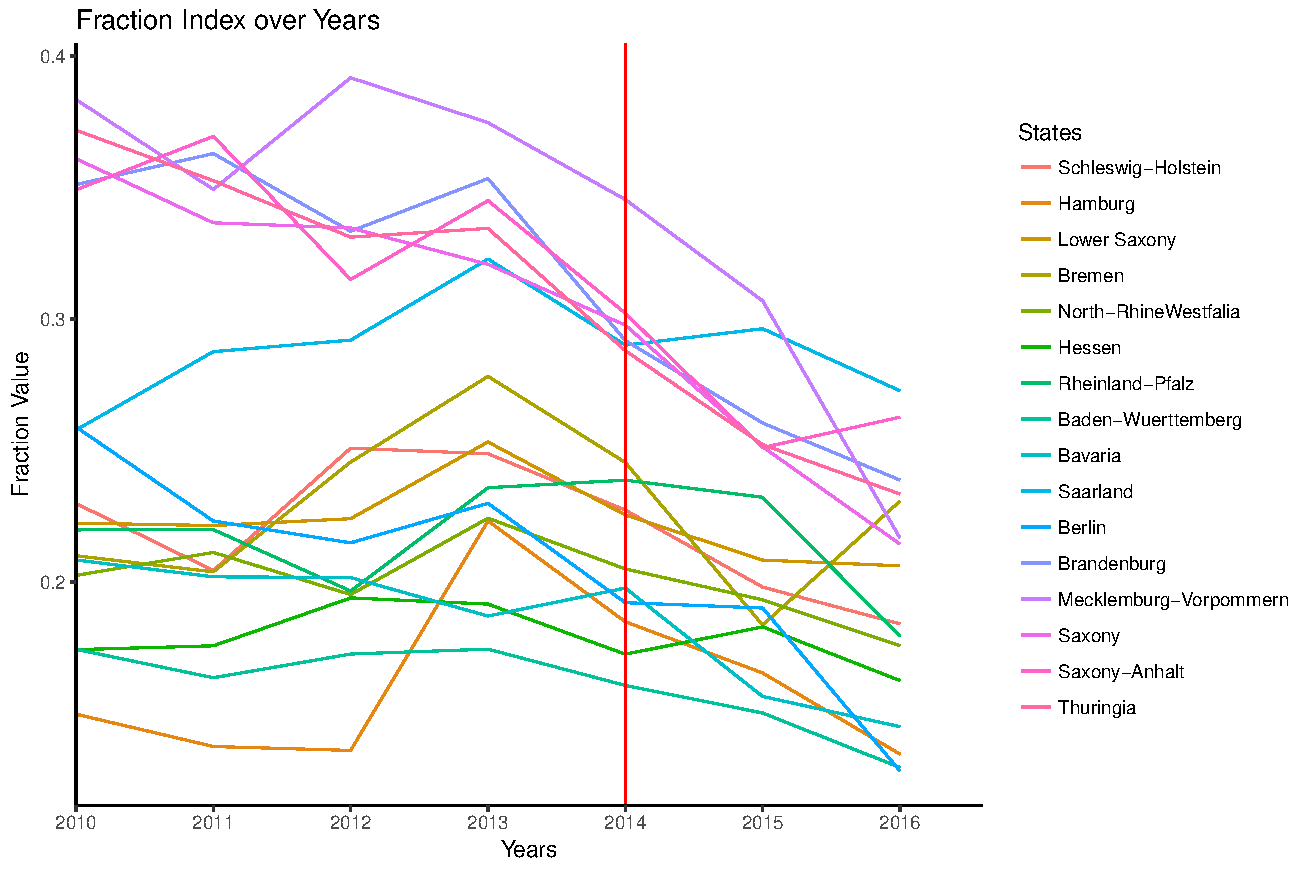
\includegraphics[width=\textwidth]{q5/aggregateddatafraction.pdf}
\caption{Fraction Index}
\end{subfigure}
%
\begin{subfigure}[h]{0.5\linewidth}
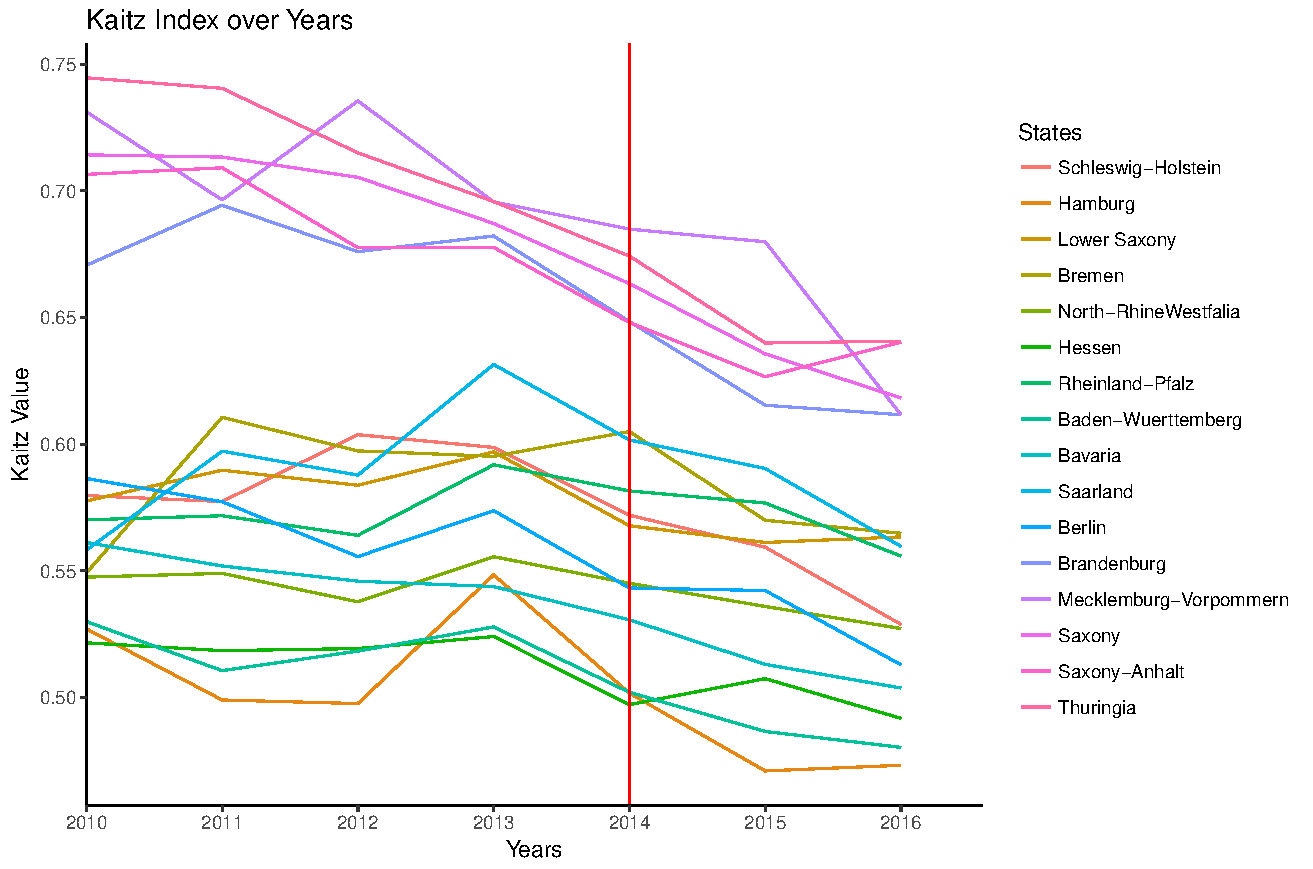
\includegraphics[width=\textwidth]{q5/aggregateddatakaitz.pdf}
\caption{Kaitz Index}
\end{subfigure}
\label{q5graph1}
\end{figure}
%
%
%
Figure \ref{q5graph1} displays the development of both, Fraction (a) and Kaitz Index (b), for each state in Germany from the years 2010 until 2016. The trend of the Fraction Index, depending on the state, evolves quite different and is not very identifiable before the minimum wage introduction. However, after the introduction, the Fraction Index falls for all states. %
The Kaitz Index graph indicates a downward sloping trend. Both graphs imply, that the minimum wage changed the wage levels of each state in Germany.


\begin{figure}
\begin{subfigure}[h]{0.5\linewidth}
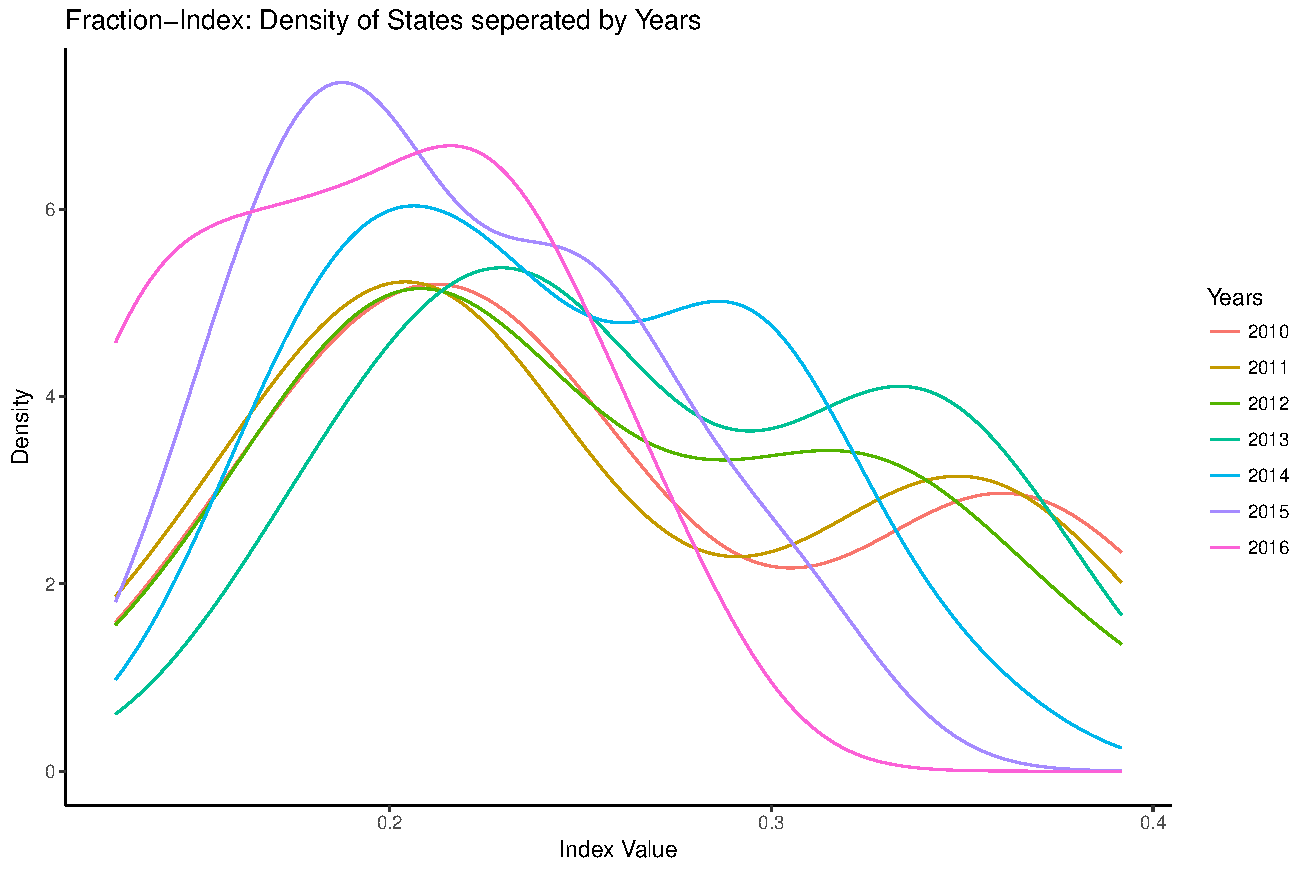
\includegraphics[width=\textwidth]{q5/densityaggrfraction.pdf}
\caption{Density Fraction Index}
\end{subfigure}
\hfill
\begin{subfigure}[h]{0.5\linewidth}
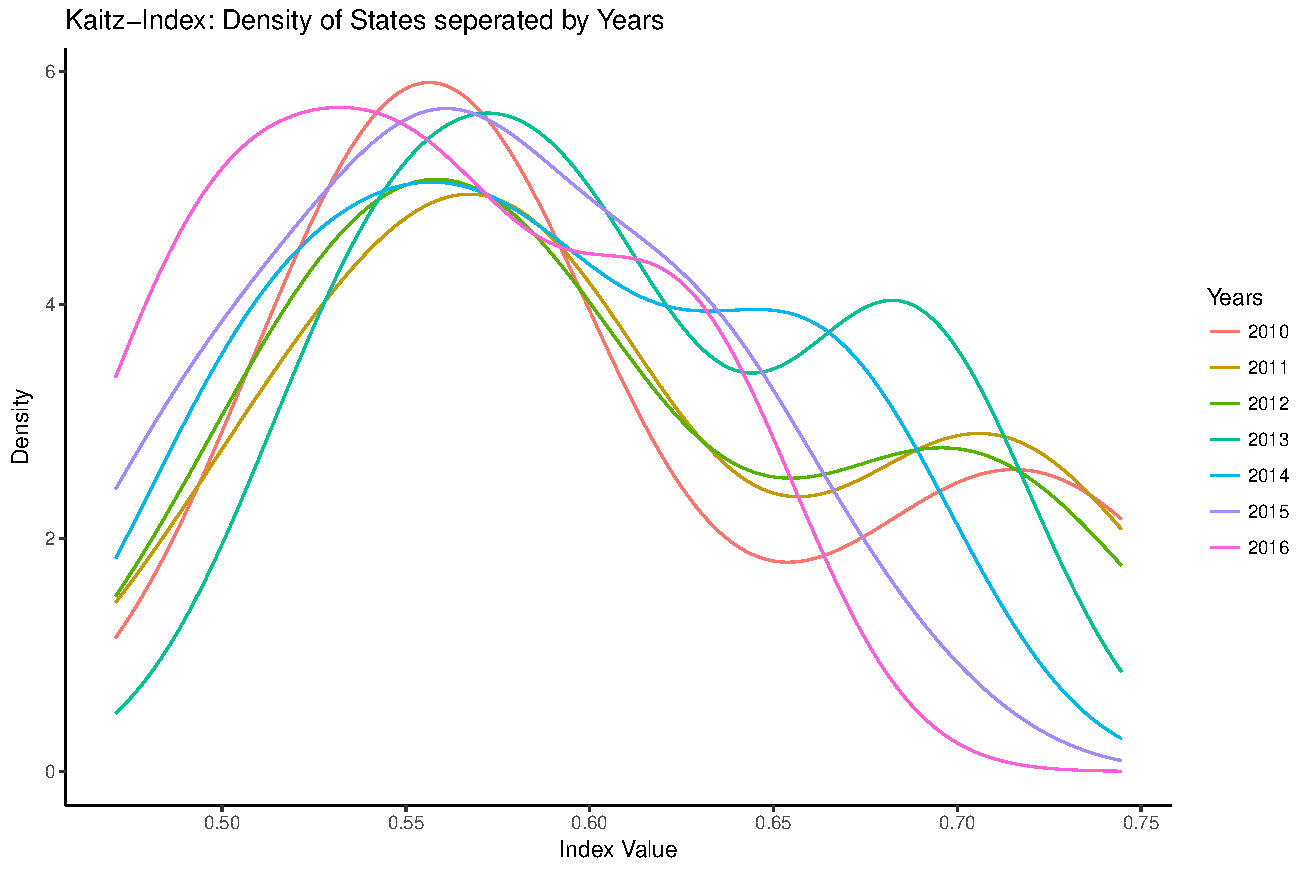
\includegraphics[width=\textwidth]{q5/densityaggrkaitz.pdf}
\caption{Density Kaitz Index}
\end{subfigure}%
\caption{Density Plots for Fraction and Kaitz-Index}
\label{q5density}
\end{figure}
The density plots in figure \ref{q5density} give information about the characteristics and skewness of the data. The density of the Fraction Index is right skewed with an additional higher density at the end. This can be seen in a similar form for each year. It shows a high density at around the index of 0.2 and an other peak at around 0.35. This second peak gets flattened after the implementation of the minimum wage. The graph for the Kaitz Index shows a similar density as the one of the Fraction. The only difference is that it is a little smoother over the years. The peaks of the graph are at 0.55 and 0.7, with the second peak shifted far to the left and almost eliminated after the implementation of the minimum wage.  

\begin{figure}[h]
\caption{Correlation Bites over States}
\centering
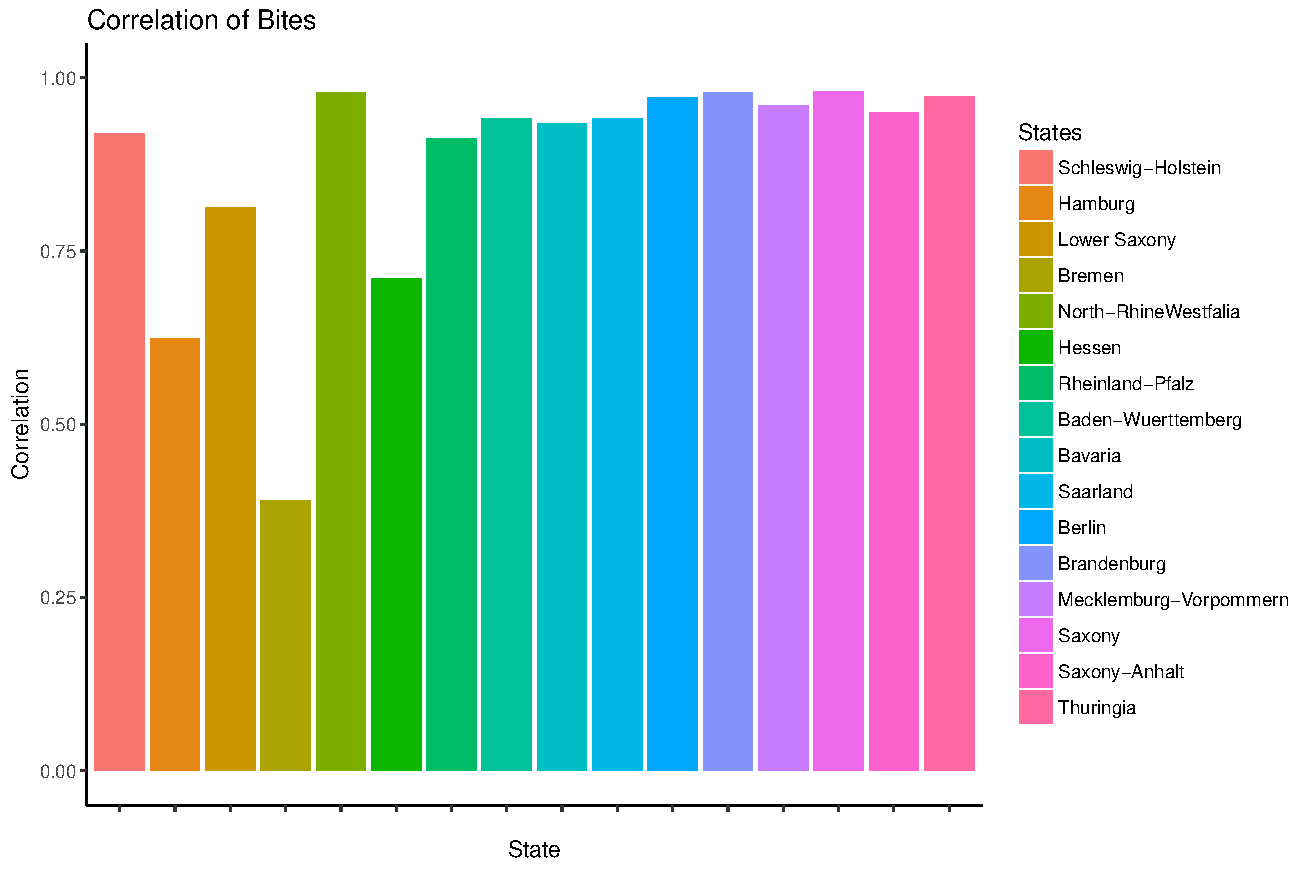
\includegraphics[width=0.75\textwidth]{q5/outputcorrelationbitesstates.pdf}
\label{q5cor1}
\end{figure}
Figure \ref{q5cor1} displays the correlation of Fraction Kaitz Index over the years for each state. The result, is quite interesting, as there seem to be states in which the bites are less correlated over the years, especially in Bremen. This implicates, that the wage structure in Bremen differs a lot. Also for other states, such as Hamburg, Hessen or Lower Saxony the correlation is not as strong as in the remaining states. \newline
\begin{figure}[h]
\caption{Correlation Bites over Years}
\centering
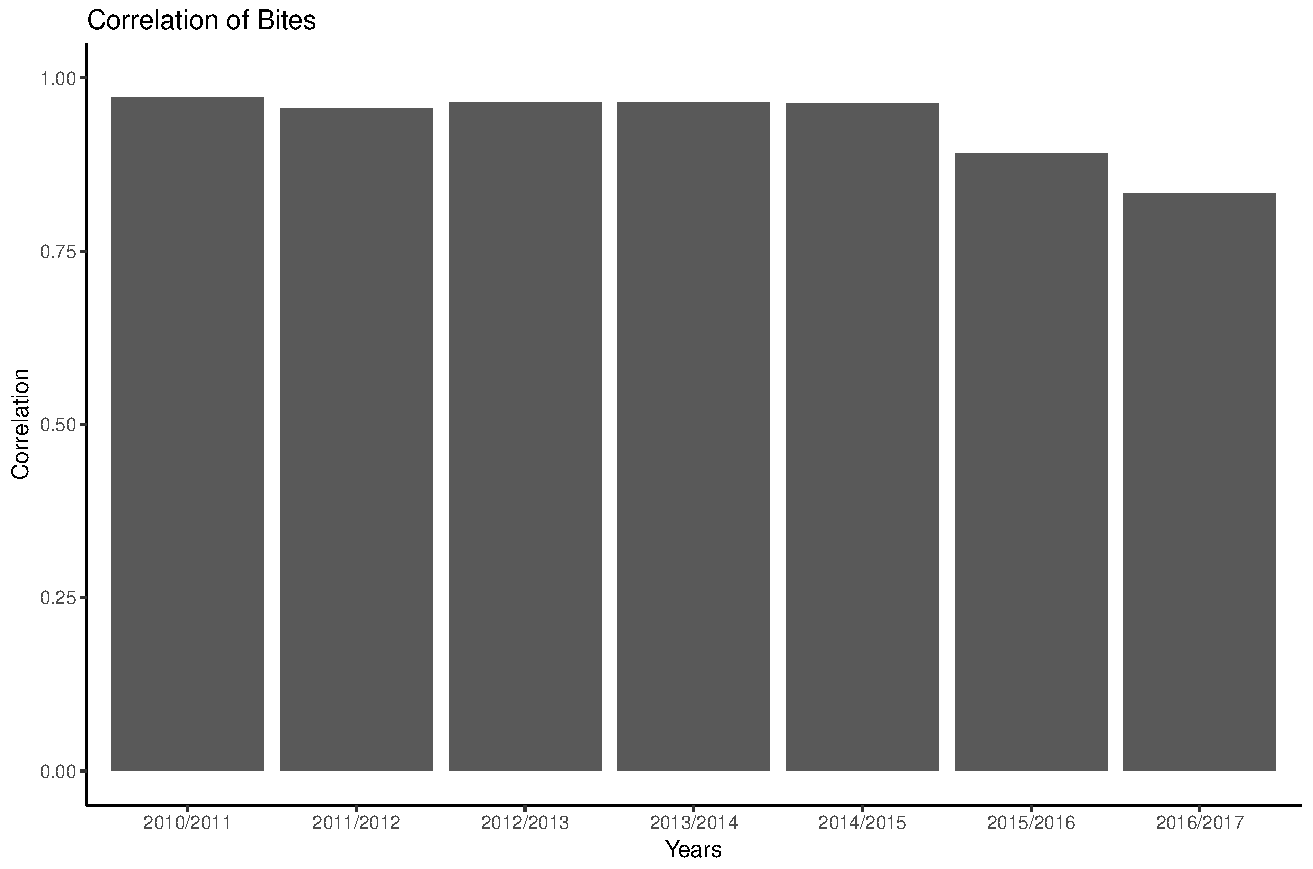
\includegraphics[width=0.75\textwidth]{q5/outputcorrelationbitesyearly.pdf}
\label{q5cor2}
\end{figure}
Figure \ref{q5cor2} displays the correlation of the Indexes for each year. The correlation was stronger before the implementation of the minimum wage. This implies, that the Indexes are affected differently as the correlation sinks, after the implementation.
%
\newpage
\section{Graphical Analysis of Minimum Wage Effect}
\subsection{Introduction}
In this section it is about the graphically analysis how the minimum wage "bites" into the different German states. Thus, it is important to compare the Kaitz and Fraction Indexes for each state over time. This issue is addressed in this Section and visualize the change of Kaitz and Fraction Index over time. In order to visualize Indexes not over time but rather in a geographical context we make use of another data frame from GADM. GADM provides maps and spatial data on administrative boundaries, thus it is ideal to visualize a map of Germany on federal state level given the input data, here Fraction and Kaitz Index. Furthermore, the data is freely available for academic use.

\subsection{Theory}
In addition to the continuous treatment assignment by the state and time specific bite values, it is also possible to generate a binary treatment. Thus, similar to \cite{schmitz2017effects}, it is generated two binary treatment dummy variables. The binary treatment assignment is made with the aid of the Kaitz Index from 2013. More specific, for the standart binary treatment it is usefull to divide the states by the median of the Kaitz Index from 2013. All states with an Index higher than the median will be assigned the value \textit{one}. Consequently, the states with an Index below the median will be assigned the value \textit{zero}. For the robust binary treatment, the assignment is done by a slightly different approach. Instead, of using the median as the indicator whether a state is in the treatment or control group, it is used the 60\% - percentil and 40\% - percentil respectively. Thus, this method leaves out the states within these two percentiles and makes the binary treatment assignment more robust.

\subsection{Implementation}
In order to run the following code, it is necessary to pre-run the Quantlets 1, 4 and 5 as this section needs the aggregated datasets \textbf{Employment.yearly} and \textbf{dbys}. In a first step, a merge of these two datasets is necessary, which is done with the following function in a general way.
\begin{lstlisting}
combine_data = function(x, y) {
    combined = merge(x, y)
    combined = combined %>% group_by(Wave, State.of.Residence) %>% 
    	arrange(Wave)
    return(combined)
}
\end{lstlisting}
The function \textbf{combine\_data} merges two data frames \textit{x} and \textit{y} using the merging variables \textbf{Wave} and \textbf{State.of.Residence} and arranging the newly combined data frame by the variable \textbf{Wave}.

As already mentioned, this function is to combine the data frames \textbf{Employment.yearly} and \textbf{dbys}, naming the newly merged data frame \textbf{analyze\_tc}, which will be the main data frame from now on.
\begin{lstlisting}
analyze_tc = combine_data(Employment.yearly.state, dbys)
\end{lstlisting}
Through merging the previous two data frames together, now there is a data frame which combines both, employment variables and the Index variables for each state in each year. \newline
Next, it is generated the two previously mentioned binary treatment variables. This again is done by using a function, called \textbf{data\_selector}.
\begin{lstlisting}
data_selector = function(analyze_tc, wave) {
    select(filter(analyze_tc, Wave == wave), c(Wave,
    	State.of.Residence, Kaitz, Fraction))
}
\end{lstlisting}
The main feature of this function is the \textbf{select} command, which is a feature of the \textbf{dplyr}-package. In particular, this makes it possible to draw a subset of a given data frame. As it is need to use the Kaitz and Fraction Indexes of the year 2013 for the binary treatment assignment, this function are used to generate a subset with the variables \textbf{Wave}, \textbf{State.of.Residence}, \textbf{Kaitz} and \textbf{Fraction} from the previous generated data frame \textbf{analyze\_tc} using the year 2013 as a filter.
\begin{lstlisting}
# Create subset for 2013
analyze_2013 = data_selector(analyze_tc, 2013)
\end{lstlisting}
Note, that it is possible to draw a subset for each year individually, when changing the value in the function accordingly. \newline
Subsequently, the binary treatment variables are generated in the filtered data frame \textbf{analyze\_2013}. This is done by a function called \textbf{add\_treatment}.

\begin{lstlisting}
add_treatment = function(x) {
    x$binary_treatment1 = NA
    x$binary_treatment1[x$Kaitz > median(x$Kaitz)] = 1
    x$binary_treatment1[is.na(x$binary_treatment1)] = 0
    x$binary_treatment2 = NA
    x$binary_treatment2[x$Kaitz > quantile(x$Kaitz, c(0.6))] = 1
    x$binary_treatment2[x$Kaitz < quantile(x$Kaitz, c(0.4))] = 0
    return(x)
}
\end{lstlisting}
This function generates the treatment variables \textbf{binary\_treatment1} and \textbf{binary\_treatment2} corresponding to the mentioned theory in Section 7.2 for a given data frame \textit{x}.
In detail, a new variable \textbf{binary\_treatment1} is generated with missing values. Next, this variable will be assigned the value 1 if the Kaitz Index of the observation is bigger than the median of the Kaitz Index. Correspondingly, the value 0 is assigned to all other variables which are still set as NA. Likewise is the generation of the variable \textbf{binary\_treatment2}, which is supposed to indicate the robust treatment assignment. As mentioned above, the assignment is done with the 60\% - and 40\% quantile. Therefore, the \textbf{quantile} command in the \textbf{add\_treatment} function is used. 

The function is applied to the dataframe \textbf{analyze\_2013}. 
\begin{lstlisting}
# Apply add_treatment with analyze_2013 dataset
analyze_2013 = add_treatment(analyze_2013)
\end{lstlisting}
In a last step, the treatment variables are merged back into the main dataframe \textbf{analyze\_tc}.
\begin{lstlisting}
# Set Treatment Identifiers to the same column in the main data
analyze_tc$binary_treatment1 = analyze_2013$binary_treatment1
analyze_tc$binary_treatment2 = analyze_2013$binary_treatment2
\end{lstlisting}
As \textbf{analyze\_tc} is ordered by Wave and State of Residence and \textbf{analyze\_2013} is ordered by State of Residence as well, this allows for the simple add of the treatment variables, without further specifications. \newline
Thus, the data frame \textbf{analyze\_tc} has all needed variables for the graphical representation. In order to analyze the binary treatment the data has to be grouped by the treatment variable values respectively. This is done with the \textbf{group\_by} command. We apply a function called \textbf{aggregate\_treatment\_control} with two input values.
\begin{lstlisting}
aggregate_treatment_control = function(x, y) {
    if (y == 1) {
        x$y = x$binary_treatment1
    } else if (y == 2) {
        x$y = x$binary_treatment2
    }
     x = x %>% group_by(Wave, y) %>% summarise(Observation = n(),
       Avg.Log.Full.Employment = mean(Log.Full.Employment,
          na.rm = TRUE),  
       Avg.Delta.Log.Full.Employment = 									mean(Delta.Log.Full.Employment, na.rm = TRUE), 				          Avg.Full.Employment.Rate = mean(Full.Employment.Rate, 
          na.rm = TRUE),
    if (y == 1) {
        x$binary_treatment1 = x$y
    } else if (y == 2) {
        x$binary_treatment2 = x$y
    } else {
        print("Only 1 and 2 are valid as values for y!")
    }
    x$y = NULL
    return(x)
}
\end{lstlisting}
As one can see, the input value \textit{x} is the data frame, from which the data will be used. The value \textit{y} can only take the values one or two. If for instance, $ y = 1 $, the function will group the data by \textbf{Wave} and \textbf{binary\_treatment1}. The variables in the new aggregated data frame are all means of the grouped variables.

Two aggregated dataframes are generated with the function \textbf{aggregate\_treatment\_control}, one for each binary treatment, called \textbf{Treatment.analysis1} and \textbf{Treatment.analysis2}.
\begin{lstlisting}
Treatment.analysis1 = aggregate_treatment_control(analyze_tc, 1)
Treatment.analysis2 = aggregate_treatment_control(analyze_tc, 2)
\end{lstlisting}

As the data frame \textbf{Treatment.analysis2}, is created by grouping by \textbf{Wave} and \textbf{binary\_-treamtment2}, it contains observations with missing values, as no values are defined for the variable \textbf{binary\_-treamtment2} for all observations. Thus these observations are dropped with applying the \textbf{drop\_sub\_na} function.
\begin{lstlisting}
# Apply drop_sub_na to Treatment.analysis2 to drop lines with missing values
Treatment.analysis2_noNA = drop_sub_na(Treatment.analysis2)
\end{lstlisting}
For the map visualization the data first are loaded into R. The datacontent is stored in \textit{.rds} format, which stands for 'R SpatialPolygonsDataFrame'. These datafiles can easily be loaded into R with the \textbf{readRDS} command.
\begin{lstlisting}
map = readRDS("SOEPQ6_GraphicalAnalysisMinWage/geodata/DEU_adm1.rds")
\end{lstlisting}
The individual German federal states are represented as factors in the SOEP data set. The name of the federal state is assigned as a label, indicating the English name. This is in conflict with the previously loaded map data set, which contains the German federal states in the German language. The \textbf{substituteState} function is therefore used to define the factor levels as numeric and replace them with the German identifier. The function receives the column \textit{State.of.Residence} of the data set of the respective year as input. This step must be taken because the alphabetical sorting in English and German leads to a differing order. The \textbf{correctState} function then replaces the column completely with cleaned designators by sorting the data frame alphabetically according to the State.of.Residence column. The column \textit{State.of.Residence} will then be replaced by a vector containing adjusted names of the federal states in German. Furthermore, the \textit{binary.treatment1} variable is converted into a factor variable in this function. This is not directly related to the state conversion, but this step must generally be taken to prepare the data appropriately.

\begin{lstlisting}
# Correct and Order the State Names, so that the names are distinct
correctState = function(x) {
    # Order it alphabetically, ascending
    x = x[order(x$State.of.Residence), ]
    # Define the Treatment as Factor
    x$binary_treatment1 = as.factor(x$binary_treatment1)
    # List with all State Names
    x$State.of.Residence = c([FULL STATE LIST SEE APPENDIX])
    return(x)
}
# Apply the correctState to the analyze_2013 dataset
analyze_2013 = correctState(analyze_2013)
\end{lstlisting}
To generate the final map data, the \textbf{createMapdata} function is created in the following part. 
The analysis data must be merged with the map data and thus brought into a conforming format, which can be processed by \textbf{ggplot2}. For this purpose, the data frame \textit{data\_combined} is created, which contains following columns:
\begin{itemize}
\item id 
\begin{itemize}
\item rownames of the map input data, which range from 1-16 and represent the 16 German states
\end{itemize}
\item State.of.Residence 
\begin{itemize}
\item names of the German federal states according to the map input data
\end{itemize}
\end{itemize}

Afterwards, this data frame is merged with the input data (in this case: analyze\_2013) via a left join. Using the \textbf{fortify}-function, the input map data gets fitted to a linear model and stored as \textit{map2}, which can be proceeded by \textbf{ggplot2}. Lastly, the \textit{map2} gets left joined to the formerly created \textit{data\_combined} by the \textit{id}-column.
The newly created \textbf{createMapdata} function is applied to the prepared SOEP data set and the imported Germany Map.

\begin{lstlisting}
createMapdata = function(input_map, input) {
    data_combined = data_frame(id = rownames(input_map@data), 
    State.of.Residence = input_map@data$NAME_1) %>%
        left_join(input, by = "State.of.Residence")
    map2 = fortify(input_map)
    final_map = left_join(map2, data_combined, by = "id")
}
final_map = createMapdata(map, analyze_2013)
\end{lstlisting}

Based on the \textbf{final\_map} generated by \textbf{createMapdata} the plots are now created. Two additional functions are defined for this in order to be able to record different input data. The first plot function \textbf{plot\_result\_factor} creates a plot based on the binary groups (\textbf{variable binary\_treatment}) and takes as input data only a compliant data set like \textbf{final\_map}. The \textbf{plot\_result\_index} function is configured to generate a plot for the \textit{Fraction}- or \textit{Kaitz}-index. In addition to the input data, this function also acquires information about the variable to be processed and a color channel. The input value \textit{mode} must be either \textit{Fraction} or \textit{Kaitz}, the value \textit{highcolor} must correspond to the \textit{ggplot}-compatible colors. Otherwise, an error will be thrown. Based on the \textit{mode} input value, an if condition is used to decide whether \textit{Fraction} or \textit{Kaitz} is selected. Afterwards, the respective variables are declared. 
These functions can be found in the complete program code in the appendix. The mode value is used once more to create the plot title, which is generated via the \textbf{paste} function.

\begin{lstlisting}
plot_result_index = function(input, mode, highcolor) {
    if (mode == "Fraction") {
        input$mode = input$Fraction
    } else if (mode == "Kaitz") {
        input$mode = input$Kaitz
    } else {
        print("Mode must be Fraction or Kaitz!")
    }
    ggplot(input, aes(x = long, y = lat, group = group)) + 
    	geom_polygon(data = input, aes(fill = mode),
    [REMAINING PART SEE APPENDIX]
    	labs(title = paste(mode, "Index", sep = "-"))
    [REMAINING PART SEE APPENDIX]
}
\end{lstlisting}

Once the functions have been defined, they can be applied by specifying the respective input data and parameters. The results are maps of Germany whose areas (federal states) are colored according to the desired output using a color scale or a binary color scheme.
\begin{lstlisting}
plot_result_factor(final_map)
plot_result_index(final_map, "Fraction", "red")
plot_result_index(final_map, "Kaitz", "blue")
\end{lstlisting}

\subsection{Output}
After grouping the states for both, the standard and robust treatment assignment, it is rather easy to plot the the log employment levels of treatment and control groups using \textbf{ggplot}. Hence, this section will briefly discuss the the graphs and map visualization.


\begin{figure}
\begin{subfigure}[h]{0.5\linewidth}
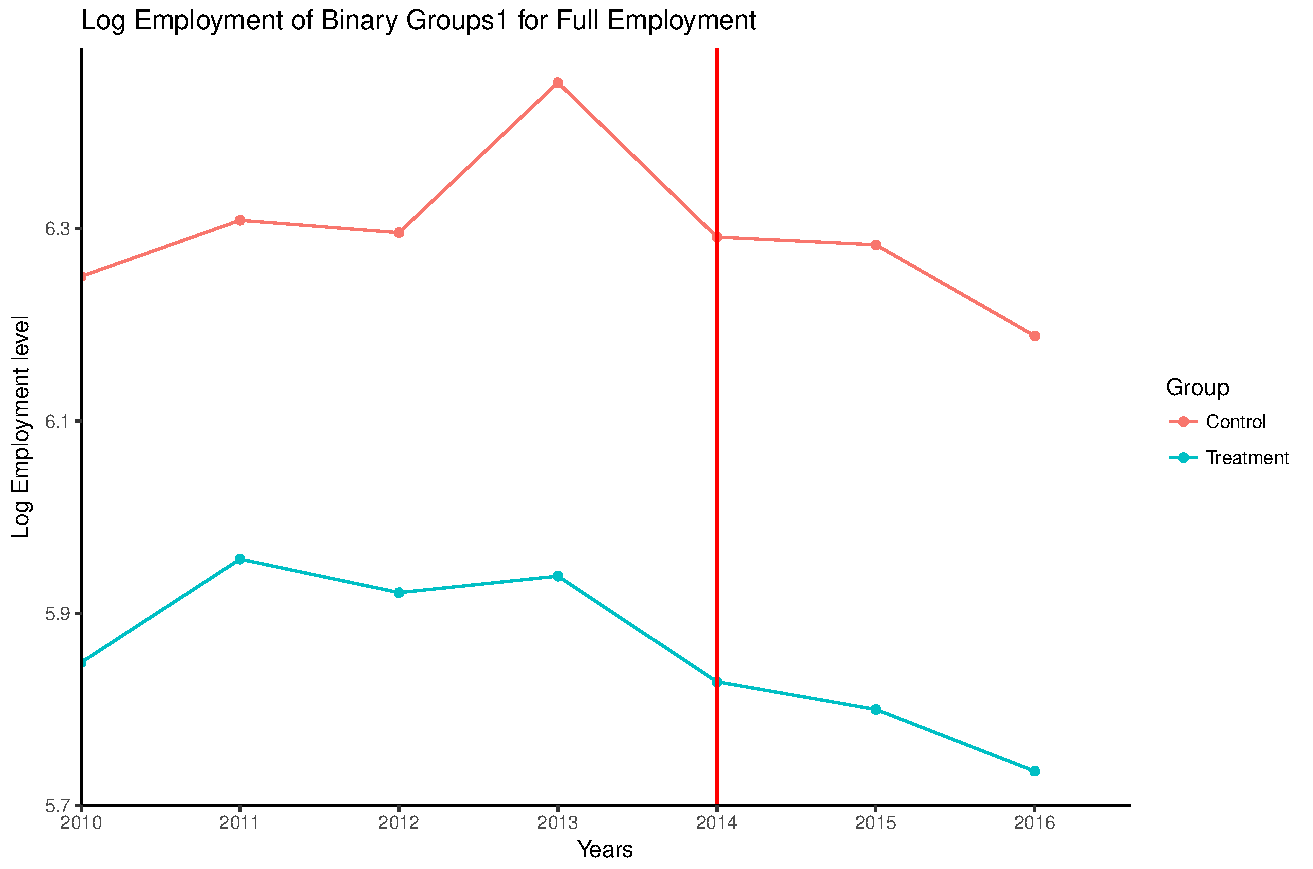
\includegraphics[width=\textwidth]{q6/plot_treatment_t1full.pdf}
\caption{Standard Treatment}
\end{subfigure}
\hfill
\begin{subfigure}[h]{0.5\linewidth}
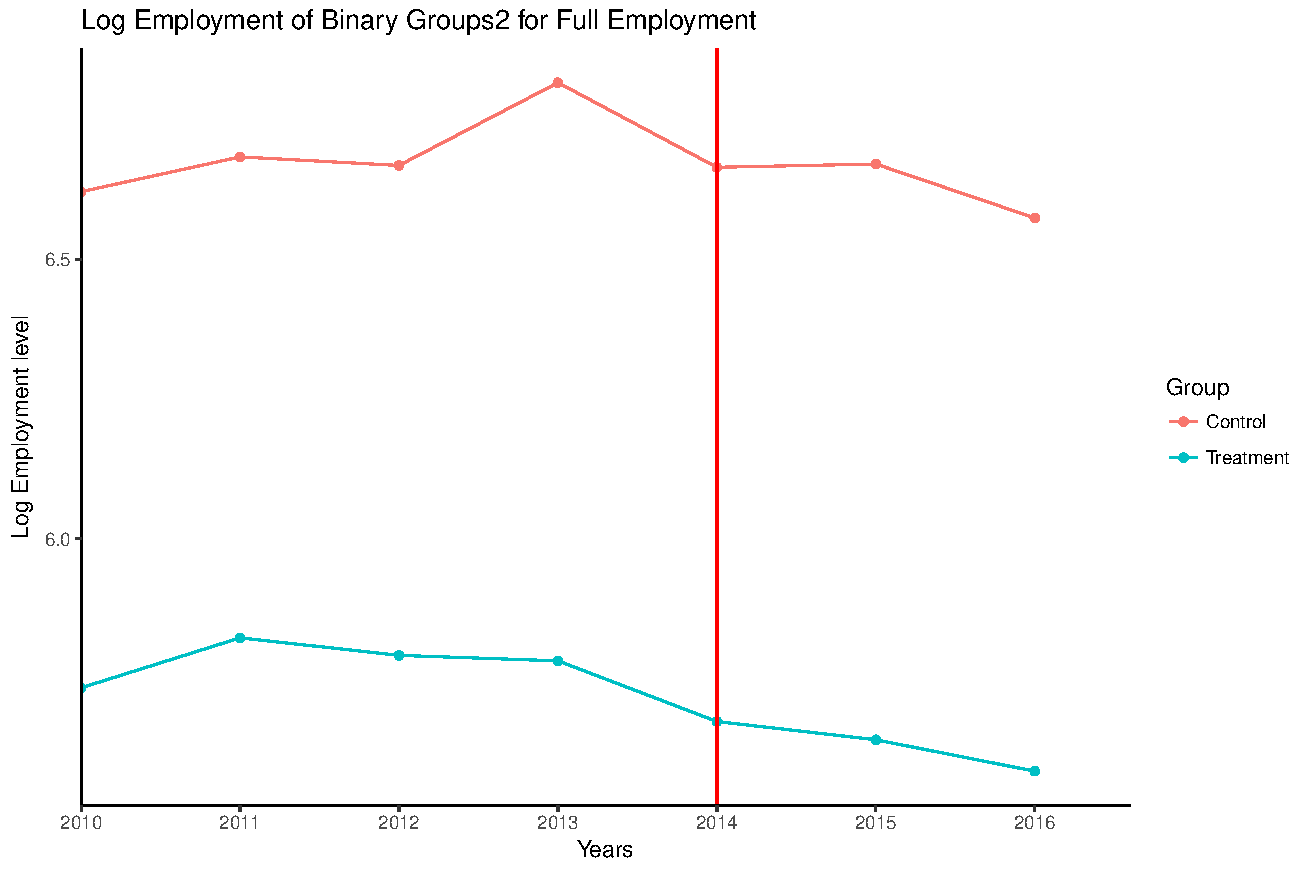
\includegraphics[width=\linewidth]{q6/plot_treatment_ta2full.pdf}
\caption{Robust Treatment}
\end{subfigure}%
\caption{Log Full Time Employment}
\label{q6f}
\end{figure}

\begin{figure}
\begin{subfigure}[h]{0.5\linewidth}
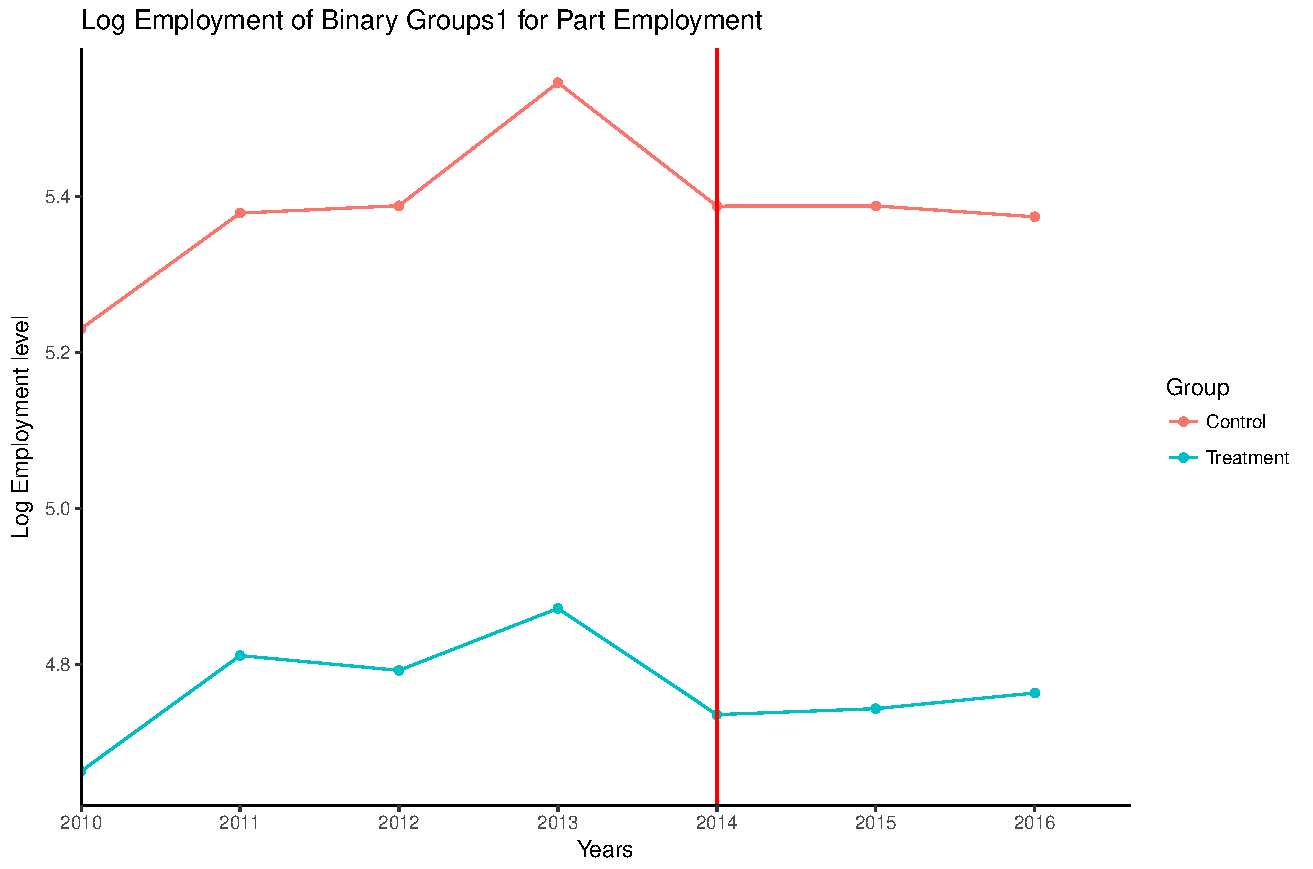
\includegraphics[width=\textwidth]{q6/plot_treatment_t1part.pdf}
\caption{Standard Treatment}
\end{subfigure}
\hfill
\begin{subfigure}[h]{0.5\linewidth}
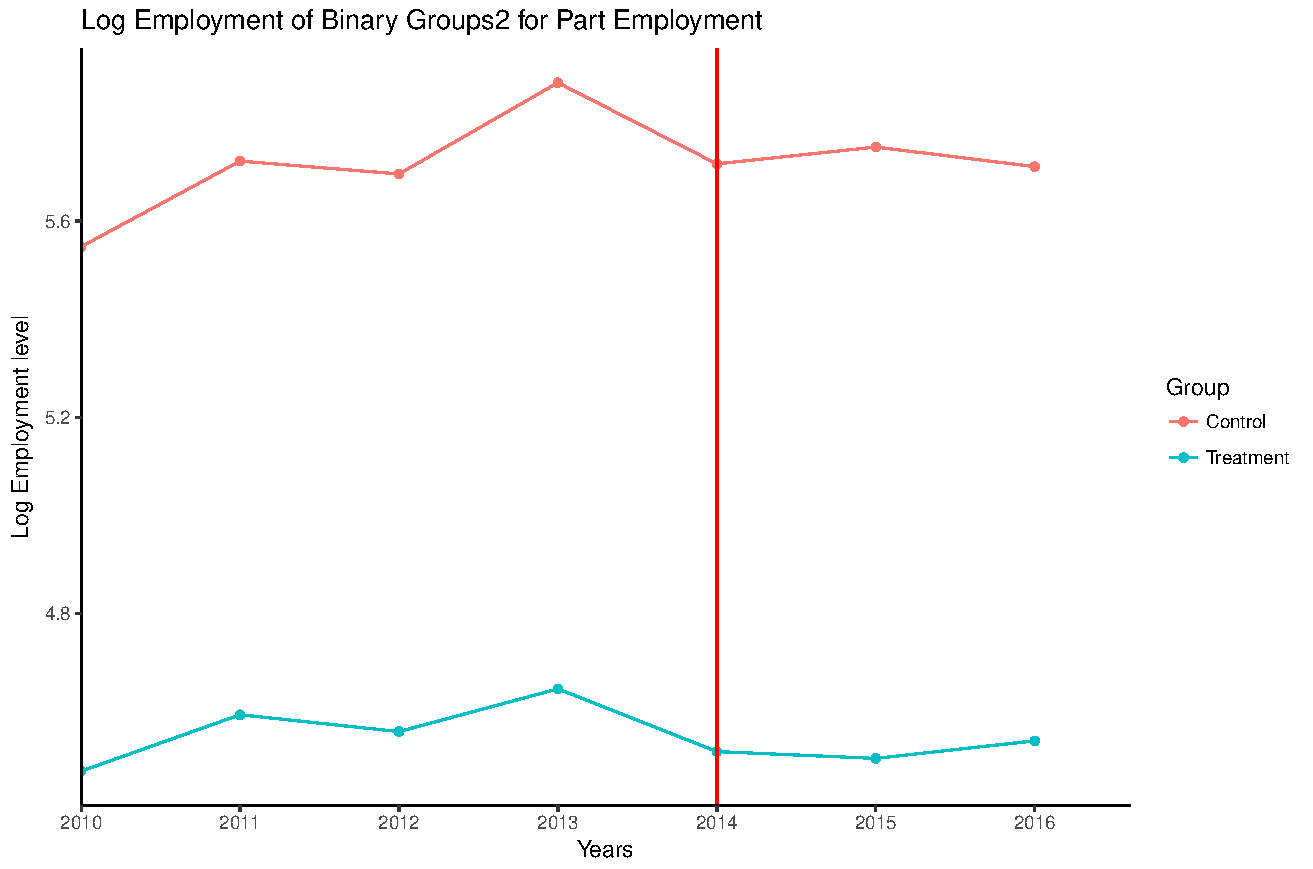
\includegraphics[width=\textwidth]{q6/plot_treatment_ta2part.pdf}
\caption{Robust Treatment}
\end{subfigure}%
\caption{Log Part Time Employment}
\label{q6p}
\end{figure}

\begin{figure}
\begin{subfigure}[h]{0.5\linewidth}
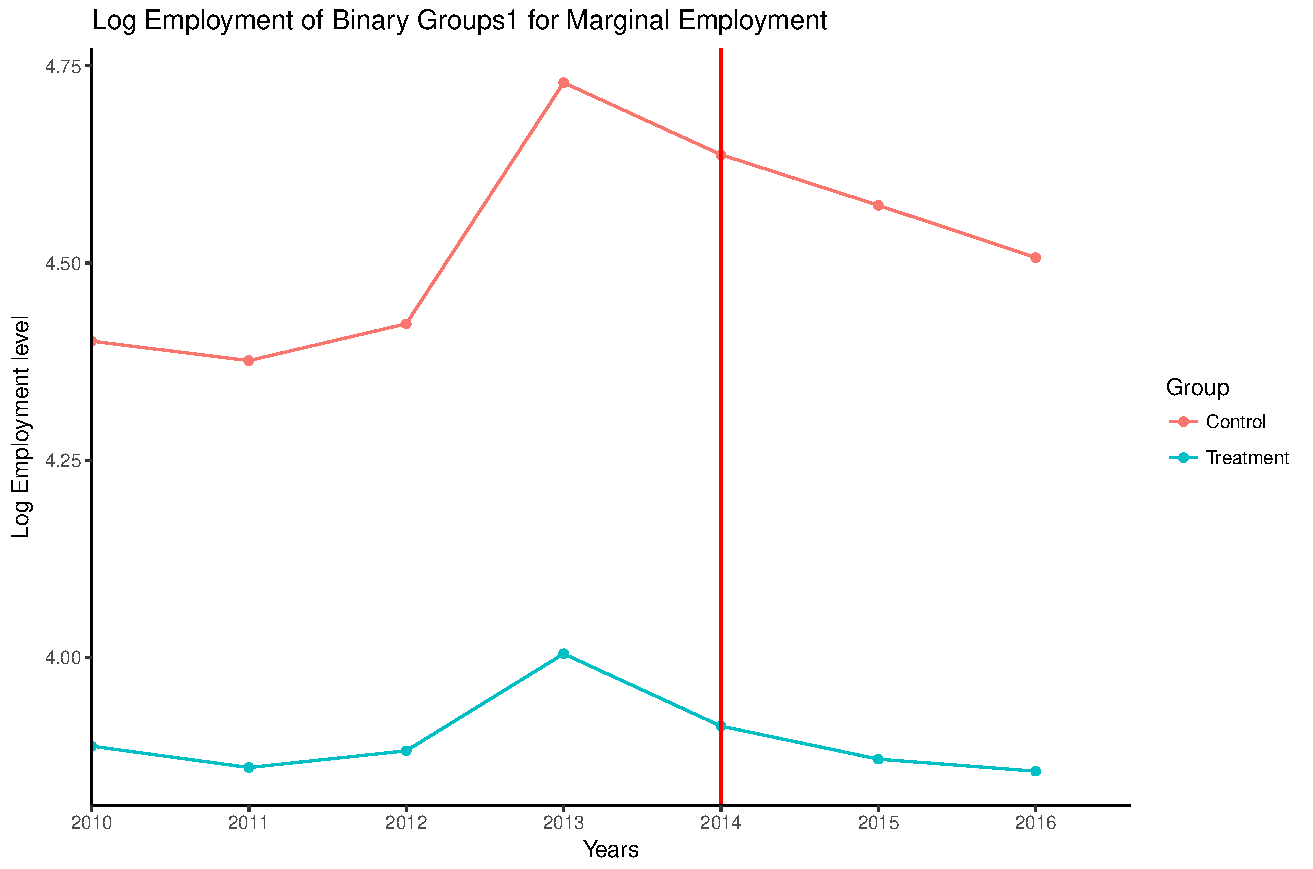
\includegraphics[width=\textwidth]{q6/plot_treatment_ta1marginal.pdf}
\caption{Standard Treatment}
\end{subfigure}
\hfill
\begin{subfigure}[h]{0.5\linewidth}
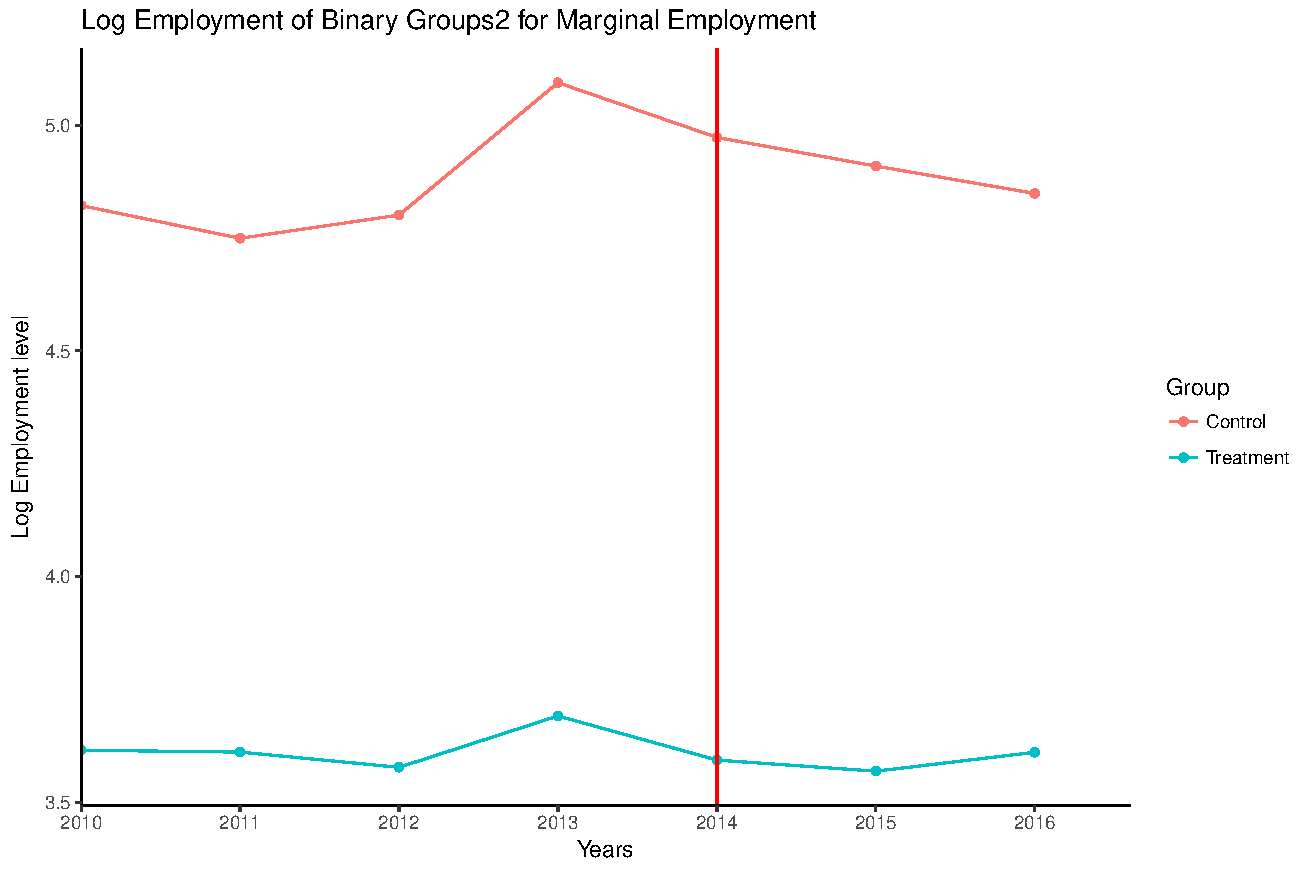
\includegraphics[width=\textwidth]{q6/plot_treatment_ta2marginal.pdf}
\caption{Robust Treatment}
\end{subfigure}%
\caption{Log Marginal Employment}
\label{q6m}
\end{figure}


Figure ~\ref{q6f} compares the log employment of both treatment variations for full time employees. As before, the red marker symbolizes the introduction of the minimum wage. One can see that the log employment levels of the treatment group are smaller than of the control group. Furthermore, there is a decline in levels for both treatment and control group after the minimum wage introduction. However, the decline is only happening in the second period after the introduction for the control group.
\newline
Figure \ref{q6p} compares the log employment for part time employees. Here the plots differ. As one can see there is no decline after the introduction. Instead, there is an increase in Employment.
\newline
Finally, figure \ref{q6m} compares the log employment for marginal employed workers. The graph for the standard treatment displays the strongest decline in employment. Interestingly, the decline seems to be stronger in for the control group.
When comparing all the graphs it seems as the effects differ for the different employment status.


\begin{figure}
\begin{subfigure}[h]{0.33\linewidth}
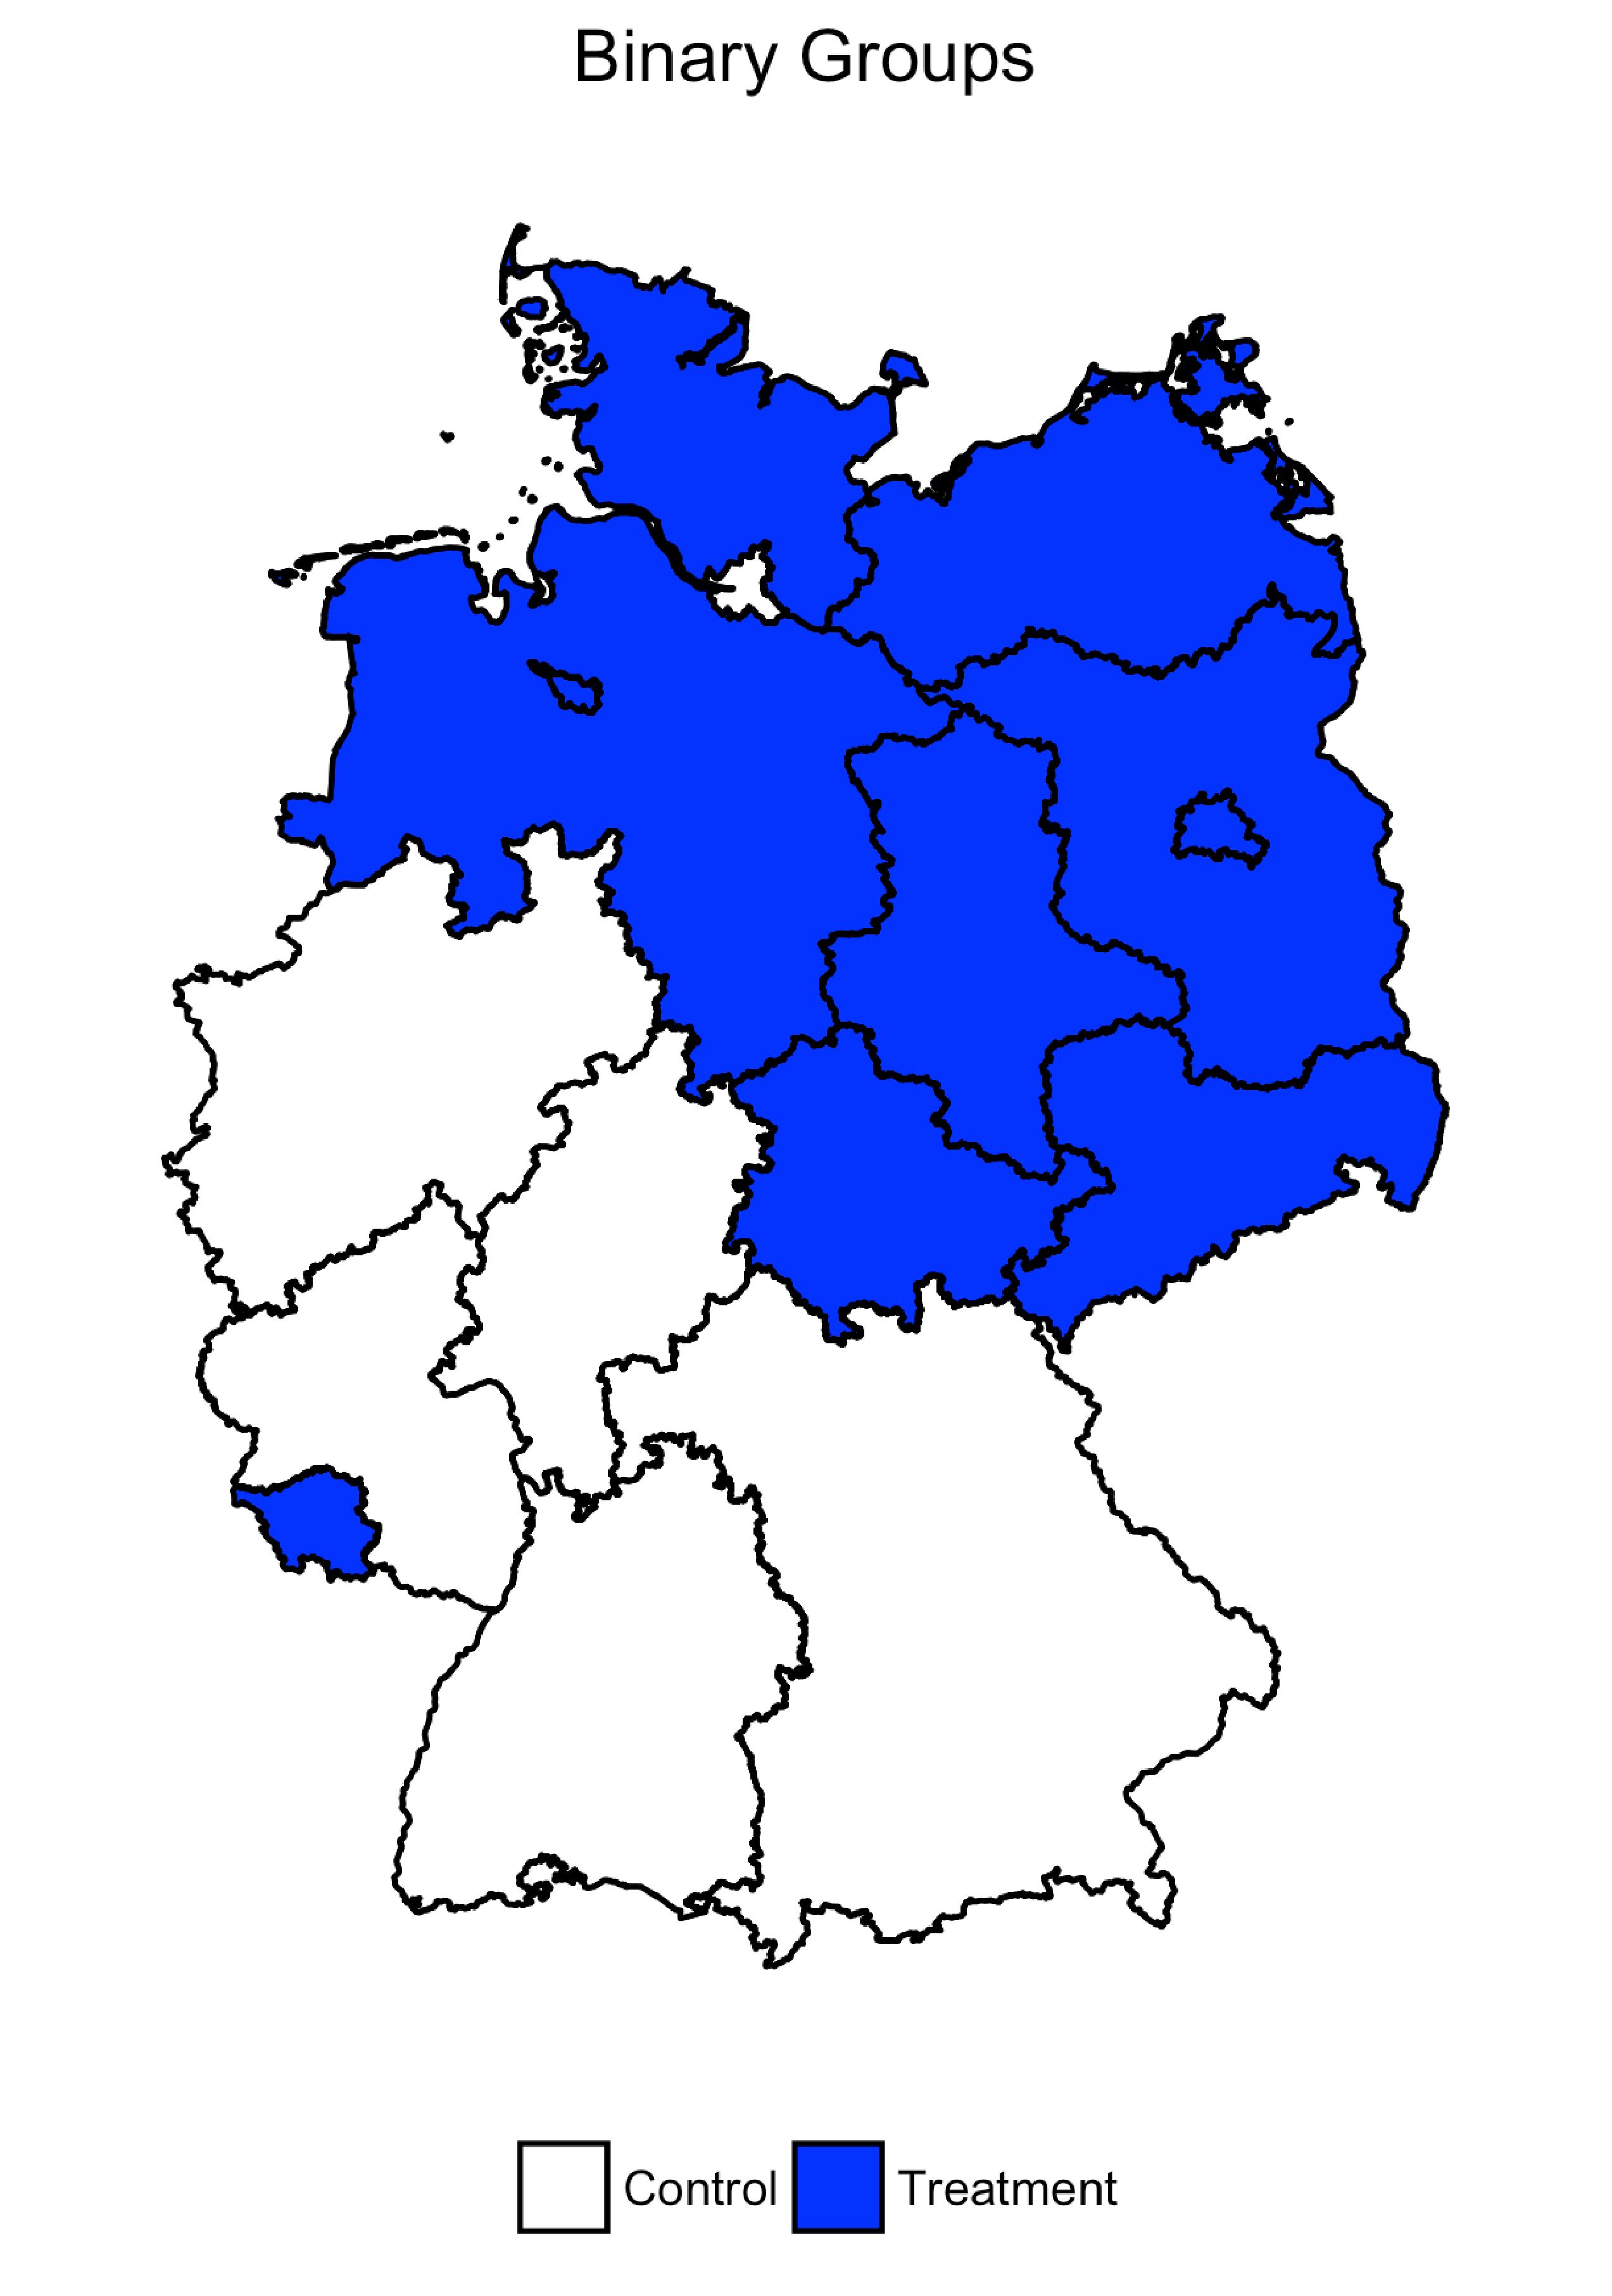
\includegraphics[width=\textwidth]{q6/plot-factor.pdf}
\caption{Binary Groups}
\end{subfigure}
\hfill
\begin{subfigure}[h]{0.33\linewidth}
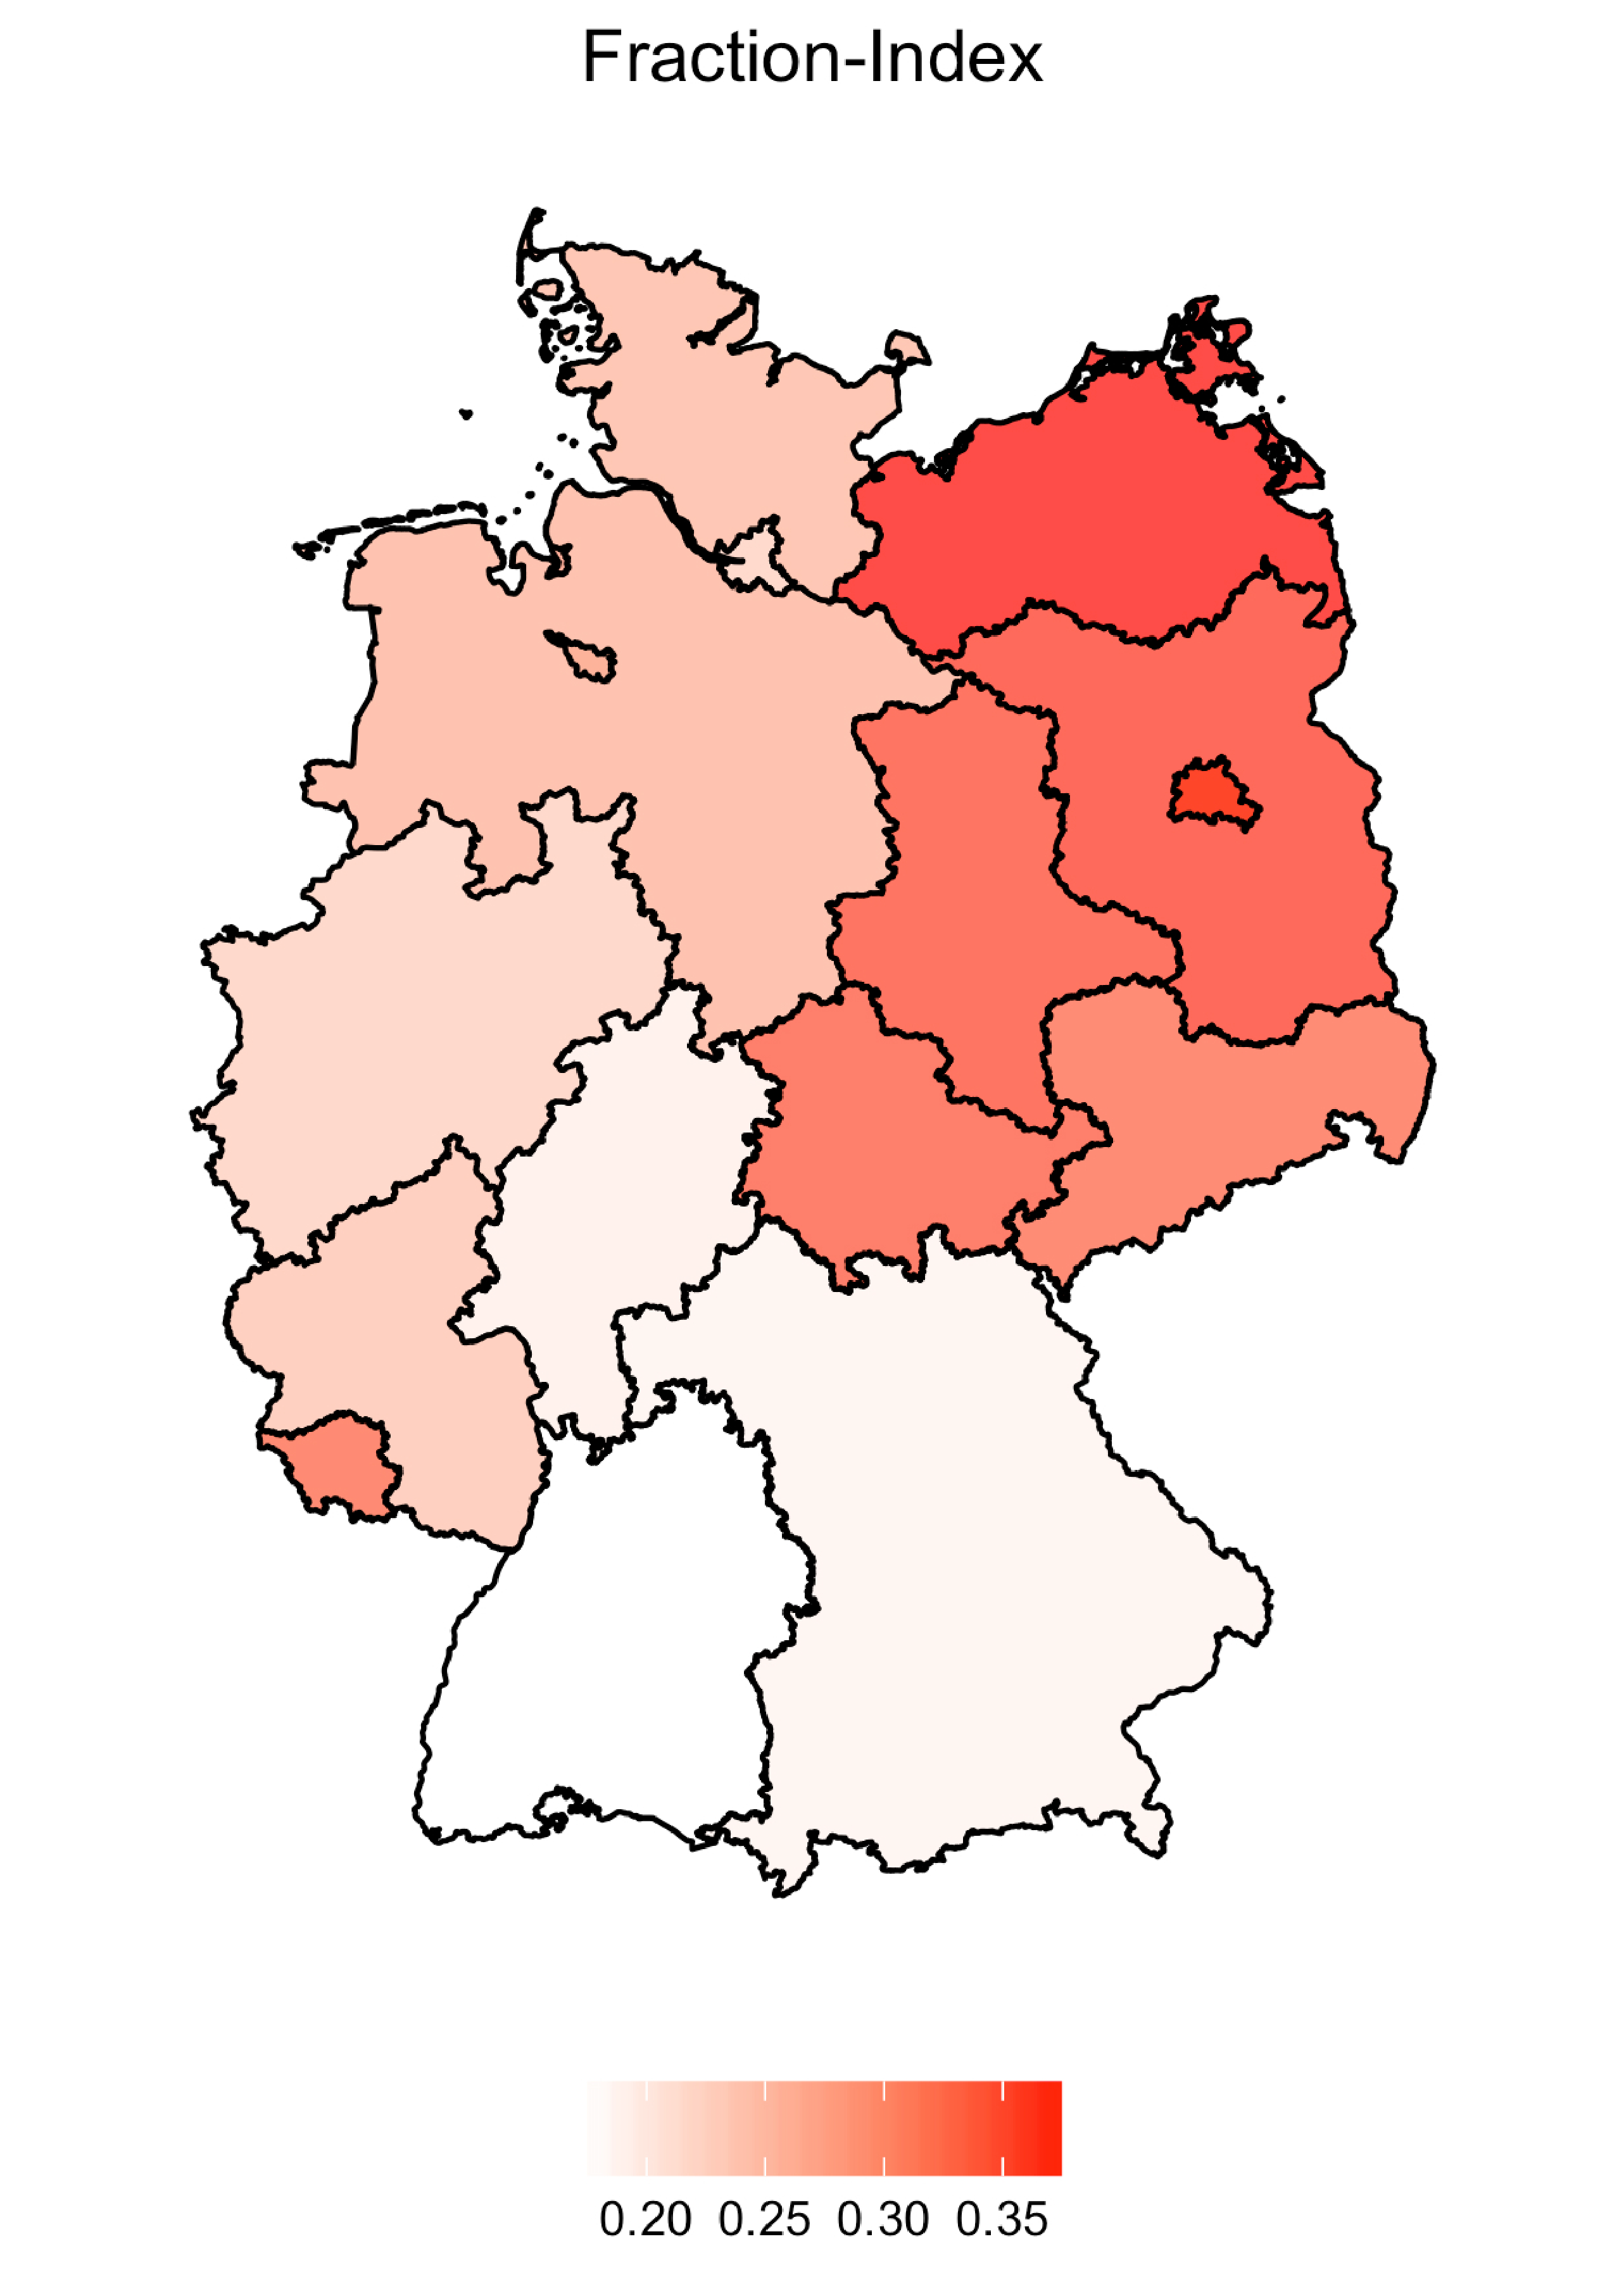
\includegraphics[width=\textwidth]{q6/plot-fraction.pdf}
\caption{Fraction-Index}
\end{subfigure}%
\hfill
\begin{subfigure}[h]{0.33\linewidth}
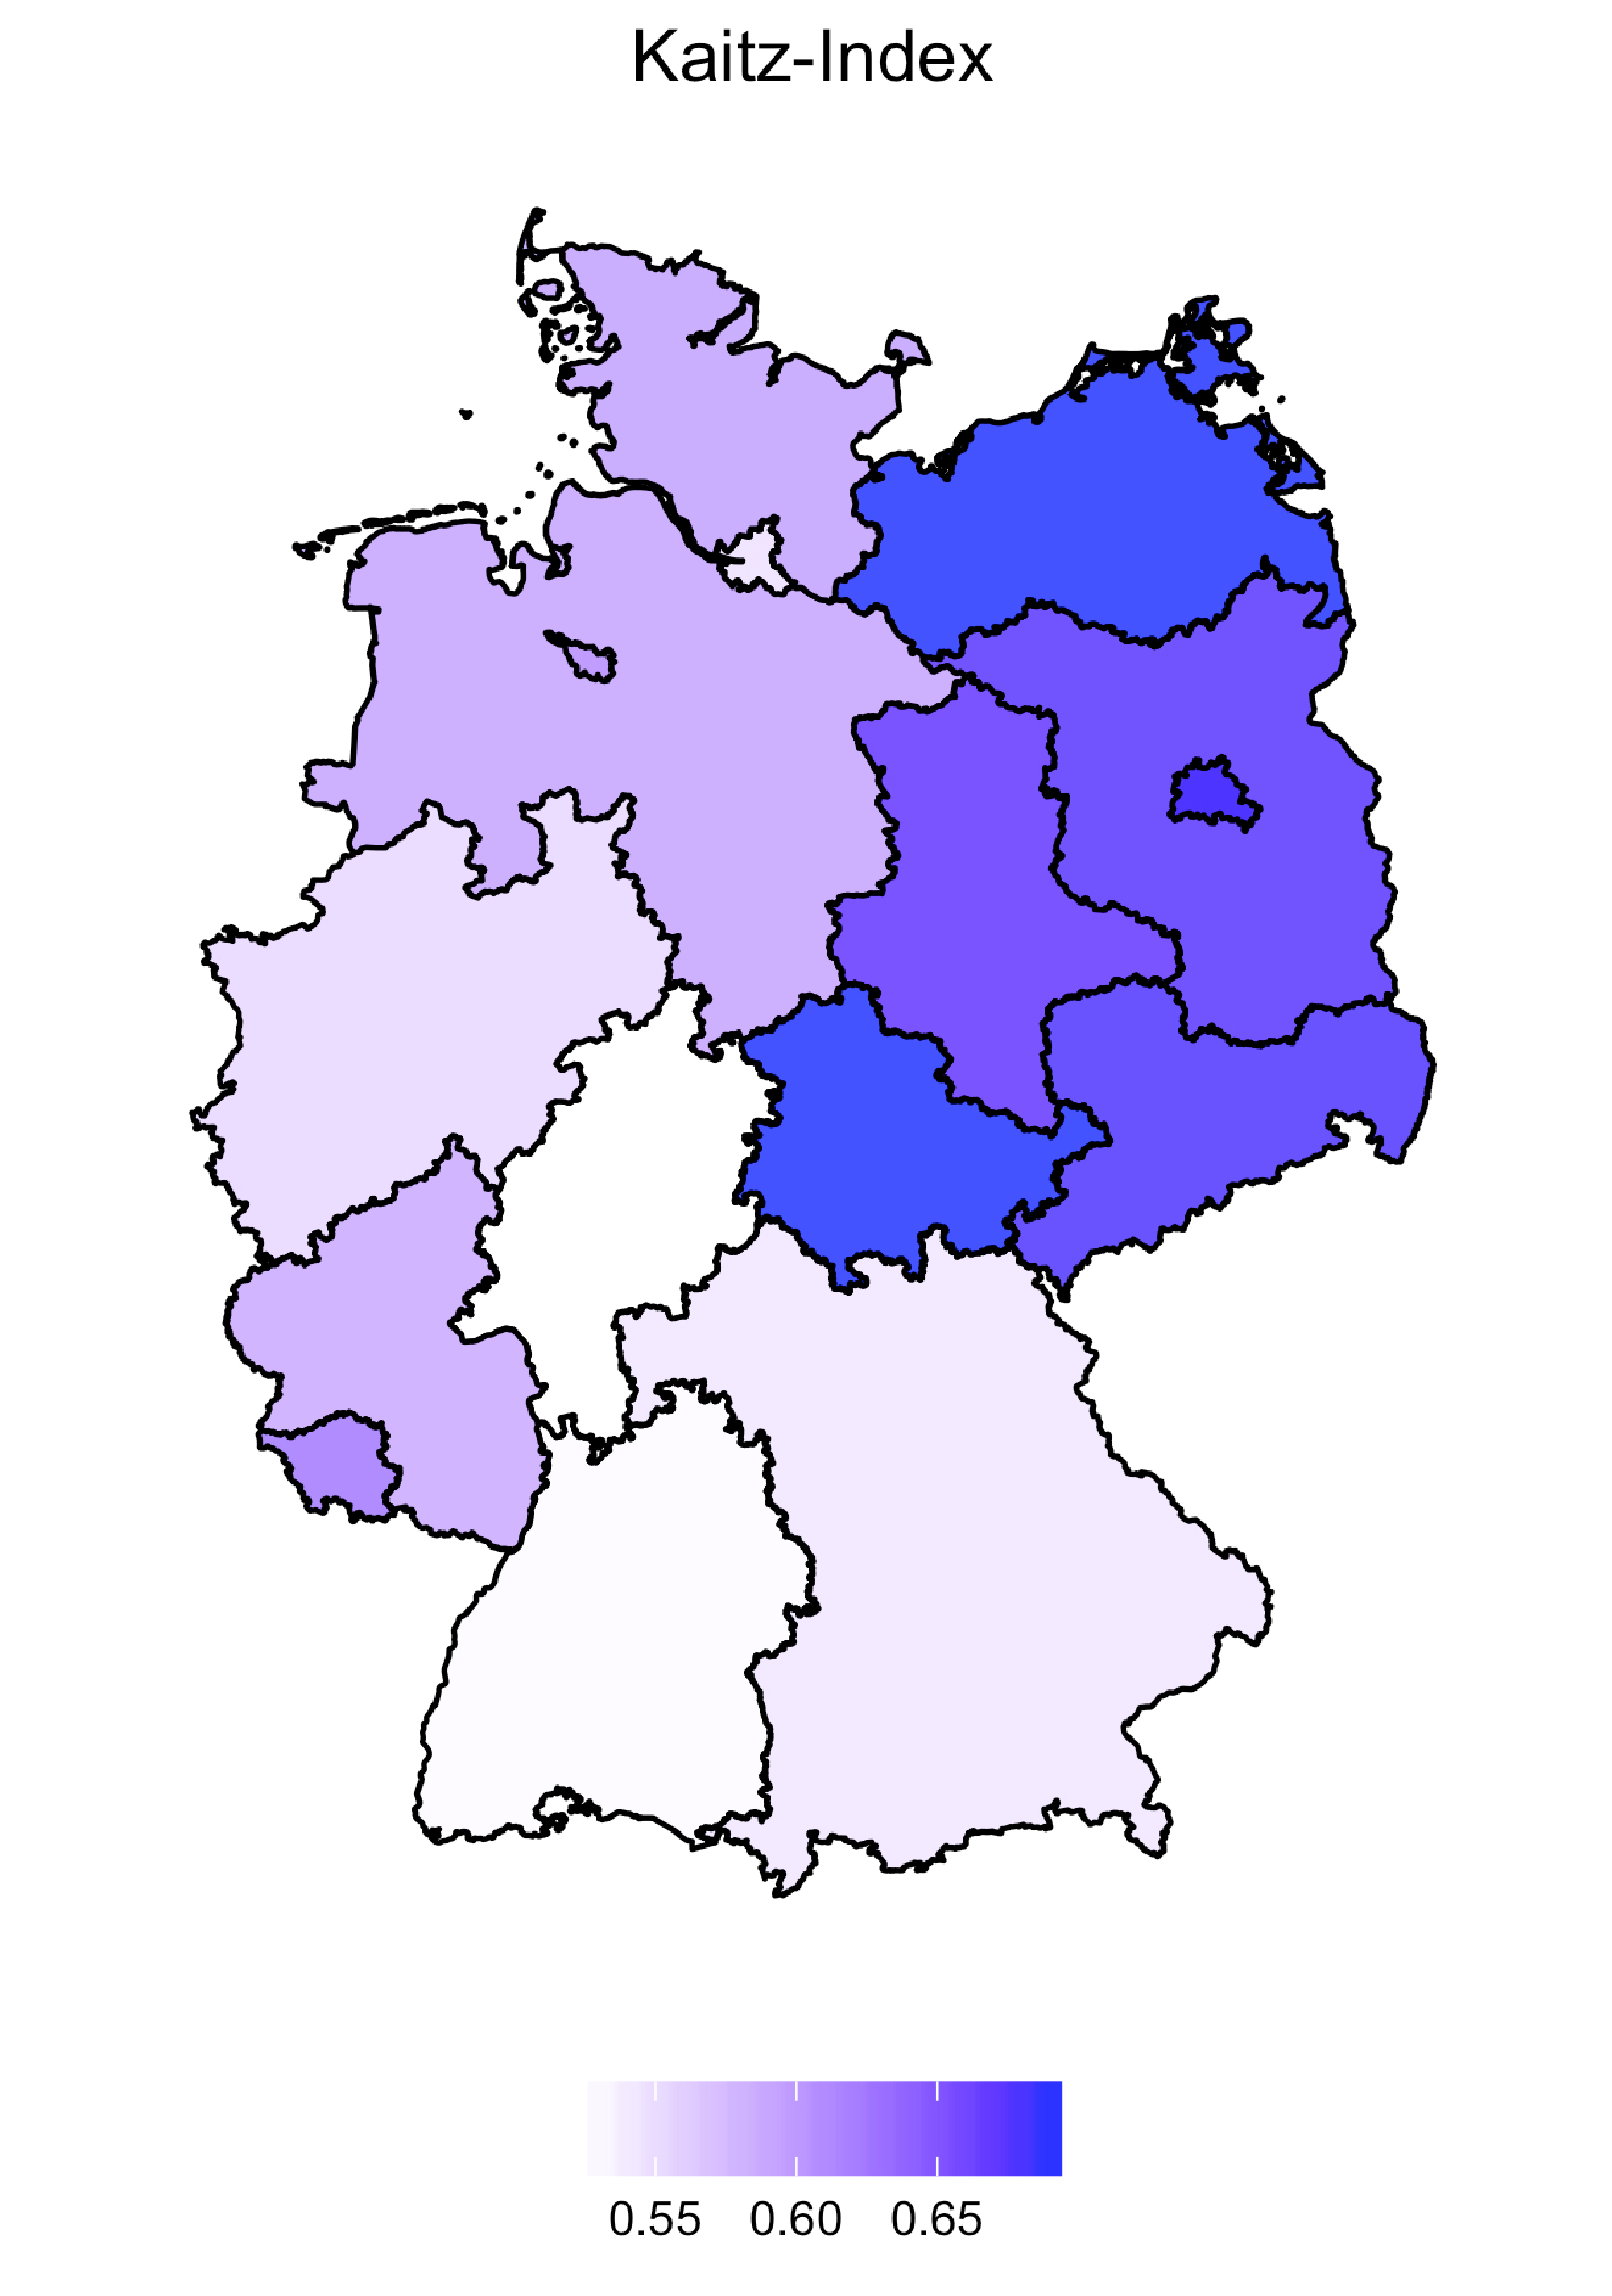
\includegraphics[width=\textwidth]{q6/plot-kaitz.pdf}
\caption{Kaitz-Index}
\end{subfigure}%
\caption{Germany Map}
\label{q6map}
\end{figure}
%
%
Besides the employment graphs, we visualized Fraction and Kaitz Index of the year 2013 using a German map with state borders, as it can be seen in Figure ~\ref{q6map}. One can see a different trend for both indexes, namely that East Germany's wage level is lower and thus more likely to be affected by the minimum wage. This is especially visible, when looking at map, which uses the binary treatment identifier for identification. All eastern states are in the treatment group. Note, that Bremen and Berlin are not supposed to be colored blue. Although, due to the map data it will repaint these areas as they are within another state. 
%
\begin{lstlisting}
\end{lstlisting}
%
%
\section{DiD Estimation}
\subsection{Introduction}
In this section, the goal is to estimate an econometric model which can quantify the effect of the minimum wage introduction on employment. Similar to \cite{schmitz2017effects} and \cite{caliendo2017short} a DiD framework is used. As the data differs and a different region variable is used as well as time variable the model has to be adjusted which will be explained in the following. 
\subsection{Theory}
The DiD approach is a research design for estimating causal effects. The basic idea is to compare the average change of a treatment group, in comparison to the average change control group, which did not receive treatment.
In this case, there are 16 different states and the time measure is in years only. Two different regression models are specified, each similar to either \cite{schmitz2017effects} or \cite{caliendo2017short}.
The first regression model is specified as
\begin{align}
\label{regression1}
E_{i, t} = \gamma_i + \gamma{'}T_t  + \theta_1{'}T_t * Bite_{i, 2014} + \delta X_{i,t} + \nu_{i, t}.
\end{align}
Equation \ref{regression1} is similar to the model used by \cite{caliendo2017short}. $E_{i, t}$ denotes the log employment rate, in this case full-time, part-time or marginal employment in period $t$ for each state $i$, $\gamma_i$ a region fixed-effect, $X_{i,t}$ a set of regional control variables and $\nu_{i, t}$. $T_t$ denotes a year vector and $Bite_{i, 2014}$ is the value of the Fraction and Kaitz Index for state $i$ in year $2014$. Thus, this model is based on the pre-treatment bite in year 2014.

The second model estimates the effect similar, although there are subtly changes in the regression model.
\begin{align}
\label{regression2}
\Delta_{1} E_{i t} = Bite_{i, 2013} * D_t^{MW}*\beta + \sum_t D_t^{year} * \gamma_t + \theta_i + \epsilon_{i t}
\end{align}
Equation \ref{regression2} is by \cite{schmitz2017effects}, though adjusted to make it fit the data. Here, $\Delta_{1} (E_{i t}$ is the log employment rate, $Bite_{i, 2014}$ is the value of the Kaitz Index for state $i$ in year $2013$ and $D_t^{MW}$ is a dummy variable which equals $1$ for all periods after the minimum wage introduction. Moreover, the equation features time fixed effects $\gamma_t$ as well as state fixed effects $\theta_i$. Therefore, this model is based on the pre-treatment bite in year 2013.
%
\subsection{Implementation}
Note that this code is built on the data frame generated in Quantlet6. Accordingly, the quantlets 1, 4, 5 and 6 have to be executed first. \newline
First of all the variables are extracted of interest from the data frame \textbf{analyze\_tc}. This again, is done by a function called \textbf{data\_selector}, which uses the \textbf{select} command from the \textbf{dplyr}-package. The featured variables are mentioned in the following code.
%
\begin{lstlisting}
data_selector = function(analyze_tc) {
    select(filter(analyze_tc), c(Wave, State.of.Residence, Observations, 
    	Fraction, Kaitz, Delta.Log.Full.Employment, 
        Delta.Log.Part.Employment, Delta.Log.Marginal.Employment, 
        binary_treatment1, binary_treatment2, 
        Log.Full.Employment.Rate, Log.Part.Employment.Rate, 									Log.Marginal.Employment.Rate))
}
\end{lstlisting}
The new sub data frame is called \textbf{estimation}.
\begin{lstlisting}
# Apply data selector for sub-dataframe
estimation = data_selector(analyze_tc)
\end{lstlisting}
%
Next, it is necessary to generate all variables needed for the econometric estimation, which is done in two separate steps. First, it is convenient to generate a filter function to subset data depending on the year.
\begin{lstlisting}
data_filter = function(analyze_tc, wave) {
    select(filter(analyze_tc, Wave == wave), c(Wave, State.of.Residence, 
    	Kaitz, Fraction))
}
\end{lstlisting}
Here, the data is filtered by the variable \textbf{Wave}. The function \textbf{data\_filter} is used to subset the data for the years 2013 and 2014. This enables us to subtracts the Kaitz and Fraction Index values of the corresponding years, which are necessary for the estimation as mentioned in Section 8.2.
\begin{lstlisting}
# Create subset for 2013
analyze_2013 = data_filter(analyze_tc, 2013)
\end{lstlisting}
Finally, it is possible to simply add them to the main data frame \textbf{estimation}.
\begin{lstlisting}
estimation$Kaitz.13 = analyze_2013$Kaitz
\end{lstlisting}
This code could further be used to extract the Kaitz and Fraction Index of other years. One simply has to adjust the value in the function \textbf{data\_filter}.
For instance,
\begin{lstlisting}
data_filter(analyze_tc, 2012)
\end{lstlisting}
would subset the data for the year 2012. Second, a data pre-processing function is generated.
Here, all variables needed for the regression estimations and their specifications are generated. In order to generate dummy variables for specific years one first has to convert the variable \textbf{Wave} in numeric values.
\begin{lstlisting}
# Generate numeric variable for years, thus convert the variable wave
x$year = as.numeric(as.character(x$Wave))
\end{lstlisting}
Next, a dummy variable is generated with the \textbf{ifelse} command with the use of the now numeric \textbf{year} variable.
\begin{lstlisting}
# Generate dummy for year for indicator when minimum wage was introduced
x$year15.dummy = ifelse(x$year >= 2015, 1, 0)
\end{lstlisting}
This generates a variable which will be assigned the value \textit{one} if the \textbf{year} variable is \textit{2015} or bigger. Otherwise, the value \textit{zero} will be assigned.
The interaction variables are also generated beforehand. For example, in the second regression the term $Bite_{i, 2013} * D_t^{MW}$ is generated by the following command.
\begin{lstlisting}
# Generate Interaction Variable Kaitz for Schmitz2017
x$DiD.estimator.Kaitz.Schmitz = (x$year15.dummy * x$Kaitz.13)
\end{lstlisting}
Similarly, the interaction variables for the binary treatment and control variables are generated. The exact code for the \textbf{pre\_processing\_estimation} function can be found in the Appendix.
\begin{lstlisting}
# Generate Interaction Variable Binary Treatment Schimtz2017
x$binary1 = (x$binary_treatment1 * x$year15.dummy)

# Generate Control Variables Control for years:
x$year14.dummy = ifelse(x$year >= 2014, 1, 0)    
\end{lstlisting}
Finally, the function is applied to the data frame \textbf{estimation}.
\begin{lstlisting}
# Apply it to data
estimation = pre_processing_estimation(estimation)
\end{lstlisting}
Now the data frame is suited for the estimation. The regressions are specified with the \textbf{plm} command from the \textbf{plm} package. The command is designed to estimate panel data. Using this command is quite convenient as one can simply specify the model structure, such as a fixed effect model.
In detail, a regression is specified in the following way.
\begin{lstlisting}
# Regression 1.2.2: Using Fraction Index and Control Variables
did_1.2.2 = plm(Log.Full.Employment.Rate ~ DiD.estimator.Fraction + 
	Log.Population + Interaction_Fraction_y13 + 
    	Interaction_Fraction_y12, 
	data = estimation, 
    index = c("State.of.Residence", "Wave"), 
    model = "within")
\end{lstlisting}
Here, the log full employment rate is regressed using the Fraction Index as well some control variables. As the data source the data frame \textbf{estimation} is used. The \textbf{index} specification states the indexes $i, t$ thus it have to specify them using \textbf{State.of.Residence} and \textbf{Wave}. Last the model has to be specified. It simply assume a fixed model, thus use the corresponding command \textbf{"within"}.
Different estimation models can now be easily estimated. For instance one is able to change the variable of interest or the regressors.

\subsection{Output}
In total 21 equations are estimated. The following tables display the coefficient values accordingly as well as the standard errors and significance levels.
%
%
%%%% Stargazer Output of Q7 in here%%%
% Table1 
\begin{table}[!htbp] \centering 
  \caption{Effects on Full Time Employment using Kaitz and Fraction Index} 
  \label{RegTable1} 
\begin{tabular}{@{\extracolsep{5pt}}lD{.}{.}{-3} D{.}{.}{-3} D{.}{.}{-3} D{.}{.}{-3} } 
\\[-1.8ex]\hline 
\hline \\[-1.8ex] 
 & \multicolumn{4}{c}{\textit{Dependent variable:}} \\ 
\cline{2-5} 
\\[-1.8ex] & \multicolumn{4}{c}{Panel A: Log Regular Employment Rate} \\ 
 & \multicolumn{2}{c}{Kaitz} & \multicolumn{2}{c}{Fraction} \\ 
\\[-1.8ex] & \multicolumn{1}{c}{(1)} & \multicolumn{1}{c}{(2)} & \multicolumn{1}{c}{(3)} & \multicolumn{1}{c}{(4)}\\ 
\hline \\[-1.8ex] 
 Bite.K x D2015 & -0.184^{***} & -0.192^{***} &  &  \\ 
  & (0.026) & (0.028) &  &  \\ 
  Bite.F x D2015 &  &  & -0.439^{***} & -0.454^{***} \\ 
  &  &  & (0.062) & (0.065) \\ 
  Population(log,t) &  & -0.469^{***} &  & -0.471^{***} \\ 
  &  & (0.083) &  & (0.082) \\ 
  Bite.K x D2013 &  & -0.003 &  &  \\ 
  &  & (0.034) &  &  \\ 
  Bite.K x D2012 &  & 0.019 &  &  \\ 
  &  & (0.034) &  &  \\ 
  Bite.F x D2013 &  &  &  & -0.022 \\ 
  &  &  &  & (0.080) \\ 
  Bite.F x D2012 &  &  &  & 0.051 \\ 
  &  &  &  & (0.079) \\ 
 \hline \\[-1.8ex] 
Observations & \multicolumn{1}{c}{112} & \multicolumn{1}{c}{112} & \multicolumn{1}{c}{112} & \multicolumn{1}{c}{112} \\ 
R$^{2}$ & \multicolumn{1}{c}{0.343} & \multicolumn{1}{c}{0.514} & \multicolumn{1}{c}{0.344} & \multicolumn{1}{c}{0.518} \\ 
Adjusted R$^{2}$ & \multicolumn{1}{c}{0.233} & \multicolumn{1}{c}{0.413} & \multicolumn{1}{c}{0.234} & \multicolumn{1}{c}{0.419} \\ 
\hline 
\hline \\[-1.8ex] 
\textit{Note:}  & \multicolumn{4}{r}{$^{*}$p$<$0.1; $^{**}$p$<$0.05; $^{***}$p$<$0.01} \\ 
\end{tabular} 
\end{table} 
% Table2
\begin{table}[!htbp] \centering 
  \caption{Effects on Part Time Employment using Kaitz and Fraction Index} 
  \label{RegTable2} 
\begin{tabular}{@{\extracolsep{5pt}}lD{.}{.}{-3} D{.}{.}{-3} D{.}{.}{-3} D{.}{.}{-3} } 
\\[-1.8ex]\hline 
\hline \\[-1.8ex] 
 & \multicolumn{4}{c}{\textit{Dependent variable:}} \\ 
\cline{2-5} 
\\[-1.8ex] & \multicolumn{4}{c}{Panel B: Log Part Time Employment Rate} \\ 
 & \multicolumn{2}{c}{Kaitz} & \multicolumn{2}{c}{Fraction} \\ 
\\[-1.8ex] & \multicolumn{1}{c}{(1)} & \multicolumn{1}{c}{(2)} & \multicolumn{1}{c}{(3)} & \multicolumn{1}{c}{(4)}\\ 
\hline \\[-1.8ex] 
 Bite.K x D2015 & -0.023 & -0.091^{***} &  &  \\ 
  & (0.031) & (0.033) &  &  \\ 
  Bite.F x D2015 &  &  & -0.056 & -0.215^{***} \\ 
  &  &  & (0.073) & (0.079) \\ 
  Population(log,t) &  & -0.359^{***} &  & -0.341^{***} \\ 
  &  & (0.099) &  & (0.099) \\ 
  Bite.K x D2013 &  & 0.043 &  &  \\ 
  &  & (0.040) &  &  \\ 
  Bite.K x D2012 &  & 0.104^{**} &  &  \\ 
  &  & (0.040) &  &  \\ 
  Bite.F x D2013 &  &  &  & 0.099 \\ 
  &  &  &  & (0.096) \\ 
  Bite.F x D2012 &  &  &  & 0.235^{**} \\ 
  &  &  &  & (0.096) \\ 
 \hline \\[-1.8ex] 
Observations & \multicolumn{1}{c}{112} & \multicolumn{1}{c}{112} & \multicolumn{1}{c}{112} & \multicolumn{1}{c}{112} \\ 
R$^{2}$ & \multicolumn{1}{c}{0.006} & \multicolumn{1}{c}{0.241} & \multicolumn{1}{c}{0.006} & \multicolumn{1}{c}{0.229} \\ 
Adjusted R$^{2}$ & \multicolumn{1}{c}{-0.162} & \multicolumn{1}{c}{0.085} & \multicolumn{1}{c}{-0.161} & \multicolumn{1}{c}{0.070} \\ 
\hline 
\hline \\[-1.8ex] 
\textit{Note:}  & \multicolumn{4}{r}{$^{*}$p$<$0.1; $^{**}$p$<$0.05; $^{***}$p$<$0.01} \\ 
\end{tabular} 
\end{table} 
% Table3
\begin{table}[!htbp] \centering 
  \caption{Effects on Marginal Employment using Kaitz and Fraction Index} 
  \label{RegTable3} 
\begin{tabular}{@{\extracolsep{5pt}}lD{.}{.}{-3} D{.}{.}{-3} D{.}{.}{-3} D{.}{.}{-3} } 
\\[-1.8ex]\hline 
\hline \\[-1.8ex] 
 & \multicolumn{4}{c}{\textit{Dependent variable:}} \\ 
\cline{2-5} 
\\[-1.8ex] & \multicolumn{4}{c}{Panel C: Log Marginal Employment Rate} \\ 
 & \multicolumn{2}{c}{Kaitz} & \multicolumn{2}{c}{Fraction} \\ 
\\[-1.8ex] & \multicolumn{1}{c}{(1)} & \multicolumn{1}{c}{(2)} & \multicolumn{1}{c}{(3)} & \multicolumn{1}{c}{(4)}\\ 
\hline \\[-1.8ex] 
 Bite.K x D2015 & -0.014 & -0.163^{***} &  &  \\ 
  & (0.053) & (0.059) &  &  \\ 
  Bite.F x D2015 &  &  & -0.027 & -0.361^{**} \\ 
  &  &  & (0.127) & (0.141) \\ 
  Population(log,t) &  & -0.197 &  & -0.159 \\ 
  &  & (0.178) &  & (0.179) \\ 
  Bite.K x D2013 &  & 0.233^{***} &  &  \\ 
  &  & (0.072) &  &  \\ 
  Bite.K x D2012 &  & 0.023 &  &  \\ 
  &  & (0.072) &  &  \\ 
  Bite.F x D2013 &  &  &  & 0.526^{***} \\ 
  &  &  &  & (0.173) \\ 
  Bite.F x D2012 &  &  &  & 0.039 \\ 
  &  &  &  & (0.173) \\ 
 \hline \\[-1.8ex] 
Observations & \multicolumn{1}{c}{112} & \multicolumn{1}{c}{112} & \multicolumn{1}{c}{112} & \multicolumn{1}{c}{112} \\ 
R$^{2}$ & \multicolumn{1}{c}{0.001} & \multicolumn{1}{c}{0.187} & \multicolumn{1}{c}{0.0005} & \multicolumn{1}{c}{0.166} \\ 
Adjusted R$^{2}$ & \multicolumn{1}{c}{-0.168} & \multicolumn{1}{c}{0.019} & \multicolumn{1}{c}{-0.168} & \multicolumn{1}{c}{-0.007} \\ 
\hline 
\hline \\[-1.8ex] 
\textit{Note:}  & \multicolumn{4}{r}{$^{*}$p$<$0.1; $^{**}$p$<$0.05; $^{***}$p$<$0.01} \\ 
\end{tabular} 
\end{table} 
% Table4
\begin{table}[!htbp] \centering 
  \caption{Effects on Employment Outcomes using Kaitz2013} 
  \label{RegTable4} 
\begin{tabular}{@{\extracolsep{5pt}}lD{.}{.}{-3} D{.}{.}{-3} D{.}{.}{-3} } 
\\[-1.8ex]\hline 
\hline \\[-1.8ex] 
 & \multicolumn{3}{c}{Panel D: Log Employment Status} \\ 
\cline{2-4} 
 & \multicolumn{1}{c}{Full} & \multicolumn{1}{c}{Part} & \multicolumn{1}{c}{Marginal} \\ 
\\[-1.8ex] & \multicolumn{1}{c}{(1)} & \multicolumn{1}{c}{(2)} & \multicolumn{1}{c}{(3)}\\ 
\hline \\[-1.8ex] 
 Bite x D2015 & 0.248 & 0.361 & 0.039 \\ 
  & (0.506) & (0.488) & (0.532) \\ 
  Linear Trend & 44.564 & 137.026 & 99.045 \\ 
  & (162.713) & (156.841) & (171.054) \\ 
  Quadratic Trend & -0.011 & -0.034 & -0.025 \\ 
  & (0.040) & (0.039) & (0.043) \\ 
 \hline \\[-1.8ex] 
Observations & \multicolumn{1}{c}{112} & \multicolumn{1}{c}{112} & \multicolumn{1}{c}{112} \\ 
R$^{2}$ & \multicolumn{1}{c}{0.013} & \multicolumn{1}{c}{0.008} & \multicolumn{1}{c}{0.007} \\ 
Adjusted R$^{2}$ & \multicolumn{1}{c}{-0.178} & \multicolumn{1}{c}{-0.184} & \multicolumn{1}{c}{-0.185} \\ 
\hline 
\hline \\[-1.8ex] 
\textit{Note:}  & \multicolumn{3}{r}{$^{*}$p$<$0.1; $^{**}$p$<$0.05; $^{***}$p$<$0.01} \\ 
\end{tabular} 
\end{table} 
% Table5
\begin{table}[!htbp] \centering 
  \caption{Effects on Employment Outcomes using standard Binary Treatment} 
  \label{RegTable5} 
\begin{tabular}{@{\extracolsep{5pt}}lD{.}{.}{-3} D{.}{.}{-3} D{.}{.}{-3} } 
\\[-1.8ex]\hline 
\hline \\[-1.8ex] 
 & \multicolumn{3}{c}{Panel E: Log Employment Status} \\ 
\cline{2-4} 
 & \multicolumn{1}{c}{Full} & \multicolumn{1}{c}{Part} & \multicolumn{1}{c}{Marginal} \\ 
\\[-1.8ex] & \multicolumn{1}{c}{(1)} & \multicolumn{1}{c}{(2)} & \multicolumn{1}{c}{(3)}\\ 
\hline \\[-1.8ex] 
 Treated x 2015 & -0.032 & 0.047 & -0.019 \\ 
  & (0.178) & (0.171) & (0.186) \\ 
  & & & \\ 
\hline \\[-1.8ex] 
Observations & \multicolumn{1}{c}{112} & \multicolumn{1}{c}{112} & \multicolumn{1}{c}{112} \\ 
R$^{2}$ & \multicolumn{1}{c}{0.0003} & \multicolumn{1}{c}{0.001} & \multicolumn{1}{c}{0.0001} \\ 
Adjusted R$^{2}$ & \multicolumn{1}{c}{-0.168} & \multicolumn{1}{c}{-0.167} & \multicolumn{1}{c}{-0.168} \\ 
\hline 
\hline \\[-1.8ex] 
\textit{Note:}  & \multicolumn{3}{r}{$^{*}$p$<$0.1; $^{**}$p$<$0.05; $^{***}$p$<$0.01} \\ 
\end{tabular} 
\end{table} 
% Table6
\begin{table}[!htbp] \centering 
  \caption{Effects on Employment Outcomes using Robust Binary Treatment} 
  \label{RegTable6} 
\begin{tabular}{@{\extracolsep{5pt}}lD{.}{.}{-3} D{.}{.}{-3} D{.}{.}{-3} } 
\\[-1.8ex]\hline 
\hline \\[-1.8ex] 
 & \multicolumn{3}{c}{Panel F: Log Employment Status} \\ 
\cline{2-4} 
 & \multicolumn{1}{c}{Full} & \multicolumn{1}{c}{Part} & \multicolumn{1}{c}{Marginal} \\ 
\\[-1.8ex] & \multicolumn{1}{c}{(1)} & \multicolumn{1}{c}{(2)} & \multicolumn{1}{c}{(3)}\\ 
\hline \\[-1.8ex] 
 Treated x 2015 & 0.036 & 0.124 & 0.096 \\ 
  & (0.207) & (0.196) & (0.199) \\ 
  & & & \\ 
\hline \\[-1.8ex] 
Observations & \multicolumn{1}{c}{84} & \multicolumn{1}{c}{84} & \multicolumn{1}{c}{84} \\ 
R$^{2}$ & \multicolumn{1}{c}{0.0004} & \multicolumn{1}{c}{0.006} & \multicolumn{1}{c}{0.003} \\ 
Adjusted R$^{2}$ & \multicolumn{1}{c}{-0.169} & \multicolumn{1}{c}{-0.162} & \multicolumn{1}{c}{-0.165} \\ 
\hline 
\hline \\[-1.8ex] 
\textit{Note:}  & \multicolumn{3}{r}{$^{*}$p$<$0.1; $^{**}$p$<$0.05; $^{***}$p$<$0.01} \\ 
\end{tabular} 
\end{table} 
\begin{lstlisting}
\end{lstlisting}
 %
 %
 %
Table \ref{RegTable1} displays the regression estimates of the minimum wage introduction on full time employment. In detail, it combines the estimations using both Kaitz and Fraction Index of the year 2014. Moreover, a baseline is estimated as well as a more complex model using control variables for the population and several interaction terms, in detail, dummy variables of the previous year times the index. According to \cite{caliendo2017short} this controls for possible anticipation effects. It can be seen that in all four different specifications, the minimum wage introduction has a significant negative effect on regular employment. Furthermore, there seem to be no anticipation effects, as these control variables are all insignificant. \newline
Table \ref{RegTable2} and \ref{RegTable3} are similar and display the estimation results for part time and marginal employment, respectively. For both employment statuses, the baseline models estimate an insignificant negative effect of minimum wage introduction. Moreover, some of control variables are significant, indicating an anticipation effect for part time and marginal employment. Although it is surprising that they have a positive impact. \newline
Table \ref{RegTable4} displays the coefficients of the estimation similar to \cite{schmitz2017effects}, while \ref{RegTable5} and \ref{RegTable6} make use of the standart and robust binary treatment identifier. The results are surprising as in all specifications the effects are insignificant. Especially, the results of \ref{RegTable5} appear strange, as it estimates some effects in the opposite way. Thus, this could indicate that the minimum wage introduction had no significant effect on employment, or that our regression model might be wrongly specified.

\section{Statistical Tests}
\subsection{Introduction}
In econometrics, it is often very difficult to specify a model correctly. Often, problems arise because the estimation might be biased, inconsistent or inefficient. For instance, if heteroscedasticity occurs an estimation might be inefficient as the true variance and covariance is underestimated, depending on the estimation model. Therefore, this section focuses on several tests, which control for the properties of an econometric model. The goal is to write a function which correctly specifies a panel data model. The following tests will be addressed:
\begin{itemize}
\item Hausman specification test
\item Testing for time-fixed effects
\item Breusch-Pagan Lagrange multiplier (LM) for cross-sectional dependence
\item Breusch-Godfrey/Wooldridge test for serial correlation
\item Breusch-Pagan test for heteroscedasticity
\end{itemize}

\subsection{Theory}
This section will quickly cover the test properties.
The Hausman specification test evaluates the consistency of an estimator compared to an alternative, the test evaluates the consistency of an estimator when compared to an alternative, less efficient estimator which is already known to be consistent. It can also be used to differentiate between a fixed effects model compared to a random effects model. Thus, it basically tests whether the unique errors are correlated with the regressors. The null hypothesis is they are not, hence a random effect model would be preferred under the null hypothesis. \newline
Testing for time-fixed effects evaluates whether time-fixed effects are needed to be specified in a model. Rejecting the null hypothesis with a $p-value < 0.05$ means that time-fixed effects are needed. The LM test evaluates the cross-sectional dependence, thus whether there might be spatial or spill over effects. Furthermore, this dependence can arise due to unobserved or unobservable common factors. Again, we reject the null hypothesis with a $p-value < 0.05$ and so cross-sectional dependence is a problem of the estimation. Next, the test for serial correlation evaluates whether error terms from different time-periods are correlated, hence the error term is serially correlated. As before, a $p-value < 0.05$ leads to the rejection of the null hypothesis, so a serial correlation issue has to be made. Finally, a test for heteroscedasticity is conducted. 


\subsection{Implementation}
All tests are coded within one function, called \textbf{estimate\_appropriate\_model}. This function makes use of the inputs of a fixed effects model (fe) and a random effects model (re). First, the tests are run subsequently. The p-values are used which are assigned and generate a \textbf{testvalues} vector, which stores all test results. In detail, it makes use of the corresponding p-values of each specific test. Whenever $p-value < 0.05$ the value \textit{one} will be assigned to the vector, as can be seen in the following code.
\begin{lstlisting}
currvalue = ifelse(TimeFixedEffectsTest$p.value < 0.05, 1, 0)
testvalues = c(testvalues, currvalue)
\end{lstlisting}
Second, depending on the values of the \textbf{testvalues} vector, the function displays the correct model and estimates the model with robust standard errors if necessary. This is achieved with a slope which steps through the different values of the vector.
\begin{lstlisting}
# Estimate correct coefficients
    if (testvalues[1] == 0) {
        if (testvalues[6] == 0) {
            output[1] = "Random effect model without heteroskedasticity"
            output[[2]] = coeftest(re)
\end{lstlisting}
If the first and sixth value of the \textbf{testvalue} vector equal \textit{zero} the model would be correctly specified as a random effect model without heteroskedasticity and the coefficients would not have to be adjusted by robust standard errors.

\begin{lstlisting}
\end{lstlisting}

\subsection{Testing}
The function is tested using two regressions of Quantlet7.
As all regressions were estimated by a fixed effect model, it has to correctly specify the corresponding random effect model.

\begin{lstlisting}
fixed.1 = did_2.2.2
random.1 = plm(Log.Part.Employment.Rate ~ DiD.estimator.Fraction + 
	Log.Population + Interaction_Fraction_y13 + 
    	Interaction_Fraction_y12, 
    	data = estimation, 
    	index = c("State.of.Residence", "Wave"), model = "random")
        
fixed.2 = did_4.2
random.2 = plm(Delta.Log.Full.Employment ~ binary1, data = estimation, 
index = c("State.of.Residence", 
    "Wave"), model = "random")
\end{lstlisting}
After, one simply has to apply the function.
\begin{lstlisting}
# Estimate the appropriate model
estimate_appropriate_model(fixed.1, random.1)
\end{lstlisting}
 The newly estimated model differs from the original model \textbf{did\_2.2.2} which can be compared with the \textbf{summary} command.

The same occurs when checking for the second example.
\begin{lstlisting}
# Estimate the appropriate model
estimate_appropriate_model(fixed.2, random.2)
# Compare with original estimation
summary(fixed.2)
\end{lstlisting}
This indicates that the models specified in Quantlet7 are not ideal and could be optimized for a better estimation.

\section{Conclusion}
All in all, we were able to find out a lot about the effect of the minimum wage introduction on employment in Germany. We tried to code as flexible and dynamic as possible, such that future adjustments, i.e. using newer data or making slight changes to functions can be applied in a smooth way. While firstly analyzing the earning and employment structure descriptively and graphically for a specific wave of the SOEP data, we later analyzed the data around the years before and after the minimum wage introduction. Graphically, it seemed as the minimum wage introduction had an effect on employment. However, using an econometric panel data estimation the effect is ambiguous, as some estimation were significant while others were not. This raises the question, whether some of our models might be badly specified. Especially, the statistical tests performed in the last section, support the theory of not ideal specified models. While we, deliberately tried to follow the estimation strategies of \cite{schmitz2017effects} and \cite{caliendo2017short}, we were not able to replicate their findings perfectly. In our opinion, this is mainly due to the different datasets used. We had to make some changes, as our sample size and time variables differed. With a richer dataset for each wave, we would have been able to focus on a more detailed regional level as well. All in all, this project was an eyeopener about the possibilities on how to conduct an empirical study with a statistical program.
\newpage
\section{References}
\bibliographystyle{plainnat}
\bibliography{main}
\newpage
\section{Appendix}
\subsection{Code for Quantlet 1: SOEPQ1\_ImportPrepareData}
\begin{lstlisting}[numbers=none]
## Quantlet 1 - ImportPrepareData Load Packages used in Q1
library(foreign)
library(stringr)
library(data.table)

# Make Sure you check the Working Dir so that the code works flawless!
getwd()
# Otherwise Set the Working Directory -> setwd('/Your/Path/to/Happiness')

### IMPORT, MERGE AND CLEAN ALL DATA 
### We need two iterators: i is to step through the list of years,
### beginning with k is always one digit higher than i as it reads the 
second column of the feature
### selection list (the first column is the label)
i = 1  # iterator to step through the list of years
k = 2  # iterator to step through the columns in variable list
# List all directories within the input data, non-recursive
list_dirs = list.dirs(path = "SOEPQ1_ImportPrepareData/input-data", 
recursive = FALSE)
# Extract year name of the directories, so the last 4 digits
list_years = str_sub(list_dirs, -4)
# Create Variable names for every merged year based on merged[year]
list_varnames = paste("merged", list_years, sep = "")
# Load the variable list we cleaned manually in Excel as CSV
soep_selection = read.table("SOEPQ1_ImportPrepareData/variable-selection/
soep-var-selection.csv", header = TRUE, sep = ";", check.names = FALSE)
# Get all Labels, unfiltered
labels = soep_selection[, 1]
# Create a vector to put object names of all years in it
datalist = c()

# Loop through all the years, import the data, merge, clean and label them
for (years in list_years) {
    # Define Current List of import data based on the 'i' value
    list_files = list.files(path = list_dirs[i], pattern = "", 
    full.names = TRUE)
    # Import all the data from the current list with the read.dta-Function 
    (part of foreign package) for
    # SPSS-Files
    list_import = lapply(list_files, read.dta)
    # Merge it into one file
    data_merged = Reduce(function(x, y) merge(x, y, by = "persnr", 
    all.x = TRUE), list_import)
    # Cut the .x and .y values from the merge process, so that we have 
    clean column names
    colnames(data_merged) = gsub("\\.x|\\.y", "", colnames(data_merged))
    # Get the variable list of the current year
    current_list = sort(soep_selection[, k])
    # ONLY take the data shortlisted for the current year
    cleaned = data_merged[, which(names(data_merged) %in% current_list 
    == TRUE)]
    # Select the Label Column and the Variable Column of the current Year
    soep_subcrit = c(1, k)
    # Subset Variable list so that only label and the current year exist
    soep_selection_sub = soep_selection[soep_subcrit]
    # Delete NA-Values from the list
    soep_selection_sub = na.omit(soep_selection_sub)
    # Create a subset of the clean labels, where all codenames match,
    # to make sure that the labels arecorrect
    clean_labels = subset(soep_selection_sub, sort(soep_selection_sub[, 2]) 
    == sort(names(cleaned)))
    # Order Dataframe alphabetically
    clean_sorted = cleaned[, order(names(cleaned))]
    # Order Frame with the Labels based on the ID
    ordered_colnames = clean_labels[order(clean_labels[2]), ]
    # Label the columns properly
    colnames(clean_sorted) = ordered_colnames[, 1]
    # Assign data_merged to current merge[year]
    assign(list_varnames[i], clean_sorted)
    # Add Year Variable to a list so that we can access all years by a loop
    datalist = c(datalist, list_varnames[i])
    # Update our variables for the next round
    i = i + 1
    k = k + 1
}

# Merge all data into one dataframe and add a column with the respective 
year, called 'Wave' 
# Create a new dataframe
merged_all = data.frame(matrix(ncol = nrow(soep_selection), nrow = 0))
# Name the dataframe using the first column of the csv
colnames(merged_all) <- soep_selection[, 1]
# Add 'Wave' column to the dataframe
merged_all$Wave = numeric(nrow(merged_all))
# Iterator to step through the years
z = 1
# For loop adding data of every year to the data frame
for (years in c(datalist)) {
    # Get current year for the Wave column
    current_year = list_years[z]
    # Get dataset of the current year
    current_data = get(datalist[z])
    # Repeat current year to fill the column 'Wave' of the respective year
    Wave = rep(current_year, nrow(current_data))
    # Add year-value to the 'Wave' column
    current_data = cbind(Wave, current_data)
    # Add the data to the merge dataframe
    merged_all = rbindlist(list(merged_all, current_data), fill = TRUE)
    # Iterator one up
    z = z + 1
}  # END OF FOR-LOOP

# Removes Spaces in Variable Names and substitues with a . - 
Necessary for the dplyr package, which is
# handy for later analysis of our data
valid_column_names = make.names(names = names(merged_all), unique = TRUE, 
allow_ = TRUE)
names(merged_all) = valid_column_names

# Delete the intermediate variables to clean up the workspace
rm(list = datalist)
rm(list = c("clean_labels", "clean_sorted", "cleaned", "current_data", 
"data_merged", "datalist", "list_import", "ordered_colnames",
"soep_selection", "soep_selection_sub", "current_list", "current_year", 
"i", "k", "labels", "list_dirs", "list_files", "soep_subcrit", 
"valid_column_names", "Wave", "years", "z"))


\end{lstlisting}
\newpage
\subsection{Code for Quantlet 2: SOEPQ2\_DescriptiveAnalysis}
\begin{lstlisting}
## Quantlet 2 - DescriptiveAnalysis Load Packages used in Q2
library(dplyr)
library(ggplot2)
library(stringr)
library(stargazer)
# Execution of Q1 is necessary beforehand!

# Descriptive Analysis of Data in 2013 
# Code can be applied for any year as it's created as functions
# Data Cleaning, Summary Statistics, Output

# Definition of data_selector to select variables for a special wave
data_selector = function(input, wave) {
    select(filter(input, Wave == wave), c(Wave, never.Changing.Person.ID, 
    	State.of.Residence, Sex, Year.of.Birth, Registered.Unemployed, 
        Employment.Status, Labor.Force.Status, Actual.Work.Time.Per.Week, 
        Current.Gross.Labor.Income.in.Euro, School.Leaving.Degree, 
        No.Vocational.Degree, Vocational.Degree.Received, College.Degree))
}

# Apply data_selector to subset dataset of 2013, using merged_all from Q1
sub2013 = data_selector(merged_all, 2013)

# Data Cleaning Function to check the table and levels of 
# Labor Force Variable to sort out people not
# in working force anymore
check_labor_force = function(x) {
    view = c()
    view = c(view, table(x$Labor.Force.Status))
    view = c(view, levels(x$Labor.Force.Status))
    return(view)
}

# Apply check_labor_force for 2013 to find out the values, using the 
# check_labor_force function
check_labor_force(sub2013)

# Function to change the values checked above
set_labor_force = function(x, y, z) {
    x$LaborForce_num = NA
    x$LaborForce_num = as.numeric(x$Labor.Force.Status)
    summary(x$LaborForce_num)
    # Just in case there would be missing values
    x$LaborForce_num[x$LaborForce_num <= y] = NA
    # Too old -> 4720 NA
    x$LaborForce_num[x$LaborForce_num == z] = NA
    return(x)
}

# Apply set_labor_force to the sub2013 Dataset
sub2013 = set_labor_force(sub2013, 6, 8)

# Function to calculate the actual age of the people, 
# as there are only years in the dataset
age_calculator = function(x, year) {
    x$Age = year - x$Year.of.Birth
    # Implausible Value for Age
    x$Age[x$Age >= year] = NA
    return(x)
}
# Apply the age_calculator function to the 2013 subset
sub2013 = age_calculator(sub2013, 2013)

# Function to view the table and levels of genders
check_gender = function(x) {
    view = c()
    view = c(view, table(x$Sex))
    view = c(view, levels(x$Sex))
    return(view)
}

# Apply check_gender function on 2013
check_gender(sub2013)

# Function to correct Sex values
gender_correction = function(x) {
    # New column
    x$Sexnum = NA
    # Convert as numeric for analysis
    x$Sexnum = as.numeric(x$Sex) - 7
    # 0 = men, 1 = women Turn implausible values to NA
    x$Sexnum[x$Sexnum <= -1] = NA
    return(x)
}

# Apply gender_correction function on sub2013
sub2013 = gender_correction(sub2013)

# Function to return a table of the Registered Unemployed variable
check_unemployment = function(x) {
    return(table(x$Registered.Unemployed))
}

# Apply check_unemployment function on sub2013
check_unemployment(sub2013)

# Create a view for the Employment Status
check_employment_status = function(x) {
    view = c()
    view = c(view, "Employment Status Table: ")
    view = c(view, table(x$Employment.Status))
    view = c(view, "Employment Status Levels: ")
    view = c(view, levels(x$Employment.Status))
    return(view)
}

# Apply check_employment_status function on sub2013
check_employment_status(sub2013)

# Create function to remove individuals not affected by Minimum Wage
set_na_not_affected = function(x) {
    x$Employment.Status_num = NA
    x$Employment.Status_num = as.numeric(x$Employment.Status)
    x$Employment.Status_num[x$Employment.Status_num == 9] = NA
    x$Employment.Status_num[x$Employment.Status_num == 12] = NA
    x$Employment.Status_num[x$Employment.Status_num == 13] = NA
    x$Employment.Status_num[x$Employment.Status_num == 14] = NA
    x$Employment.Status_num[x$Employment.Status_num == 16] = NA
    x$Employment.Status_num[x$Employment.Status_num == 17] = NA
    x$Employment.Status_num[x$Employment.Status_num == 18] = NA
    return(x)
}
# Apply the set_na_not_affected function to the sub2013 subset
sub2013 = set_na_not_affected(sub2013)

# View over the Qualification High if college degree, 
# middle if vocational degree, low if school
# degree, non if no school degree High = 3, Middle = 2, Low = 1, Non = 0 
# Create a function for it
check_qualification = function(x) {
    view = c()
    view = c(view, "SCHOOL LEAVING DEGREE")
    view = c(view, "School.Leaving.Degree Table:")
    view = c(view, table(x$School.Leaving.Degree))
    view = c(view, "School.Leaving.Degree Levels:")
    view = c(view, levels(x$School.Leaving.Degree))
    
    view = c(view, "NO VOCATIONAL DEGREE")
    view = c(view, "No.Vocational.Degree Table:")
    view = c(view, table(x$No.Vocational.Degree))
    view = c(view, "No.Vocational.Degree Levels:")
    view = c(view, levels(x$No.Vocational.Degree))
    
    view = c(view, "VOCATIONAL DEGREE")
    view = c(view, "Vocational.Degree.Received Table:")
    view = c(view, table(x$Vocational.Degree.Received))
    view = c(view, "Vocational.Degree.Received Levels:")
    view = c(view, levels(x$Vocational.Degree.Received))
    
    view = c(view, "COLLEGE DEGREE")
    view = c(view, "College.Degree Table:")
    view = c(view, table(x$College.Degree))
    view = c(view, "College.Degree Table (as numeric):")
    view = c(view, table(as.numeric(x$College.Degree)))
    view = c(view, "College.Degree Levels:")
    view = c(view, levels(x$College.Degree))
    return(view)
}

# Apply the check_qualification function to the sub2013 subset
check_qualification(sub2013)

# Change the values of the qualification variable to build groups
rearrange_qualification = function(x) {
    x$qualification = NA
    # School degree
    x$qualification[as.numeric(x$School.Leaving.Degree) == 12] = 0
    x$qualification[as.numeric(x$School.Leaving.Degree) == 13] = 0
    # No Vocational Degree
    x$qualification[as.numeric(x$No.Vocational.Degree) >= 7] = 1
    # Vocational Degree
    x$qualification[as.numeric(x$Vocational.Degree.Received) >= 7] = 2
    # College degree
    x$qualification[as.numeric(x$College.Degree) >= 7] = 3
    return(x)
}

# Apply the rearrange_qualification Function to sub 2013
sub2013 = rearrange_qualification(sub2013)

# Income Set Values of -2 to 0 -> People who have no Monthly Income 
# Create a function for it
set_income = function(x) {
    x$Current.Gross.Labor.Income.in.Euro \\ 
    	[(x$Current.Gross.Labor.Income.in.Euro) == -2] = 0
    return(x)
}

# Apply the set_income function to the 2013 dataset
sub2013 = set_income(sub2013)

# Working Time: 
# Set -3 to NA (Implausible Answer),
#  Set -2 to 0, 
# No working time Set -1 to NA (Don't know working time)
# Function to correct the working times
set_working_time = function(x) {
    x$Actual.Work.Time.Per.Week[(x$Actual.Work.Time.Per.Week) == -3] = NA
    x$Actual.Work.Time.Per.Week[(x$Actual.Work.Time.Per.Week) == -2] = 0
    x$Actual.Work.Time.Per.Week[(x$Actual.Work.Time.Per.Week) == -1] = NA
    return(x)
}

# Apply the set_working_time function to the 2013 dataset
sub2013 = set_working_time(sub2013)

# Create a function to drop all observations having at least 1 'NA', 
# so only keep complete cases
drop_sub_na = function(x) {
    x[complete.cases(x), ]
}
# Apply the drop_sub_na function to a dataset
sub2013noNA = drop_sub_na(sub2013)

# Summary Statistics of Important Variables
# Variables of Interest: Sex, Age, Reg. Unemployed, Employment Status, 
# Qualification, Income, Working Time
filter_complete_cases = function(x) {
    x %>% select(State.of.Residence, qualification, Employment.Status, 
    	Registered.Unemployed, Employment.Status_num, Labor.Force.Status, 
        LaborForce_num, Sexnum, Age, Actual.Work.Time.Per.Week, 
        Current.Gross.Labor.Income.in.Euro)
}

# Apply filter_complete_cases Function to the 2013 dataset (without NAs)
sumsub2013 = filter_complete_cases(sub2013noNA)

# Function to calculate Hourly Earnings
calc_hourly_earnings = function(x) {
    x$Hourly.earnings = NA
    x$Hourly.earnings[x$Actual.Work.Time.Per.Week > 0] = 
     x$Current.Gross.Labor.Income.in.Euro[x$Actual.Work.Time.Per.Week > 0]/ 
     (4.3 * x$Actual.Work.Time.Per.Week \\
     [sumsub2013$Actual.Work.Time.Per.Week > 0])
    return(x)
}

# Apply calc_hourly_earnings Function to the 2013 dataset
sumsub2013 = calc_hourly_earnings(sumsub2013)

# Dummy for Affected by Minimum Wage 1 if hourly earnings < 8.50 
# Function to make it reusable
dummy_minimum_wage = function(x) {
    x$Subject.to.minwage = NA
    x$Subject.to.minwage[x$Hourly.earnings < 8.5] = 1
    x$Subject.to.minwage[is.na(x$Subject.to.minwage)] = 0
    return(x)
}

# Apply the dummy_minimum_wage function to sumsub2013
sumsub2013 = dummy_minimum_wage(sumsub2013)

# Function for Means Calculation of multiple variables
calc_means = function(x) {
    x %>% 
    group_by(Employment.Status) %>% 
    summarise(NumbOfObservations = n(), avg_Age = mean(Age, na.rm = TRUE),
        avg_Sex = mean(Sexnum, na.rm = TRUE), 
        avg_Qualification = mean(qualification, na.rm = TRUE),
        avg_Hourly.earnings = mean(Hourly.earnings), 
        avg_monthly.earnings = mean(Current.Gross.Labor.Income.in.Euro, 
        	na.rm = TRUE), 
        avg_subject.minwage = mean(Subject.to.minwage))
}

# Apply the calc_means Function to the sumsub2013 dataset
Means2013 = calc_means(sumsub2013)

# Create output table with a function
print_means = function(x) {
    stargazer(t(x), title = "Descriptive statistics", type = "text", 
    dep.var.labels = c("Employment Status", "Full Time", "Part Time", 
    	"Marginal", "Unemployed"), covariate.labels = c("n()", "mean age", 
        "mean sex", "mean qualification", "mean hourly earning", 
        "mean monthly earning"))
}

# Apply print_means to Means2013 dataset
print_means(Means2013)

# Show Kernel Density of the Variables in Means Output Plots Densityplot-
# Function for Age
plot_density_age = function(x) {
    ggplot(data = na.omit(x), aes(x = Age, group = Employment.Status, 
    color = Employment.Status)) + geom_line(stat = "density") + 
        theme_classic() + labs(title = "Density of Age", y = "Density", 
        x = "Age") + scale_colour_hue(name = "Employment Status", 
        labels = c("Full time", "Part Time", "Marginal", "Unemployed"))
}

# Plot plot_density_age with 2013 dataset
plot_density_age(sumsub2013)
plot_output_density_age = plot_density_age(sumsub2013)
# Save the plot created above into a png-file 
# ggsave('SOEPQ2_DescriptiveAnalysis/plots/ \\ 
# 	plot_output_density_age.png', \\
#	plot_output_density_age)

# Densityplot-Function for Hourly Earnings
plot_density_earnings = function(x) {
    ggplot(data = na.omit(x), aes(x = Hourly.earnings, 
    group = Employment.Status, color = Employment.Status)) + 
        geom_line(stat = "density") + coord_cartesian(xlim = c(0, 100)) + 
        theme_classic() + labs(title = "Density of Hourly Earnings", 
        y = "Density", x = "Hourly Earnings") + 
        scale_colour_hue(name = "Employment Status", 
        labels = c("Full time", "Part Time", "Marginal", "Unemployed"))
}

# Plot plot_density_earnings with 2013 dataset
plot_density_earnings(sumsub2013)
plot_output_density_earnings = plot_density_earnings(sumsub2013)
# Save the plot created above into a png-file 
# ggsave('SOEPQ2_DescriptiveAnalysis/plots/ \\
# 	plot_output_density_earnings.png', \\
# 	plot_output_density_earnings)

# Densityplot-Function for monthly earning
plot_density_monthly_earnings = function(x) {
    ggplot(data = na.omit(x), aes(x = Current.Gross.Labor.Income.in.Euro, 
    group = Employment.Status, color = Employment.Status)) + 
        geom_line(stat = "density") + coord_cartesian(xlim = c(190, 4000), 
        ylim = c(0, 0.0035)) + theme_classic() + 
        labs(title = "Density of Monthly Earnings", 
        y = "Density", x = "Monthly Earnings") + 
        scale_colour_hue(name = "Employment Status", 
        labels = c("Full time", "Part Time", "Marginal", "Unemployed"))
}

# Plot plot_density_monthly_earnings with 2013 dataset
plot_density_monthly_earnings(sumsub2013)
plot_output_density_monthly_earnings = 
	plot_density_monthly_earnings(sumsub2013)
# Save the plot created above into a png-file 
# ggsave('SOEPQ2_DescriptiveAnalysis/plots/ \\
#	plot_output_density_monthly_earnings.png', \\
# 	plot_output_density_monthly_earnings)

# Densityplot-Function for Actual Worktime (per week)
plot_density_actual_work = function(x) {
    ggplot(data = na.omit(x), aes(x = Actual.Work.Time.Per.Week, 
    group = Employment.Status, color = Employment.Status)) + 
        geom_line(stat = "density") + coord_cartesian(xlim = c(4.5, 80), 
        ylim = c(0, 0.15)) + theme_classic() + 
        labs(title = "Density of Actual Work Time per Week", 
        y = "Density", x = "Actual Working Time") + 
        scale_colour_hue(name = "Employment Status", 
        labels = c("Full time", "Part Time", "Marginal", "Unemployed"))
}

# Plot plot_density_actual_work with 2013 dataset
plot_density_actual_work(sumsub2013)
plot_ouput_density_actual_work = plot_density_actual_work(sumsub2013)
# Save the plot created above into a png-file 
# ggsave('SOEPQ2_DescriptiveAnalysis/plots/ \\ 
# 	plot_ouput_density_actual_work.png', \\
# 	plot_ouput_density_actual_work)

# Plot-Function for Gender of every emloyment status
plot_gender_employment = function(x) {
    x$Employment.Status = as.character(x$Employment.Status)
    x$Employment.Status = str_sub(x$Employment.Status, 5)
    x$Employment.Status = gsub("Voll erwerbstaetig", "Full Time", \\
    	x$Employment.Status)
    x$Employment.Status = gsub("Geringfuegig beschaeftigt", "Marginal", \\
    	x$Employment.Status)
    x$Employment.Status = gsub("Nicht erwerbstaetig", "Not Employed", \\
    	x$Employment.Status)
    x$Employment.Status = gsub("Teilzeitbeschaeftigung", "Part Time", \\
    	x$Employment.Status)
    ggplot(data = x, 
    	aes(x = Employment.Status, fill = as.character(Sexnum))) + 
        geom_bar(position = "fill") + 
        theme_classic() + 
        scale_fill_manual(values = c("dodgerblue4", "firebrick"), 
        labels = c("Male", "Female")) + 
        labs(title = "Gender for every employment status",
        y = "Ratio in %", x = "Employment Status", 
        fill = "Gender")
}

# Plot plot_gender_employment with 2013 dataset
plot_gender_employment(sumsub2013)
plot_ouput_gender_employment = plot_gender_employment(sumsub2013)
# Save the plot created above into a png-file 
# ggsave('SOEPQ2_DescriptiveAnalysis/plots/ \\
# 	plot_ouput_gender_employment.png', \\
#	plot_ouput_gender_employment)
\end{lstlisting}
\newpage
\subsection{Code for Quantlet 3: SOEPQ3\_SimulationMinimumWageEffect}
\begin{lstlisting}
## Quantlet 3 - SimulationMinimumWageEffect Load Packages used in Q3
library(dplyr)
library(ggplot2)
# Execution of Q1 and Q2 is necessary beforehand

# Simulation of Minimum Wage 
# Function to gather average wages for employees 
# affected by minimum wage for each employment status
minwage_affect = function(x) {
    x %>% group_by(Employment.Status, Subject.to.minwage) %>% 
    summarise(n(), avg_Age = mean(Age, na.rm = TRUE), 
        avg_Sex = mean(Sexnum, na.rm = TRUE), 
        avg_Hourly.earnings = mean(Hourly.earnings), 
        avg_monthly.earnings = mean(Current.Gross.Labor.Income.in.Euro, 
            na.rm = TRUE), avg_subject.minwage = mean(Subject.to.minwage))
}

# Apply Function to create Affected.by.minwage using sumsub2013
Affected.by.minwage = minwage_affect(sumsub2013)

# Create function to extract average earnings and store it as dataframe
select_average_earnings = function(x) {
    x = select(filter(x, Subject.to.minwage == 1), \\ 
    	c(Employment.Status, avg_Hourly.earnings))
    x = as.data.frame(x)
    return(x)
}

# Apply select_average_earnings to Affected.by.minwage
Affected.by.minwage = select_average_earnings(Affected.by.minwage)

# Employment effect if Neo Classical Labor market in % Formula: 
# 1 - (wmin / w)^(-x), with wmin: 
# minimum wage, m:average gross hourly rate and x: labor demand elasticity 
# Input Data Frame with different values
Labor.Demand.Elasticity = c(-0.2, -0.5, -0.75, -1, -1.2)

# Create Function to apply the formula with the input data x
employ_effect = function(x, y) {
    for (list in 1:length(x)) {
        curr_col = 1 - (8.5/y$avg_Hourly.earnings)^(-1 * x[list])
        y[, paste("Neo.Employment.Effect", list, sep = "")] = curr_col
    } return(y)
}

# Apply the employ_effect function for the dataset used before
Affected.by.minwage = employ_effect(Labor.Demand.Elasticity, \\
	Affected.by.minwage)

# Employment effect if Monopsonic Labor Market: Two alternative formulas, 
# depend on average wage 'w' and market power 'm' If w^min > w(1+0.5m) use: 
# 1 - (w^min / w(1 +m))^(-x) If w^min <= w(1+0.5m) use:
# (w^min - w / 0.5m * w) * ( 1 - (1+0.5 / (1+m))^-x) 
# x = Labor.Demand.Elasticity Vector y = input data
# m = Market Power Create Function employ_effect_monopsonic for it
employ_effect_monopsonic = function(x, y, m) {
    # Create numerated colnames for Mon.Employment.Effect
    new_cols = paste("Mon.Employment.Effect", 1:length(x), sep = "")
    # Create dataframe as matrix with number of cols matching to x
    effect_matrix = as.data.frame(matrix(ncol = length(x)))
    # Empty the data frame
    effect_matrix = effect_matrix[FALSE, ]
    # Calculate w(1+0.5m) based on Average Hourly Earning, m = Market Power
    y$NewWage = y$avg_Hourly.earnings * (1 + 0.5 * m)
    for (lines in 1:nrow(y)) {
        # Assign the values
        if (8.5 > y$NewWage[lines]) {
            curr_row = 1 - (8.5/(y$avg_Hourly.earnings[lines] * \\ 
            	(1 + m)))^(-x)
            effect_matrix = rbind(effect_matrix, curr_row)
        } else {
            curr_row = ((8.5 - y$avg_Hourly.earnings[lines])/(0.5 * m * \\
            	y$avg_Hourly.earnings[lines])) * \\
                (1 - ((1 + 0.5 * m)/(1 + m))^(-x))
            effect_matrix = rbind(effect_matrix, curr_row)
        }
    }
    # Assign names to the data frame
    names(effect_matrix) = new_cols
    output_matrix = cbind(y, effect_matrix)
    return(output_matrix)
}

# Apply the employ_effect_monopsonic function for the dataset used before 
# with market power of 0.2
Affected.by.minwage = employ_effect_monopsonic(Labor.Demand.Elasticity, \\ 
	Affected.by.minwage, 0.2)

# Create function to plot Affected.by.minwage with Labor.Demand.Elasticity
plot_graph_effect_minwage = function(input, elasticities) {
    dens1 = input %>% 
    	select(Employment.Status, Neo.Employment.Effect1, 
        Neo.Employment.Effect2, Neo.Employment.Effect3, 
        Neo.Employment.Effect4, Neo.Employment.Effect5)
    tdens1 = as.data.frame(t(dens1))
    colnames(tdens1) = c("fulltime", "parttime", "marginal")
    tdens1 = tdens1[-1, ]
    tdens1$elast = elasticities
    tdens1$fulltime = as.numeric(as.vector(tdens1$fulltime))
    tdens1$parttime = as.numeric(as.vector(tdens1$parttime))
    tdens1$marginal = as.numeric(as.vector(tdens1$marginal))
    
    ggplot(data = tdens1, aes(x = elast * (-1))) + 
    geom_path(aes(y = fulltime * (-1), color = "fulltime")) + 
        geom_path(aes(y = parttime * (-1), color = "parttime")) + 
        geom_path(aes(y = marginal * (-1), color = "marginal")) + 
        theme_classic() + 
        labs(title = "Simulation Of Minimum Wage On Employment ", 
        x = "Elasticity", y = "Negative Change in Employment in Percent") + 
        scale_colour_hue(name = "Employment Status", 
        labels = c("Full time", "Marginal", "Part Time", "Unemployed"))
}

# Apply plot_graph_effect_minwage using Affected.by.minwage and 
# Labor.Demand.Elasticity as inputs
plot_graph_effect_minwage(Affected.by.minwage, Labor.Demand.Elasticity)
plot_graph_effect_minwage_output = 
    plot_graph_effect_minwage(Affected.by.minwage, Labor.Demand.Elasticity)
# Save the plot created above into a png-file 
# ggsave('SOEPQ3_SimulationMinimumWageEffect/plots/ \\ 
#	plot_graph_effect_minwage_output.png', \\
#   	plot_graph_effect_minwage_output)
\end{lstlisting}

\subsection{Code for Quantlet 4: SOEPQ4\_EmploymentAnalysis}
\begin{lstlisting}
## Quantlet 4 - EmploymentAnalysis Load Packages used in Q4
library(dplyr)
library(ggplot2)
# Execution of Q1 is necessary beforehand!

# Data pre-processing/selection for analysis by defining a function
data_selector = function(merged_all) {
    select(filter(merged_all), c(Wave, never.Changing.Person.ID, \\ 
    	State.of.Residence, Employment.Status, Labor.Force.Status, \\ 
        Actual.Work.Time.Per.Week, Current.Gross.Labor.Income.in.Euro))
}

# Create for dataframe with only variables of interest by using the 
# data_selector function on merged_all
Reduced_merged = data_selector(merged_all)

# Adjust Labor Force Variable Sort out people not in working force anymore
adj_labor_force = function(x) {
    table(x$Labor.Force.Status)
    levels(x$Labor.Force.Status)
    x$LaborForce_num = NA
    x$LaborForce_num = as.numeric(x$Labor.Force.Status)
    summary(x$LaborForce_num)
    # Just in case there would be missing values
    x$LaborForce_num[x$LaborForce_num <= 6] = NA
    # Too old -> 4720 NA
    x$LaborForce_num[x$LaborForce_num == 8] = NA
    return(x)
}

# Apply adj_labor_force to the sub2013 dataset
Reduced_merged = adj_labor_force(Reduced_merged)

# Adjust Work Time Variable
set_working_time = function(x) {
    x$Actual.Work.Time.Per.Week[(x$Actual.Work.Time.Per.Week) == -3] = NA
    x$Actual.Work.Time.Per.Week[(x$Actual.Work.Time.Per.Week) == -2] = 0
    x$Actual.Work.Time.Per.Week[(x$Actual.Work.Time.Per.Week) == -1] = NA
    return(x)
}

# Apply the set_working_time function to the 2013 dataset
Reduced_merged = set_working_time(Reduced_merged)

# Adjust Data Income
set_income_2 = function(x) {
    x$Current.Gross.Labor.Income.in.Euro \\
    	[(x$Current.Gross.Labor.Income.in.Euro) <= -3] = NA
    return(x)
}
# Apply set_income_2 to the dataset used above
Reduced_merged = set_income_2(Reduced_merged)

# Define a function to drop NAs
drop_sub_na = function(x) {
    x[complete.cases(x), ]
}
# Apply drop_sub_na to the reduced_merged dataset
Reduced_merged_noNA = drop_sub_na(Reduced_merged)

# We focus our analysis to three different employment statuses 
# (full time, part time, marginal) and the non employed shows all 
# observations of Employment status for each year
yearly_employment = function(x) {
    x %>% group_by(Wave) %>% 
    summarise(Observations = n(), 
    	Full.Employment = length(Employment.Status \\ 
        	[as.numeric(Employment.Status) == 7]), 
            Part.Employment = length(Employment.Status \\ 
        	[as.numeric(Employment.Status) == 8]), 
            Marginal.Employment = length(Employment.Status \\ 
        	[as.numeric(Employment.Status) == 10]), 
            Not.Employment = length(Employment.Status \\ 
        	[as.numeric(Employment.Status) == 15]))
}

# Apply yearly_employment to the reduced_merged dataset without NAs
Employment.yearly = yearly_employment(Reduced_merged_noNA)

# Employment Rates by year and state
yearly_employment_state = function(x) {
    x %>% group_by(State.of.Residence, Wave) %>% 
    	summarise(Observations = n(), \\
        Full.Employment = \\
          length(Employment.Status[as.numeric(Employment.Status) == 7]), 
        Part.Employment = \\
            length(Employment.Status[as.numeric(Employment.Status) == 8]), 
        Marginal.Employment = \\
            length(Employment.Status[as.numeric(Employment.Status) == 10]), 
       Not.Employment = \\
            length(Employment.Status[as.numeric(Employment.Status) == 15]))
}

# Apply yearly_employment_state to the dataset used above
Employment.yearly.state = yearly_employment_state(Reduced_merged)

# Generate different employment measures, Log Employment and % change of 
# Log Employment and Employment Rates 
# 1. Log Values of full/part/marginal/not employment 
# 2. % change of log full/part/marginal/not employment 
# 3. Employment Rate of full/part/marginal/not employment in % 
# 4. Log Employment Rate of full/part/marginal/not employment
calc_employment_variables = function(input, type) {
    if (type == "Full") {
     input$v1 = log(input$Full.Employment)
     input$v2 = c(0, diff(input$v1))
     input$v3 = (input$Full.Employment/input$Observations) * 100
     input$v4 = log(input$v3)
     colnames(input)[colnames(input) == "v1"] = "Log.Full.Employment"
     colnames(input)[colnames(input) == "v2"] = "Delta.Log.Full.Employment"
     colnames(input)[colnames(input) == "v3"] = "Full.Employment.Rate"
     colnames(input)[colnames(input) == "v4"] = "Log.Full.Employment.Rate"
    } else if (type == "Part") {
     input$v1 = log(input$Part.Employment)
     input$v2 = c(0, diff(input$v1))
     input$v3 = (input$Part.Employment/input$Observations) * 100
     input$v4 = log(input$v3)
     colnames(input)[colnames(input) == "v1"] = "Log.Part.Employment"
     colnames(input)[colnames(input) == "v2"] = "Delta.Log.Part.Employment"
     colnames(input)[colnames(input) == "v3"] = "Part.Employment.Rate"
     colnames(input)[colnames(input) == "v4"] = "Log.Part.Employment.Rate"
    } else if (type == "Marginal") {
     input$v1 = log(input$Marginal.Employment)
     input$v2 = c(0, diff(input$v1))
     input$v3 = (input$Marginal.Employment/input$Observations) * 100
     input$v4 = log(input$v3)
     colnames(input)[colnames(input) == "v1"] = \\ 
     	"Log.Marginal.Employment"
     colnames(input)[colnames(input) == "v2"] = \\ 
     	"Delta.Log.Marginal.Employment"
     colnames(input)[colnames(input) == "v3"] = \\ 
     	"Marginal.Employment.Rate"
     colnames(input)[colnames(input) == "v4"] = \\ 
     	"Log.Marginal.Employment.Rate"
    } else if (type == "Not") {
     input$v1 = log(input$Not.Employment)
     input$v2 = c(0, diff(input$v1))
     input$v3 = (input$Not.Employment/input$Observations) * 100
     input$v4 = log(input$v3)
     colnames(input)[colnames(input) == "v1"] = "Log.Not.Employment"
     colnames(input)[colnames(input) == "v2"] = "Delta.Log.Not.Employment"
     colnames(input)[colnames(input) == "v3"] = "Not.Employment.Rate"
     colnames(input)[colnames(input) == "v4"] = "Log.Not.Employment.Rate"
    } else {
        print("Error! Input must either be Full, Part, Marginal or Not")
    }
    return(input)
}

# Apply the calc_employment_variables function to Employment.yearly and 
# .state dataset, using different employment types
Employment.yearly = calc_employment_variables(Employment.yearly, "Full")
Employment.yearly = calc_employment_variables(Employment.yearly, "Part")
Employment.yearly = \\ 
     	calc_employment_variables(Employment.yearly, "Marginal")
Employment.yearly = calc_employment_variables(Employment.yearly, "Not")
Employment.yearly.state = \\ 
     	calc_employment_variables(Employment.yearly.state, "Full")
Employment.yearly.state = \\ 
     	calc_employment_variables(Employment.yearly.state, "Part")
Employment.yearly.state = \\ 
     	calc_employment_variables(Employment.yearly.state, "Marginal")
Employment.yearly.state = \\ 
     	calc_employment_variables(Employment.yearly.state, "Not")

# Create Function to set periods for the years in list_years (+1 each)
create_periods = function(list_years) {
    list_years_up = as.numeric(list_years) + 1
    list = paste(list_years, list_years_up, sep = "/")
    return(list)
}

# Apply create_periods to both objects used above
Employment.yearly$Period = create_periods(list_years)
Employment.yearly.state$Period = create_periods(list_years)

# Output Graphs by year illustrate Log Employment of all three groups
plot_graphs_year = function(input, mode, title, y) {
    if (mode == "Log") {
        v1 = input$Log.Full.Employment
        v2 = input$Log.Part.Employment
        v3 = input$Log.Marginal.Employment
        v4 = input$Log.Not.Employment
    } else if (mode == "ChangeLog") {
        v1 = input$Delta.Log.Full.Employment
        v2 = input$Delta.Log.Part.Employment
        v3 = input$Delta.Log.Marginal.Employment
        v4 = input$Delta.Log.Not.Employment
    } else if (mode == "EmployRates") {
        v1 = input$Full.Employment.Rate
        v2 = input$Part.Employment.Rate
        v3 = input$Marginal.Employment.Rate
        v4 = input$Not.Employment.Rate
    } else if (mode == "LogEmployRates") {
        v1 = input$Log.Full.Employment.Rate
        v2 = input$Log.Part.Employment.Rate
        v3 = input$Log.Marginal.Employment.Rate
        v4 = input$Log.Not.Employment.Rate
    } else {
        print("Input must Log, ChangeLog, EmployRates or LogEmployRates")
    }
    ggplot(data = input, aes(x = Period, group = 1)) + 
    	geom_line(aes(y = v1, color = "Full Time")) + 
    	geom_line(aes(y = v2, color = "Part Time")) + 
        geom_line(aes(y = v3, color = "Marginal")) + 
        geom_line(aes(y = v4, color = "None")) + 
        theme_classic() + labs(title = title, y = y, x = "Years") + 
        scale_colour_hue(name = "Employment Status") + 
        geom_vline(xintercept = 5, color = "red")
}

# Apply plot_graphs_year to Employment.yearly using different mode 
# Illustrate Log Employment of all three groups
plot_graphs_year(Employment.yearly, "Log", "Log Employment over Time", \\
	"Log Employment")
plot_graphs_year_log = plot_graphs_year(Employment.yearly, "Log", \\
	 "Log Employment over Time", "Log Employment")
# ggsave('SOEPQ4_EmploymentAnalysis/plots/plot_graphs_year_log.png', \\
#	 plot_graphs_year_log) 

# Illustrate % change of Log Employment of all three groups
plot_graphs_year(Employment.yearly, "ChangeLog", \\
	 "Growth Rate of Employment over Time", "Growth rate change in %")
plot_graphs_year_changelog = plot_graphs_year(Employment.yearly,  \\
	"ChangeLog", "Growth Rate of Employment over Time", 
    	"Growth rate change in %")
# ggsave('SOEPQ4_EmploymentAnalysis/plots/ \\
#	plot_graphs_year_changelog.png', plot_graphs_year_changelog) 

# Illustrate Emplyoment Rates of all three groups
plot_graphs_year(Employment.yearly, "EmployRates", \\
	 "Employment Rate over Time", "Employment rate in %")
plot_graphs_year_employrates = plot_graphs_year(Employment.yearly,  \\
	"EmployRates", "Employment Rate over Time", 
    	"Employment rate in %")
# ggsave('SOEPQ4_EmploymentAnalysis/plots/ \\
#	plot_graphs_year_employrates.png', plot_graphs_year_employrates) 

# Illustrate Log Employment Rates of all three groups
plot_graphs_year(Employment.yearly, "LogEmployRates",  \\
	"LogEmployment Rate over Time", "Log Employment rate in %")
plot_graphs_year_logemployrates = plot_graphs_year(Employment.yearly,  \\
	"LogEmployRates", "LogEmployment Rate over Time", 
    "Log Employment rate in %")
# ggsave('SOEPQ4_EmploymentAnalysis/plots/ \\
#    plot_graphs_year_logemployrates.png', plot_graphs_year_logemployrates)

# OUTPUT Graphs for each state of the employment variables over time 
# Define a function with different employment modes
plot_graphs_share = function(input, mode, title) {
  if (mode == "Full") {
    v1 = input$Full.Employment.Rate
  } else if (mode == "Part") {
    v1 = input$Part.Employment.Rate
  } else if (mode == "Marginal") {
    v1 = input$Marginal.Employment.Rate
  } else if (mode == "Not") {
    v1 = input$Not.Employment.Rate
  }
  ggplot(data = input, aes(x = Period, group = State.of.Residence, 
  	color = State.of.Residence)) + geom_line(aes(y = v1)) + 
    	theme_classic() + 
        labs(title = title, y = "Share in %", x = "Years") + 
        geom_vline(xintercept = 5, color = "red") + 
        coord_cartesian(xlim = c(1.6, 7)) +
        scale_colour_hue(name = "States", 
          labels = c("Schleswig-Holstein", "Hamburg", "Lower Saxony", 
            "Bremen", "North-RhineWestfalia", "Hessen", "Rheinland-Pfalz", 
            "Baden-Wuerttemberg", "Bavaria", "Saarland", "Berlin", 
            "Brandenburg", "Mecklemburg-Vorpommern", "Saxony", 
            "Saxony-Anhalt", "Thuringia"))
}

# Apply plot_graphs_share to Employment.yearly.state using different 
# employment types
# Full time employment share
plot_graphs_share(Employment.yearly.state, "Full", \\
	"Share of Full Time Employment")
plot_graphs_share_full = plot_graphs_share(Employment.yearly.state,  \\
	"Full", "Share of Full Time Employment")
# ggsave('SOEPQ4_EmploymentAnalysis/plots/plot_graphs_share_full.png',  \\
#	plot_graphs_share_full) 
# Part time employment share
plot_graphs_share(Employment.yearly.state, "Part",  \\
	"Share of Part Time Employment")
plot_graphs_share_part = plot_graphs_share(Employment.yearly.state,  \\
	"Part", "Share of Part Time Employment")
# ggsave('SOEPQ4_EmploymentAnalysis/plots/plot_graphs_share_part.png',  \\
#	plot_graphs_share_part) 
# Marginal employment share
plot_graphs_share(Employment.yearly.state, "Marginal",  \\
	"Share of Marginal Employment")
plot_graphs_share_marginal = plot_graphs_share(Employment.yearly.state,  \\
	"Marginal", "Share of Marginal Employment")
# ggsave('SOEPQ4_EmploymentAnalysis/plots/ \\
#	plot_graphs_share_marginal.png', plot_graphs_share_marginal) 
# Not employed share
plot_graphs_share(Employment.yearly.state, "Not", "Share of Not Employed")
plot_graphs_share_not = plot_graphs_share(Employment.yearly.state,  \\
	"Not", "Share of Not Employed")
# ggsave('SOEPQ4_EmploymentAnalysis/plots/plot_graphs_share_not.png',  \\
#	plot_graphs_share_not)
\end{lstlisting}
\newpage
\subsection{Code for Quantlet 5: SOEPQ5\_IdentificationAffectedRegions}
\begin{lstlisting}
## Quantlet 5 - IdentificationAffectedRegions Load Packages used in Q5
library(dplyr)
# Execution of Q1 is necessary beforehand!

### Data pre-processing for analysis
data_selector = function(merged_all) {
    select(filter(merged_all), c(Wave, never.Changing.Person.ID, 
    	State.of.Residence, Employment.Status, Labor.Force.Status, 
        Actual.Work.Time.Per.Week, Current.Gross.Labor.Income.in.Euro))
}

# Create dataset only with variables of interest 
# by applying the data_selector-Function
Reduced_merged = data_selector(merged_all)

# Adjust Labor Force Variable Sort out people not in working force anymore
adj_labor_force = function(x) {
    table(x$Labor.Force.Status)
    levels(x$Labor.Force.Status)
    x$LaborForce_num = NA
    x$LaborForce_num = as.numeric(x$Labor.Force.Status)
    summary(x$LaborForce_num)
    ## Just in case there would be missing values
    x$LaborForce_num[x$LaborForce_num <= 6] = NA
    ## Too old -> 4720 NA
    x$LaborForce_num[x$LaborForce_num == 8] = NA
    return(x)
}

# Apply Labor Force Status to the Reduced_merged Dataset
Reduced_merged = adj_labor_force(Reduced_merged)

# We only keep observations in our data that work, hence have an income 
# above 0 and worktime above 0
# Create a function for it
set_working_time_income = function(x) {
    x$Current.Gross.Labor.Income.in.Euro \\
    	[x$Current.Gross.Labor.Income.in.Euro <= 0] = NA
    x$Actual.Work.Time.Per.Week[x$Actual.Work.Time.Per.Week <= 0] = NA
    return(x)
}

# Apply the function to a dataset
Reduced_merged = set_working_time_income(Reduced_merged)

# Drop NAs
drop_sub_na = function(x) {
    x[complete.cases(x), ]
}
Reduced_merged_noNA = drop_sub_na(Reduced_merged)

# Create Function for computing hourly earnings 
# For more exact analyzes drop observations from first and last percentil 
# of hourly earnings
create_hourly_earnings = function(x) {
    x$Hourly.earnings = x$Current.Gross.Labor.Income.in.Euro/ \\
    	(4.3 * x$Actual.Work.Time.Per.Week)
    x$Hourly.earnings[x$Hourly.earnings > quantile((x$Hourly.earnings), \\ 
    	c(0.99)) | x$Hourly.earnings < \\
        	quantile((x$Hourly.earnings), c(0.01))] = NA
    x = x[complete.cases(x$Hourly.earnings), ]
    return(x)
}
# Apply create_hourly_earnings to a dataset
Reduced_merged_noNA = create_hourly_earnings(Reduced_merged_noNA)

# Dummy for Affected by Minimum Wage 1 if hourly earnings < 8.50 
# Function to make it reusable
dummy_minimum_wage = function(x) {
    x$Subject.to.minwage = NA
    x$Subject.to.minwage[x$Hourly.earnings < 8.5] = 1
    x$Subject.to.minwage[is.na(x$Subject.to.minwage)] = 0
    return(x)
}

# Apply the dummy_minimum_wage function to Reduced_merged and assign it 
# to the same variable
Reduced_merged_noNA = dummy_minimum_wage(Reduced_merged_noNA)

# Function to collapse dataset by year and state to dbys
collapse_dataset = function(x) {
    x %>% group_by(State.of.Residence, Wave) %>% summarise(n(), \\ 
    	Hourly_earnings = mean(Hourly.earnings, na.rm = TRUE), \\ 
    	AvgInc = mean(Current.Gross.Labor.Income.in.Euro, na.rm = TRUE), \\ 
    	Avg.Weekly.Working.Time = mean(Actual.Work.Time.Per.Week, \\ 
    	na.rm = TRUE), Fraction = mean(Subject.to.minwage))
}

# Apply collapse_dataset to Reduced_merged_noNA dataset
dbys = collapse_dataset(Reduced_merged_noNA)

# Function to generate Index
generate_index = function(x) {
    ## Generate Change of Fraction Index
    x$Delta.Fraction = c(0, diff(x$Fraction))
    # Generate Kaitz Index for each state and year
    x$Kaitz = 8.5/x$Hourly_earnings
    # Generate Change of Kaitz Index
    x$Delta.Kaitz = c(0, diff(x$Kaitz))
    return(x)
}

# Apple the generate_index Function to dbys dataset
dbys = generate_index(dbys)

# Generate a correlation variable of bites
generate_correlation = function(x) {
    x %>% group_by(Wave) %>% 
    summarise(Correlation.Fraction.Kaitz = \\
    	cor(Fraction, Kaitz, use = "all.obs", method = "pearson"))
}

# Apply generate_correlation to dbys dataset
Correlation.Bites.yearly = generate_correlation(dbys)

# Create Function to set periods for the years in list_years (+1 each)
create_periods = function(list_years) {
    list_years_up = as.numeric(list_years) + 1
    list = paste(list_years, list_years_up, sep = "/")
    return(list)
}

# Apply create_periods to add it to Correlation.Bites.yearly
Correlation.Bites.yearly$Period = create_periods(list_years)

# Count list_years 1 up each
list_years_up = as.numeric(list_years) + 1
# Create Year Periods by pasting list_years and list_years_up together with a 
# '/'-separator and assign it to Correlation.Bites.yearly$Period
Correlation.Bites.yearly$Period = \\
	paste(list_years, list_years_up, sep = "/")

# Plot Function for Correlation of Bites (Yearly)
plot_correlation_bites_yearly = function(x) {
    ggplot(data = x, 
    	aes(x = Period, group = Correlation.Fraction.Kaitz)) + 
        geom_bar(aes(y = Correlation.Fraction.Kaitz), 
        stat = "identity") + theme_classic() +
        labs(title = "Correlation of Bites", y = "Correlation", 
        x = "Years") + coord_cartesian(ylim = c(0, 1))
}

# Apply plot_correlation_bites_yearly to create bar chart for the states
plot_correlation_bites_yearly(Correlation.Bites.yearly)
plot_output_correlation_bites_yearly = \\
	plot_correlation_bites_yearly(Correlation.Bites.yearly)


# Save the plot_output_correlation_bites_yearly
# ggsave('SOEPQ5_IdentificationAffectedRegions/plots/ \\
#	plot_output_correlation_bites_yearly.png', \\
#	plot_output_correlation_bites_yearly)

# Create function to summarize correlation between Fraction and Kaitz
summarize_corr_fk = function(x) {
    x %>% group_by(State.of.Residence) %>% 
    	summarise(Correlation.Fraction.Kaitz = cor(Fraction, Kaitz, 
        use = "all.obs", method = "pearson"))
}

# Apply summarize_corr_fk to dbys dataset
Correlation.Bites.State = summarize_corr_fk(dbys)

# Plot Function for Correlation of Bites (States)
plot_correlation_bites_states = function(input) {
    ggplot(data = input, aes(x = State.of.Residence, 
    	group = Correlation.Fraction.Kaitz, fill = State.of.Residence)) + 
        geom_bar(aes(y = Correlation.Fraction.Kaitz), stat = "identity") + 
        theme_classic() + labs(title = "Correlation of Bites", 
        y = "Correlation", x = "State") + coord_cartesian(ylim = c(0, 1)) + 
        theme(axis.text.x = element_text(color = "white")) + 
        scale_fill_hue(name = "States", 
        labels = c("Schleswig-Holstein", "Hamburg", "Lower Saxony", 
        	"Bremen", "North-RhineWestfalia", "Hessen", 
            	"Rheinland-Pfalz", "Baden-Wuerttemberg", "Bavaria", 
            	"Saarland", "Berlin", "Brandenburg", 
            	"Mecklemburg-Vorpommern", "Saxony", "Saxony-Anhalt", 
                "Thuringia"))
}

# Apply plot_correlation_bites_states to create bar chart for the states
plot_correlation_bites_states(Correlation.Bites.State)
plot_output_correlation_bites_states = \\
	plot_correlation_bites_states(Correlation.Bites.State)
# Save the plot_output_correlation_bites 
# ggsave('SOEPQ5_IdentificationAffectedRegions/plots/ \\
#	plot_output_correlation_bites_states.png', \\
#    	plot_output_correlation_bites_states)

# OUTPUT FRACTION and KAITZ Density Plots of Kaitz or Fraction Index 
# with aggregated data
plot_density_aggregated = function(input, index) {
    if (index == "Kaitz") {
        input$x = input$Kaitz
    } else if (index == "Fraction") {
        input$x = input$Fraction
    } else {
        print("Index must be either Kaitz or Fraction!")
    }
    ggplot(data = input, aes(x = x, group = Wave, color = Wave)) + 
    	geom_line(stat = "density") + theme_classic() + 
        scale_colour_hue(name = "Years") + 
        labs(title = paste(index, \\ 
        	"Index: Density of States seperated by Years", sep = "-"), 
            	y = "Density", x = "Index Value")
}

# Apply plot_density_aggregated to create density plot for Fraction
plot_density_aggregated(dbys, "Fraction")
plot_density_aggr_fraction = plot_density_aggregated(dbys, "Fraction")
# Save the plot_density_aggr_fraction 
# ggsave('SOEPQ5_IdentificationAffectedRegions/plots/ \\
#	plot_density_aggr_fraction.png', plot_density_aggr_fraction)

# Function to test normality assumption of fraction or kaitz
shapiro_test = function(input, mode, list_years) {
    if (mode == "Fraction") {
        input$mode = input$Fraction
    } else if (mode == "Kaitz") {
        input$mode = input$Kaitz
    } else {
        print("Mode must be either Fraction or Kaitz!")
    }
    for (years in 1:length(list_years)) {
        test = shapiro.test(input$mode[input$Wave == list_years[years]])
        print(list_years[years])
        print(test)
    }
}

# Apply shapiro_test-function to dbys using list_years and Fraction index
shapiro_test(dbys, "Fraction", list_years)

# Plot-Function for Kaitz or Fraction Index over time with aggregated data
plot_aggregated_data = function(input, index) {
    if (index == "Kaitz") {
        input$y = input$Kaitz
    } else if (index == "Fraction") {
        input$y = input$Fraction
    } else {
        print("Index must be either Kaitz or Fraction!")
    }
    ggplot(data = input, aes(x = Wave, y = y, color = State.of.Residence,\\
    	group = State.of.Residence)) + geom_line() + 
        theme(panel.background = element_rect(fill = "white")) + 
        labs(title = paste(index, "Index over Years", sep = " "), 
        y = paste(index, "Value", sep = " "), x = "Years") + 
        geom_vline(xintercept = 5, 
        color = "red") + theme_classic() + 
        coord_cartesian(xlim = c(1.6, 7)) + 
        scale_colour_hue(name = "States", 
        labels = c("Schleswig-Holstein", "Hamburg", "Lower Saxony", 
        	"Bremen", "North-RhineWestfalia", "Hessen", 
            	"Rheinland-Pfalz", "Baden-Wuerttemberg", "Bavaria", 
            	"Saarland", "Berlin", "Brandenburg", 
            	"Mecklemburg-Vorpommern", "Saxony", "Saxony-Anhalt", 
                "Thuringia"))
}

# Apply the plot_aggregated_data for Fraction index
plot_aggregated_data(dbys, "Fraction")
plot_aggregated_data_fraction = plot_aggregated_data(dbys, "Fraction")
# Save the plot_aggregated_data_fraction 
# ggsave('SOEPQ5_IdentificationAffectedRegions/plots/ \\
#	plot_aggregated_data_fraction.png', plot_aggregated_data_fraction)

# Apply the plot_aggregated_data for Kaitz index
plot_aggregated_data(dbys, "Kaitz")
plot_aggregated_data_kaitz = plot_aggregated_data(dbys, "Kaitz")
# Save the plot_aggregated_data_kaitz 
# ggsave('SOEPQ5_IdentificationAffectedRegions/plots/ \\
#	plot_aggregated_data_kaitz.png', plot_aggregated_data_kaitz)

# Apply plot_density_aggregated to create density plot for Kaitz
plot_density_aggregated(dbys, "Kaitz")
plot_density_aggr_kaitz = plot_density_aggregated(dbys, "Kaitz")
# Save the plot_density_aggr_kaitz 
# ggsave('SOEPQ5_IdentificationAffectedRegions/plots/ \\
#	plot_density_aggr_kaitz.png', plot_density_aggr_kaitz)

# Apply Shapiro Test to dbys using shapiro_test and the list of years 
# for kaitz index
shapiro_test(dbys, "Kaitz", list_years)

\end{lstlisting}
\newpage
\subsection{Code for Quantlet 6: SOEPQ6\_GraphicalAnalysisMinWage}
\begin{lstlisting}
## Quantlet 6 - GraphicalAnalysisMinWage Load Packages used in Q6
library(ggplot2)
library(sp)
# Execution of Q1, Q4 and Q5 is necessary beforehand!

# Combine Information of Q4 and Q5 
# We use averaged data from Q4 for employment rates 
# and add Fraction and Kaitz Index from Q5
combine_data = function(x, y) {
    combined = merge(x, y)
    combined = combined %>% 
    	group_by(Wave, State.of.Residence) %>% arrange(Wave)
    return(combined)
}

# Apply combine_data to merge, filter, group and arrange 
# Employment.yearly.state and dbys
analyze_tc = combine_data(Employment.yearly.state, dbys)

# Treatment Identification with Kaitz Index 
# Use Median of Kaitz Index in 2013 for identification
# 1.Standard treatment: If Kaitz higher than Median the State will be 
# treatment, otherwise control
# 2.Robust treatment: If Kaitz higher than 60% - Percentil will be 
# treatment, if under 40%
data_selector = function(analyze_tc, wave) {
    select(filter(analyze_tc, Wave == wave), \\
    c(Wave, State.of.Residence, Kaitz, Fraction))
}

# Create subset for 2013
analyze_2013 = data_selector(analyze_tc, 2013)

# Function add_treatment to add binary treatment variables
add_treatment = function(x) {
    x$binary_treatment1 = NA
    x$binary_treatment1[x$Kaitz > median(x$Kaitz)] = 1
    x$binary_treatment1[is.na(x$binary_treatment1)] = 0
    x$binary_treatment2 = NA
    x$binary_treatment2[x$Kaitz > quantile(x$Kaitz, c(0.6))] = 1
    x$binary_treatment2[x$Kaitz < quantile(x$Kaitz, c(0.4))] = 0
    return(x)
}

# Apply add_treatment with analyze_2013 dataset
analyze_2013 = add_treatment(analyze_2013)

# Set Treatment Identifiers to the same column in the main data
analyze_tc$binary_treatment1 = analyze_2013$binary_treatment1
analyze_tc$binary_treatment2 = analyze_2013$binary_treatment2

# Function to aggregate data into standard Treatment and Control group 
# using binary_treatment1 or binary_treatment2, depending on the input
aggregate_treatment_control = function(x, y) {
    if (y == 1) {
        x$y = x$binary_treatment1
    } else if (y == 2) {
        x$y = x$binary_treatment2
    }
    x = x %>% group_by(Wave, y) %>% 
    summarise(Observation = n(), 
    	Avg.Log.Full.Employment = mean(Log.Full.Employment, na.rm = TRUE), 
        Avg.Log.Part.Employment = mean(Log.Part.Employment, na.rm = TRUE), 
        Avg.Log.Marginal.Employment = mean(Log.Marginal.Employment, 
        	na.rm = TRUE), 
        Avg.Delta.Log.Full.Employment = mean(Delta.Log.Full.Employment, \\
        	na.rm = TRUE),
        Avg.Delta.Log.Part.Employment = mean(Delta.Log.Part.Employment, 
        	na.rm = TRUE), 
        Avg.Delta.Log.Marginal.Employment = \\
        	mean(Delta.Log.Marginal.Employment, na.rm = TRUE), 
        Avg.Full.Employment.Rate = \\
        	mean(Full.Employment.Rate, na.rm = TRUE), 
        Avg.Part.Employment.Rate = mean(Part.Employment.Rate, 
            na.rm = TRUE), 
        Avg.Marginal.Employment.Rate = mean(Marginal.Employment.Rate, \\
        	na.rm = TRUE))
    if (y == 1) {
        x$binary_treatment1 = x$y
    } else if (y == 2) {
        x$binary_treatment2 = x$y
    } else {
        print("Only 1 and 2 are valid as values for y!")
    }
    x$y = NULL
    return(x)
}

# Apply aggregate_standard_treatment_control to analyze_tc either with 
# binary_treatment1 or binary_treatment2
Treatment.analysis1 = aggregate_treatment_control(analyze_tc, 1)
Treatment.analysis2 = aggregate_treatment_control(analyze_tc, 2)

# Define function to delete all rows with missing values, so that only 
# complete datasets remain
drop_sub_na = function(x) {
    x[complete.cases(x), ]
}
# Apply drop_sub_na to Treatment.analysis2 to drop lines with miss. values
Treatment.analysis2_noNA = drop_sub_na(Treatment.analysis2)

# GRAPHS 
# Function to plot log employment of binary treatment group 
# for different employment status
plot_treatment = function(x, yaxis, treatment, title) {
    if (yaxis == "Full") {
        x$yaxis = x$Avg.Log.Full.Employment
    } else if (yaxis == "Part") {
        x$yaxis = x$Avg.Log.Part.Employment
    } else if (yaxis == "Marginal") {
        x$yaxis = x$Avg.Log.Marginal.Employment
    } else {
        print("Input must be Full, Part or Marginal!")
    }
    if (treatment == 1) {
        x$treatment = x$binary_treatment1
    } else if (treatment == 2) {
        x$treatment = x$binary_treatment2
    } else {
        print("Input must be 1 or 2!")
    }
    
    ggplot(data = na.omit(x), 
    	aes(x = Wave, y = yaxis, group = factor(treatment), 
        colour = factor(treatment)), na.rm = TRUE) + 
        geom_line() + geom_point() + 
        labs(title = title, y = "Log Employment level", x = "Years") + 
        geom_vline(xintercept = 5, color = "red") + theme_classic() + 
        scale_colour_discrete(name = "Group", 
        labels = c("Control", "Treatment")) + 
        coord_cartesian(xlim = c(1.6, 7))
}

# Apply the function to different treatment analysis datasets 
# For Full Time Employment, T1
plot_treatment(Treatment.analysis1, "Full", 1, \\
	"Log Employment of Binary Groups1 for Full Employment")
plot_treatment_t1full = plot_treatment(Treatment.analysis1, "Full", 1, \\
	"Log Employment of Binary Groups1 for Full Employment")
# ggsave('SOEPQ6_GraphicalAnalysisMinWage/plots/ \\
#	plot_treatment_t1full.png', plot_treatment_t1full)

# For Part Time Employment, T1
plot_treatment(Treatment.analysis1, "Part", 1, \\
	"Log Employment of Binary Groups1 for Part Employment")
plot_treatment_t1part = plot_treatment(Treatment.analysis1, "Part", 1,  \\
	"Log Employment of Binary Groups1 for Part Employment")
# ggsave('SOEPQ6_GraphicalAnalysisMinWage/plots/  \\
#	plot_treatment_t1part.png', plot_treatment_t1part)

# For Marginal Time Employment, T1
plot_treatment(Treatment.analysis1, "Marginal", 1,  \\
	"Log Employment of Binary Groups1 for Marginal Employment")
plot_treatment_ta1marginal =  \\
	plot_treatment(Treatment.analysis1, "Marginal", 1,  \\
	"Log Employment of Binary Groups1 for Marginal Employment")
# ggsave('SOEPQ6_GraphicalAnalysisMinWage/plots/ \\
#	plot_treatment_ta1marginal.png', plot_treatment_ta1marginal) 

# For Full Time Employment, T2
plot_treatment(Treatment.analysis2, "Full", 2,  \\
	"Log Employment of Binary Groups2 for Full Employment")
plot_treatment_ta2full = plot_treatment(Treatment.analysis2, "Full", 2,  \\
	"Log Employment of Binary Groups2 for Full Employment")
# ggsave('SOEPQ6_GraphicalAnalysisMinWage/plots/  \\
#	plot_treatment_ta2full.png', plot_treatment_ta2full) 

# For Part Time Employment, T2
plot_treatment(Treatment.analysis2, "Part", 2, \\
	"Log Employment of Binary Groups2 for Part Employment")
plot_treatment_ta2part = plot_treatment(Treatment.analysis2, "Part", 2,  \\
	"Log Employment of Binary Groups2 for Part Employment")
# ggsave('SOEPQ6_GraphicalAnalysisMinWage/plots/ \\
#	plot_treatment_ta2part.png', plot_treatment_ta2part) 

# For Marginal Time Employment, T2
plot_treatment(Treatment.analysis2, "Marginal", 2,  \\
	"Log Employment of Binary Groups2 for Marginal Employment")
plot_treatment_ta2marginal =  \\
	plot_treatment(Treatment.analysis2, "Marginal", 2,  \\
	"Log Employment of Binary Groups2 for Marginal Employment")
# ggsave('SOEPQ6_GraphicalAnalysisMinWage/plots/ \\
#	plot_treatment_ta2marginal.png', plot_treatment_ta2marginal)

# MAP PLOTS 
# to illustrate Kaitz, Fraction and Treatment for the German states 
# Read Map File for Germany using readRS from sp-package
map = readRDS("SOEPQ6_GraphicalAnalysisMinWage/geodata/DEU_adm1.rds")

# Unify the States
substituteState = function(x) {
    x = as.character(x)
    x = gsub("16", "Thueringen", x)
    x = gsub("15", "Sachsen-Anhalt", x)
    x = gsub("14", "Sachsen", x)
    x = gsub("13", "Mecklenburg-Vorpommern", x)
    x = gsub("12", "Brandenburg", x)
    x = gsub("11", "Berlin", x)
    x = gsub("10", "Saarland", x)
    x = gsub("9", "Bayern", x)
    x = gsub("8", "Baden-Wuerttemberg", x)
    x = gsub("7", "Rheinland-Pfalz", x)
    x = gsub("6", "Hessen", x)
    x = gsub("5", "Nordrhein-Westfalen", x)
    x = gsub("4", "Bremen", x)
    x = gsub("3", "Niedersachsen", x)
    x = gsub("2", "Hamburg", x)
    x = gsub("1", "Schleswig-Holstein", x)
}

# Apply the substituteState-Function to plot it properly
analyze_2013$State.of.Residence = \\
	substituteState(analyze_2013$State.of.Residence)

# Correct and Order the State Names, so that the names are distinct
correctState = function(x) {
    # Order it alphabetically, ascending
    x = x[order(x$State.of.Residence), ]
    # Define the Treatment as Factor
    x$binary_treatment1 = as.factor(x$binary_treatment1)
    # List with all State Names
    x$State.of.Residence = c("Baden-Wuerttemberg", "Bayern", "Berlin", 
    "Brandenburg", "Bremen", "Hamburg", "Hessen", "Mecklenburg-Vorpommern", 
        "Niedersachsen", "Nordrhein-Westfalen", "Rheinland-Pfalz", 
        "Saarland", "Sachsen-Anhalt", "Sachsen", "Schleswig-Holstein", 
        "Thueringen")
    return(x)
}

# Apply the correctState to the analyze_2013 dataset
analyze_2013 = correctState(analyze_2013)

# Function to create map data which can be proceeded with ggplot
createMapdata = function(input_map, input) {
    data_combined = \\ 
    	data_frame(id = rownames(input_map@data), \\
        State.of.Residence = input_map@data$NAME_1) %>% 
        left_join(input, by = "State.of.Residence")
    map2 = fortify(input_map)
    final_map = left_join(map2, data_combined, by = "id")
}

# Apply the imported polygon map and the dataset createMapdata to create 
# a valid plot dataset
final_map = createMapdata(map, analyze_2013)


# PLOT Functions Function to plot the Kaitz or Fraction Index. 
# The dataset created with createMapdata has to be used for this
plot_result_index = function(input, mode, highcolor) {
    if (mode == "Fraction") {
        input$mode = input$Fraction
    } else if (mode == "Kaitz") {
        input$mode = input$Kaitz
    } else {
        print("Mode must be Fraction or Kaitz!")
    }
    ggplot(input, aes(x = long, y = lat, group = group)) + 
    	geom_polygon(data = input, aes(fill = mode), 
        alpha = 0.8, color = "black") + 
        scale_fill_gradient(low = "white", high = highcolor) + 
        coord_map() + 
        theme(legend.position = "bottom", 
        panel.grid.major = element_blank(),
        panel.grid.minor = element_blank(), 
        panel.background = element_blank(), axis.line = element_blank(), 
        axis.text.x = element_blank(), axis.text.y = element_blank(), 
        axis.ticks = element_blank(), 
        axis.title.x = element_blank(), axis.title.y = element_blank(), 
        plot.title = element_text(hjust = 0.5), 
        legend.title = element_blank()) + 
        labs(title = paste(mode, "Index", sep = "-"))
}

# Function to plot the Factors. The dataset created with createMapdata 
# has to be used for this
plot_result_factor = function(input) {
    Treatment = factor(input$binary_treatment1)
    ggplot(input) + 
    	aes(x = long, y = lat, group = group, fill = Treatment) + 
        geom_polygon(color = "black") + 
        coord_map() + scale_fill_manual(values = c("white", "blue"), 
        labels = c("Control", "Treatment")) + geom_path(color = "black") + 
        theme(legend.position = "bottom",
        panel.grid.major = element_blank(), 
        panel.grid.minor = element_blank(), 
        panel.background = element_blank(), axis.line = element_blank(), 
        axis.text.x = element_blank(), axis.text.y = element_blank(), 
        axis.ticks = element_blank(), axis.title.x = element_blank(), 
        axis.title.y = element_blank(), 
        plot.title = element_text(hjust = 0.5), 
        axis.ticks.length = unit(0, "mm"), legend.title = element_blank())+ 
        labs(title = "Binary Groups")
}

# Apply Plot Functions Plot Binary Treatment Variable
plot_result_factor(final_map)
plot_result_binary = plot_result_factor(final_map)
# ggsave('SOEPQ6_GraphicalAnalysisMinWage/plots/plot-factor.png', \\ 
#	plot_result_binary) Plot Kaitz Index
plot_result_index(final_map, "Kaitz", "blue")
plot_result_kaitz = plot_result_index(final_map, "Kaitz", "blue")
# ggsave('SOEPQ6_GraphicalAnalysisMinWage/plots/plot-kaitz.png',  \\ 
#	plot_result_kaitz) Plot Fraction Index
plot_result_index(final_map, "Fraction", "red")
plot_result_fraction = plot_result_index(final_map, "Fraction", "red")
# ggsave('SOEPQ6_GraphicalAnalysisMinWage/plots/plot-fraction.png',  \\ 
#	plot_result_fraction)


\end{lstlisting}

\subsection{Code for Quantlet 7: SOEPQ7\_DiffDiffEstimation}
\begin{lstlisting}
## Quantlet 7 - DiffDiffEstimation Load Packages used in Q7
library(plm)
library(stargazer)
# Execution of Q1, Q4, Q5 and Q6 is necessary beforehand!

# Data Pre-Processing for DiD estimation 
# Create sub-dataframe only with variables of interest
data_selector = function(analyze_tc) {
    select(filter(analyze_tc), c(Wave, State.of.Residence, Observations, \\ 
    	Fraction, Kaitz, Delta.Log.Full.Employment, \\ 
    	Delta.Log.Part.Employment, Delta.Log.Marginal.Employment, \\
        binary_treatment1, binary_treatment2, Log.Full.Employment.Rate, \\
        Log.Part.Employment.Rate, Log.Marginal.Employment.Rate))
}
# Apply data selector for sub-dataframe
estimation = data_selector(analyze_tc)

# Create data_filter
data_filter = function(analyze_tc, wave) {
    select(filter(analyze_tc, Wave == wave), \\
    	c(Wave, State.of.Residence, Kaitz, Fraction))
}
# Create subset for 2013
analyze_2013 = data_filter(analyze_tc, 2013)
# Append Kaitz from 2013 back to estimation dataset 
# Need it for Schmitz(2017)
estimation$Kaitz.13 = analyze_2013$Kaitz

# Create subset for 2014
analyze_2014 = data_filter(analyze_tc, 2014)
# Append Kaitz and Fraction from 2014 back to estimation dataset 
# Need it for Caliendo(2017) estimation
estimation$Kaitz.14 = analyze_2014$Kaitz
estimation$Fraction.14 = analyze_2014$Fraction

# Function for Pre Processing
pre_processing_estimation = function(x) {
    # Generate numeric variable for years, thus convert the variable wave
    x$year = as.numeric(as.character(x$Wave))
    # Generate dummy for year for indicator when min. wage was introduced
    x$year15.dummy = ifelse(x$year >= 2015, 1, 0)
    # Generate Interaction Variable Fraction for Caliando2017
    x$DiD.estimator.Fraction = (x$year15.dummy * x$Fraction.14)
    # Generate Interaction Variable Kaitz for Caliando2017
    x$DiD.estimator.Kaitz = (x$year15.dummy * x$Kaitz.14)
    # Generate Interaction Variable Kaitz for Schmitz2017
    x$DiD.estimator.Kaitz.Schmitz = (x$year15.dummy * x$Kaitz.13)
    # Generate Interaction Variable Binary Treatment Schimtz2017
    x$binary1 = (x$binary_treatment1 * x$year15.dummy)
    x$binary2 = (x$binary_treatment2 * x$year15.dummy)
    ## Generate Control Variables Control for years:
    x$year14.dummy = ifelse(x$year >= 2014, 1, 0)
    x$year13.dummy = ifelse(x$year >= 2013, 1, 0)
    x$year12.dummy = ifelse(x$year >= 2012, 1, 0)
    # COntrol for time (Schmitz2017)
    x$linear.trend = (x$Kaitz.13 * x$year)
    x$quadratic.trend = (x$Kaitz.13 * (x$year * x$year))
    # Interaction Variables (Caliendo2017):
    x$Interaction_Kaitz_y14 = (x$Kaitz.14 * x$year14.dummy)
    x$Interaction_Kaitz_y13 = (x$Kaitz.14 * x$year13.dummy)
    x$Interaction_Kaitz_y12 = (x$Kaitz.14 * x$year12.dummy)
    x$Interaction_Fraction_y14 = (x$Fraction.14 * x$year14.dummy)
    x$Interaction_Fraction_y13 = (x$Fraction.14 * x$year13.dummy)
    x$Interaction_Fraction_y12 = (x$Fraction.14 * x$year12.dummy)
    # Population in log
    x$Log.Population = log(x$Observations)
    return(x)
}

# Apply it to data
estimation = pre_processing_estimation(estimation)

# Regressions Note: Both estimation models use a fixed effect model. 
# We will assume this holds for now and apply it. 
# We will test for the properties of the models in Q8

### Caliendo(2017): Use the log employment rates of each Employment Group 
# Four regressions per Group: 
# One baseline and one with control variables, with each Bite 
# Index Regression 1: We regress on Log Regular Employment Rate 
# Regression 1.1.1 (baseline): Using Kaitz Index
did_1.1.1 = plm(Log.Full.Employment.Rate ~ DiD.estimator.Kaitz, \\ 
	data = estimation, index = c("State.of.Residence", "Wave"), \\ 
	model = "within")
# Regression 1.1.2: Using Kaitz Index and Control Variables
did_1.1.2 = plm(Log.Full.Employment.Rate ~ DiD.estimator.Kaitz + \\ 
	Log.Population + Interaction_Kaitz_y13 + Interaction_Kaitz_y12, \\ 
	data = estimation, index = c("State.of.Residence", "Wave"), \\ 
	model = "within")
# Regression 1.2.1 (baseline): Using Fraction Index
did_1.2.1 = plm(Log.Full.Employment.Rate ~ DiD.estimator.Fraction, \\ 
	data = estimation, index = c("State.of.Residence", "Wave"), \\ 
	model = "within")
# Regression 1.2.2: Using Fraction Index and Control Variables
did_1.2.2 = plm(Log.Full.Employment.Rate ~ DiD.estimator.Fraction + \\ 
	Log.Population + Interaction_Fraction_y13 + \\ 
	Interaction_Fraction_y12, data = estimation, \\ 
	index = c("State.of.Residence", "Wave"), model = "within")

# Regression 2: 
# We regress on Log Part Time Employment Rate Regression 2.1.1 (baseline): 
# Using Kaitz Index
did_2.1.1 = plm(Log.Part.Employment.Rate ~ DiD.estimator.Kaitz, \\ 
	data = estimation, index = c("State.of.Residence", "Wave"), \\ 
	model = "within")
# Regression 2.1.2: Using Kaitz Index and Control Variables
did_2.1.2 = plm(Log.Part.Employment.Rate ~ DiD.estimator.Kaitz + \\ 
	Log.Population + Interaction_Kaitz_y13 + 
    	Interaction_Kaitz_y12, data = estimation, \\ 
	index = c("State.of.Residence", "Wave"), model = "within")
# Regression 2.2.1 (baseline): Using Fraction Index
did_2.2.1 = plm(Log.Part.Employment.Rate ~ DiD.estimator.Fraction, \\ 
	data = estimation, index = c("State.of.Residence", "Wave"), \\ 
	model = "within")
# Regression 2.2.2: Using Fraction Index and Control Variables
did_2.2.2 = plm(Log.Part.Employment.Rate ~ DiD.estimator.Fraction + \\ 
	Log.Population + Interaction_Fraction_y13 + \\ 
	Interaction_Fraction_y12, data = estimation, \\ 
	index = c("State.of.Residence", "Wave"), model = "within")

# Regression 3: 
# We regress on Log marginal Employment Rate Regression 3.1.1 (baseline): 
# Using Kaitz Index
did_3.1.1 = plm(Log.Marginal.Employment.Rate ~ DiD.estimator.Kaitz, \\ 
	data = estimation, \\ 
	index = c("State.of.Residence", "Wave"), model = "within")
# Regression 3.1.2: Using Kaitz Index and Control Variables
did_3.1.2 = plm(Log.Marginal.Employment.Rate ~ DiD.estimator.Kaitz + \\ 
	Log.Population + Interaction_Kaitz_y13 + 
    	Interaction_Kaitz_y12, data = estimation, \\ 
	index = c("State.of.Residence", "Wave"), model = "within")
# Regression 3.2.1 (baseline): Using Fraction Index
did_3.2.1 = plm(Log.Marginal.Employment.Rate ~ DiD.estimator.Fraction, \\ 
	data = estimation, index = c("State.of.Residence", "Wave"), \\ 
	model = "within")
# Regression 3.2.2: Using Fraction Index and Control Variables
did_3.2.2 = plm(Log.Marginal.Employment.Rate ~ DiD.estimator.Fraction + \\ 
	Log.Population + Interaction_Fraction_y13 + \\ 
	Interaction_Fraction_y12, data = estimation, \\ 
	index = c("State.of.Residence", "Wave"), model = "within")

# Schmitz(2017): Use the Change in Log Employment of each Employment Group 
# Regression: We regress on Change in Log Employment Status using Kaitz2013
did_4.1 = plm(Delta.Log.Full.Employment ~ DiD.estimator.Kaitz.Schmitz + \\ 
	linear.trend + quadratic.trend, data = estimation, \\ 
	index = c("State.of.Residence", "Wave"), model = "within")
did_5.1 = plm(Delta.Log.Part.Employment ~ DiD.estimator.Kaitz.Schmitz + \\ 
	linear.trend + quadratic.trend, data = estimation, \\ 
	index = c("State.of.Residence", "Wave"), model = "within")
did_6.1 = plm(Delta.Log.Marginal.Employment~DiD.estimator.Kaitz.Schmitz +\\ 
	linear.trend + quadratic.trend, data = estimation, \\ 
	index = c("State.of.Residence", "Wave"), model = "within")

# Regression: We regress on Change in Log Employment Status 
# Using Kaitz2013 and standard binary treatment
did_4.2 = plm(Delta.Log.Full.Employment ~ binary1, data = estimation, \\ 
	index = c("State.of.Residence", "Wave"), model = "within")
did_5.2 = plm(Delta.Log.Part.Employment ~ binary1, data = estimation, \\ 
	index = c("State.of.Residence", "Wave"), model = "within")
did_6.2 = plm(Delta.Log.Marginal.Employment ~ binary1, data = estimation,\\ 
	index = c("State.of.Residence", "Wave"), model = "within")

# Regression: We regress on Change in Log Employment Status 
# Using Kaitz2013 and robust binary treatment
did_4.3 = plm(Delta.Log.Full.Employment ~ binary2, data = estimation, \\ 
	index = c("State.of.Residence", "Wave"), model = "within")
did_5.3 = plm(Delta.Log.Part.Employment ~ binary2, data = estimation, \\ 
	index = c("State.of.Residence", "Wave"), model = "within")
did_6.3 = plm(Delta.Log.Marginal.Employment ~ binary2, data = estimation,\\ 
	index = c("State.of.Residence", "Wave"), model = "within")

# Output Regression 1: We regress on Log Regular Employment Rate
stargazer(did_1.1.1, did_1.1.2, did_1.2.1, did_1.2.2, \\ 
 title= "Effects on Full Time Employment using Kaitz and Fraction Index",\\
 type = "text", align = TRUE, no.space = FALSE, \\ 
 keep.stat = c("n", "adj.rsq", "rsq"), \\ 
 dep.var.labels = ("Panel A: Log Regular Employment Rate"), \\ 
 order = c(1, 7, 2, 3, 4, 5, 6), \\ 
 covariate.labels = c("Bite.K x D2015", "Bite.F x D2015", \\
 "Population(log,t)","Bite.K x D2013","Bite.K x D2012", "Bite.F x D2013",\\ 
 "Bite.F x D2012"), column.labels = c("Kaitz", "Fraction"), \\ 
 column.separate = c(2, 2))

# Regression 2: We regress on Log Part Time Employment Rate
stargazer(did_2.1.1, did_2.1.2, did_2.2.1, did_2.2.2, \\ 
 title="Effects on Part Time Employment using Kaitz and Fraction Index",\\ 
 type = "text", align = TRUE, no.space = FALSE, \\ 
 keep.stat = c("n", "adj.rsq", "rsq"), \\ 
 dep.var.labels = ("Panel B: Log Part Time Employment Rate"), \\ 
 covariate.labels = c("Bite.K x D2015", "Bite.F x D2015", \\ 
 "Population(log,t)", "Bite.K x D2013", "Bite.K x D2012", \\ 
 "Bite.F x D2013", "Bite.F x D2012"), \\ 
 order = c(1, 7, 2, 3, 4, 5, 6), \\ 
 column.labels = c("Kaitz", "Fraction"), column.separate = c(2, 2))

# Regression 3: We regress on Log marginal Employment Rate
stargazer(did_3.1.1, did_3.1.2, did_3.2.1, did_3.2.2, \\ 
 title = "Effects on Marginal Employment using Kaitz and Fraction Index",\\ 
 type = "text", align = TRUE, no.space = FALSE, \\ 
 keep.stat = c("n", "adj.rsq", "rsq"), \\ 
 dep.var.labels = ("Panel C: Log Marginal Employment Rate"), \\ 
 covariate.labels = c("Bite.K x D2015", "Bite.F x D2015", \\ 
 "Population(log,t)", "Bite.K x D2013", \\ 
 "Bite.K x D2012", "Bite.F x D2013", "Bite.F x D2012"),\\ 
 order = c(1, 7, 2, 3, 4, 5, 6), \\ 
 column.labels = c("Kaitz", "Fraction"), \\ 
 column.separate = c(2, 2))

# Regression 4: We regress on Change in Log Employment Status 
# Using Kaitz2013
stargazer(did_4.1, did_5.1, did_6.1, \\ 
 title = "Effects on Employment Outcomes using Kaitz2013", \\ 
 type = "text", \\ 
 align = TRUE, no.space = TRUE, \\ 
 keep.stat = c("n", "adj.rsq", "rsq"), \\ 
 dep.var.labels.include = FALSE, \\ 
 dep.var.caption = ("Panel D: Log Employment Status"), \\ 
 covariate.labels = c("Bite x D2015", "Linear Trend", \\ 
 "Quadratic Trend"), \\ 
 column.labels = c("Full", "Part", "Marginal"))

# Regression 5: We regress on Change in Log Employment Status 
# Using Kaitz2013 and standard binary
# treatment
stargazer(did_4.2, did_5.2, did_6.2, \\ 
 title = "Effects on Employment Outcomes using Binary Treatment", \\ 
 type = "text", align = TRUE, no.space = FALSE, \\ 
 keep.stat = c("n", "adj.rsq", "rsq"), \\ 
 dep.var.labels.include = FALSE, \\ 
 dep.var.caption = ("Panel E: Log Employment Status"), \\ 
 covariate.labels = c("Treated x 2015"), \\ 
 column.labels = c("Full", "Part", "Marginal"))

# Regression 6: We regress on Change in Log Employment Status 
# Using Kaitz2013 and robust binary
# treatment
stargazer(did_4.3, did_5.3, did_6.3, \\ 
 title = "Effects on Employment Outcomes using Robust Binary Treatment", \\ 
 type = "text", align = TRUE, no.space = FALSE, \\ 
 keep.stat = c("n", "adj.rsq", "rsq"), dep.var.labels.include = FALSE, \\ 
 dep.var.caption = ("Panel F: Log Employment Status"), \\ 
 covariate.labels = c("Treated x 2015"), \\ 
 column.labels = c("Full", "Part", "Marginal"))
\end{lstlisting}
\newpage
\subsection{Code for Quantlet 8: SOEPQ8\_StatisticalTests}
\begin{lstlisting}
## Quantlet 8 - StatisticalTests Load Packages used in Q8
library(plm)
library(lmtest)
# Execution of Q1, Q4, Q5, Q6 and Q7 is necessary beforehand!

# Create regressions fee and ree
fee = plm(Log.Full.Employment.Rate ~ DiD.estimator.Kaitz + \\
	Log.Population + year13.dummy + year12.dummy, data = estimation, \\
	index = c("State.of.Residence", "Wave"), model = "within")
ree = plm(Log.Full.Employment.Rate ~ DiD.estimator.Kaitz + \\
	Log.Population + year13.dummy + year12.dummy, data = estimation, \\
	index = c("State.of.Residence", "Wave"), model = "random")

# Create function 'estimate_appropriate_model'
estimate_appropriate_model = function(fe, re) {
    testvalues = c()
    output = vector("list", length = 2)
    # HausmannTest
    HausmanTest = phtest(fe, re)
    hvalue = ifelse(HausmanTest$p.value < 0.05, 1, 0)
    testvalues = c(testvalues, hvalue)
    if (hvalue == 1) {
        TimeFixedEffectsTest = plmtest(fe, effect = c("time"), \\
		type = c("bp"))
        currvalue = ifelse(TimeFixedEffectsTest$p.value < 0.05, 1, 0)
        testvalues = c(testvalues, currvalue)
    } else {
        TimeFixedEffectsTest = plmtest(re, effect = c("time"), \\
		type = c("bp"))
        currvalue = ifelse(TimeFixedEffectsTest$p.value < 0.05, 1, 0)
        testvalues = c(testvalues, currvalue)
    }
    # RandomEffectsTest
    if (hvalue == 1) {
        currvalue = 0
        testvalues = c(testvalues, currvalue)
    } else {
        RandomEffectsTest = plmtest(re, type = c("bp"))
        currvalue = ifelse(RandomEffectsTest$p.value < 0.05, 1, 0)
        testvalues = c(testvalues, currvalue)
    }
    # CrossSectionalDependenceTest
    if (hvalue == 1) {
        CrossSectionalDependence = pcdtest(fe, test = c("lm"))
        currvalue = ifelse(CrossSectionalDependence$p.value < 0.05, 1, 0)
        testvalues = c(testvalues, currvalue)
    } else {
        currvalue = 0
        testvalues = c(testvalues, currvalue)
    }
    # SerialCorrelationTest
    if (hvalue == 1) {
        SerialCorrelationTest = pbgtest(fe)
        currvalue = ifelse(SerialCorrelationTest$p.value < 0.05, 1, 0)
        testvalues = c(testvalues, currvalue)
    } else {
        currvalue = 0
        testvalues = c(testvalues, currvalue)
    }
    
    # HeteroSkedasticityTest
    if (hvalue == 1) {
        HeteroSkedasticityTest = bptest(fe)
        currvalue = ifelse(HeteroSkedasticityTest$p.value < 0.05, 1, 0)
        testvalues = c(testvalues, currvalue)
    } else {
        HeteroSkedasticityTest = bptest(re)
        currvalue = ifelse(HeteroSkedasticityTest$p.value < 0.05, 1, 0)
        testvalues = c(testvalues, currvalue)
    }
    # Estimate correct coefficients
    if (testvalues[1] == 0) {
        if (testvalues[6] == 0) {
            output[1] = "Random effect model without heteroskedasticity"
            output[[2]] = coeftest(re)
        } else {
            if (testvalues[5] == 0) {
                output[1] = \\
	"Random effect model with heterosk. but without serial correlation"
                output[[2]] = coeftest(re, vcovHC(re, method = "white1"))
            } else {
                output[1] = \\
	"Random effect model with heterosk. and serial correlation"
                output[[2]] = coeftest(re, vcovHC(re, method = "arellano"))
            }
        }
    } else {
        if (testvalues[6] == 0) {
            output[1] = "Fixed effect model without heteroskedasticity"
            output[[2]] = coeftest(fe)
        } else {
            if (testvalues[5] == 0) {
                output[1] = \\
	"Fixed effect model with heterosk. but without serial correlation"
                output[[2]] = coeftest(fe, vcovHC(fe, method = "white1"))
            } else {
                output[1] = \\
	"Fixed effect model with heterosk. and serial correlation"
                output[[2]] = coeftest(fe, vcovHC(fe, method = "arellano"))
            }
        }
    }
    return(output)
}

# Apply estimate_appropriate_model-function to the regressions in Q7 
# Use did_2.2.2 and specify counterpart random model
fixed.1 = did_2.2.2
random.1 = plm(Log.Part.Employment.Rate ~ DiD.estimator.Fraction + \\
		Log.Population + Interaction_Fraction_y13 + \\
        	Interaction_Fraction_y12, data = estimation, \\
		index = c("State.of.Residence", "Wave"), model = "random")
# Estimate the appropriate model
estimate_appropriate_model(fixed.1, random.1)
# Compare with original estimation
summary(fixed.1)

# Use did.4.2 and specify counterpart random model
fixed.2 = did_4.2
random.2 = plm(Delta.Log.Full.Employment ~ binary1, data = estimation, \\
		index = c("State.of.Residence", "Wave"), model = "random")

# Estimate the appropriate model
estimate_appropriate_model(fixed.2, random.2)
# Compare with original estimation
summary(fixed.2)
\end{lstlisting}
\newpage
\section*{Declaration of Authorship}
We hereby confirm that we have authored this Seminar paper independently and without use
of others than the indicated sources. All passages which are literally or in general matter taken
out of publications or other sources are marked as such.\\
\\Berlin, 30.03.2018\\  
Meret Borchmann, Jupp Kerschek, Albert Thieme, Timm Walz 
\newpage
\end{document}